\chapter{Introduction and Basic Definitions}\label{ch-1}

This chapter introduces the concept of a \emph{\Index{finite automaton}}, which
is perhaps the simplest form of abstract computing device. Although finite
automata theory is concerned with relatively simple machines, it is an important
foundation of a large number of concrete and abstract applications. The
finite-state control of a finite automaton is also at the heart of more complex
computing devices such as \emph{finite-state transducers} (Chapter \ref{ch-7}),
\emph{pushdown automata} (Chapter \ref{ch-10}), and \emph{Turing machines}
(Chapter \ref{ch-11}).

Applications for finite automata can be found in the algorithms used for string
matching in text editors and spelling checkers and in the lexical analyzers used
by assemblers and compilers. In fact, the best known string matching algorithms
are based on finite automata. Although finite automata are generally thought of
as abstract computing devices, other non-computer applications are possible.
These applications include traffic signals and vending machines or any device in
which there are a finite set of inputs and a finite set of things that must be
``remembered'' by the device.

Briefly, a \emph{deterministic finite automaton}\index{deterministic finite automaton|see{DFA}}\index{DFA|see{finite automaton}}\index{automaton|see{DFA, NDFA, FST, MSM, PDA, DPDA,\linebreak LBA, Turing machine}}, also called a
\emph{\Index{recognizer}} or \emph{acceptor}\index{acceptor|see|{DFA}}, is a mathematical model of
a finite-state computing device that recognizes a set of \emph{words} over some
alphabet; this set of words is called the \emph{language} accepted by the
automaton. For each word over the alphabet of the automaton, there is a unique
path through the automaton; if the path ends in what is called a \emph{final} or
\emph{accepting} state, then the word traversing this path is in the language
\emph{accepted} by the automaton.

Finite automata represent one attempt at employing a finite description to
rigorously define a (possibly) infinite set of words (that is, a 
\emph{language}). Given such a description, the criterion for membership in the
language is straightforward and well-defined; there are simple algorithms for
ascertaining whether a given word belongs to the set. In this respect, such
devices model one of the behaviors we require of a compiler: recognizing
syntactically correct programs. Actually, finite automata have inherent
limitations that make them unsuitable for modeling the compilers of modern
programming languages, but they serve as an instructive first approximation.
Compilers must also be capable of producing object code from source code, and a
model of a simple translation device is presented in Chapter \ref{ch-7} and
enhanced in later chapters.

Logic circuitry can easily be devised to implement these automata in hardware.
With appropriate data structures, these devices can likewise be modeled with
software. An example is the highly interactive \Index{Turing's World}$^{\copyright}$, developed at
Stanford University by Jon Barwise and John Etchemendy. This
$\text{Apple}\textsuperscript{\textregistered}$ Macintosh graphics package and the accompanying
tutorial are particularly useful in experimenting with many forms of automata.
Both hardware and software approaches will be explored in this chapter. We begin
our formal treatment with some fundamental definitions.

\section{Alphabets and Words}\label{sec-1.1}

The devices we will consider are meant to react to and manipulate symbols.
Different applications may employ different character sets, and we will therefore
take care to explicitly mention the \emph{alphabet} under consideration.

% Definition 1.1
\begin{dfn}\label{dfn-1.1}
$\Sigma$ is an \emph{\Index{alphabet}} \ \ {\bf \emph{iff}} \ \ $\Sigma$ is a finite nonempty set of symbols.
\end{dfn}

An element of an alphabet is often called a letter, although there is no reason
to restrict symbols in an alphabet to consist solely of single characters. Some
familiar examples of alphabets are the 26-letter English alphabet and the \index{ASCII alphabet}ASCII
character set, which represents a standard set of computer codes. In this text
we will usually make use of shorter, simpler alphabets, like those given in
Example 1.1.

\subsection*{Example 1.1}
\begin{enumerate}[i.]
\item $\{0, 1\}$
\item $\{a,b,c\}$
\item $\{\langle 0, 0\rangle, \langle 0, 1\rangle, \langle 1, 0\rangle,
	\langle 1, 1\rangle \}$
\end{enumerate}

It is important to emphasize that the elements (letters) of an alphabet are not
restricted to single characters. In example (iii.) above, the alphabet is
composed of the ordered pairs in $\{0, 1\} \times \{0, 1\}$. Such an alphabet
will be utilized in Chapter \ref{ch-7} when we use sequential machines to
construct a simple binary adder.\index{binary alphabet}

Based on the definition of an alphabet, we can define composite entities called
\emph{words} or \emph{strings}, which are finite sequences of symbols from the
alphabet.

% Definition 1.2
\begin{dfn}\label{dfn-1.2}
For a given alphabet $\Sigma$ and a natural number $n$, a sequence of symbols
$\pmb{a}_1\pmb{a}_2\ldots\pmb{a}_n$ is a \emph{word} (or \emph{string}) {\em over
the alphabet $\Sigma$ of length $n$} iff for each $i=1,2,\ldots,n,\ \pmb{a}_i\in
\Sigma$.
\end{dfn}

As formally specified in Definition \ref{dfn-1.5}, the order in which the
symbols of the word occur will be deemed significant, and therefore a word of
length 3 can be identified with an ordered triple belonging to
$\Sigma \times \Sigma \times \Sigma$. Indeed, one may view the three-letter word
$\pmb{bca}$ as a convenient shorthand for the ordered triple $\langle \pmb{b, c, a}\rangle$.
A word over an alphabet is thus an ordered string of symbols, where each symbol
in the string is an element of the given alphabet. An obvious example of words
is what you are reading right now, which are words (or strings) over the
standard English alphabet. In some contexts, these strings of symbols are
occasionally called \emph{sentences}.

\subsection*{Example 1.2}

Let $\Sigma = \{\pmb{0},\pmb{1},\pmb{2},\pmb{3},\pmb{4},\pmb{5},\pmb{6},\pmb{7},
\pmb{8},\pmb{9}\}$; some examples of words over this alphabet are
\begin{enumerate}[i.]
\item $\pmb{42}$
\item $\pmb{242342}$
\end{enumerate}

Even though only three different members of $\Sigma$ occur in the second
example, the length of $\pmb{242342}$ is 6, as each symbol is counted each time
it occurs. To easily and succinctly express these concepts, the absolute value
notation will be employed to denote the length of a string. Thus, $|\pmb{42}|=2$,
$|\pmb{242342}|=6$, and $|\pmb{a}_1\pmb{a}_2\pmb{a}_3\pmb{a}_4|=4$.

% Definition 1.3
\begin{dfn}\label{dfn-1.3}
For a given alphabet $\Sigma$ and a word $x=\pmb{a}_1\pmb{a}_2\ldots\pmb{a}_n$
over $\Sigma$, $|x|$ denotes the length of $x$. That is, $|\pmb{a}_1\pmb{a}_2
\ldots\pmb{a}_n|=n$.
\end{dfn}

It is possible to join together two strings to form a composite word; this
process is called \emph{concatenation}. The concatenation of two strings of
symbols produces one longer string of symbols, which is made up of the
characters in the first string, followed immediately by the symbols of the
second string.

% Definition 1.4
\begin{dfn}\label{dfn-1.4}\index{concatenation!of strings}
Given an alphabet $\Sigma$, let $x = \pmb{a}_1,\ldots\pmb{a}_n$ and $y=\pmb{b}_1,
\ldots\pmb{b}_m$, be strings where each $\pmb{a}_i\in\Sigma$ and each $\pmb{b}_j
\in\Sigma$. The \emph{concatenation} of the strings $x$ and $y$, denoted by $x\cdot y$,
is the juxtaposition of $x$ and $y$; that is, $x\cdot y=\pmb{a}_1\ldots\pmb{a}_n
\pmb{b}_1\ldots\pmb{b}_m$.
\end{dfn}

Note in Definition \ref{dfn-1.4} that $|x \cdot y| = n + m = |x| + |y|$. Some
examples of string concatenation are
\begin{enumerate}[i.]
\item $\pmb{aaa}\cdot\pmb{bbb}=\pmb{aaabbb}$ 
\item {\bf home}$\cdot${\bf run} = {\bf homerun}
\item $\pmb{a}^2\cdot\pmb{b}^3=\pmb{aabbb}$
\end{enumerate}

Example (iii) illustrates a shorthand for denoting strings. Placing a
superscript after a symbol means that this entity is a string made by
concatenating it to itself the specified number of times. In a similar fashion,
$(\pmb{ac})^3$ is meant to express  $\pmb{acacac}$. Note that an \emph{equal}
sign was used in the above examples. Formally, two strings are equal if they
have the same number of symbols and these symbols match, character for character.

% Definition 1.5
\begin{dfn}\label{dfn-1.5}\index{equality!of strings}
Given an alphabet $\Sigma$, let $x=\pmb{a}_1\ldots\pmb{a}_n$ and $y=\pmb{b}_1
\ldots\pmb{b}_m$ be strings over $\Sigma$. $x$ and $y$ are equal iff $n = m$ and
for each $i=1,2,\ldots,n$, $\pmb{a}_i=\pmb{b}_i$.
\end{dfn}

The operation of concatenation has certain algebraic properties: it is
associative, and it is not commutative. That is,\index{associative law}\index{commutative law}
\begin{enumerate}[i.]
\item $(\forall x \in \Sigma^*)(\forall y \in \Sigma^*)(\forall z \in \Sigma^*)
	x \cdot (y \cdot z) = (x \cdot y ) \cdot z.$
\item For most strings $x$ and $y$, $x \cdot y \not= y \cdot x$. 
\end{enumerate}

When the operation of concatenation is clear from the context, we will adopt the 
convention of omitting the symbol for the operator (as is done in arithmetic
with the multiplication operator). Thus $xyz$ refers to $x \cdot y \cdot z$. In
fact, in Chapter \ref{ch-6} it will be seen that the operation of concatenation
has many algebraic properties that are similar to those of arithmetic
multiplication.

It is often necessary to count the number of occurrences of a given symbol
within a word. The notation described in the next definition will be an
especially useful shorthand in many contexts.

% Definition 1.6
\begin{dfn}\label{dfn-1.6}
Given an alphabet $\Sigma$, and some $\pmb{b} \in \Sigma$, the {\em length of a word
$w$ with respect to $\pmb{b}$}, denoted $|w|_{\pmb{b}}$, is the number of
occurrences of the letter $\pmb{b}$ within that word.
\end{dfn}

\subsection*{Example 1.3}
\begin{enumerate}[i.]
\item $|\pmb{abb}|_{\pmb{b}}=2$
\item $|\pmb{abb}|_{\pmb{c}}=0$
\item $|\pmb{1000000001118881888888}|_{\pmb{1}}=5$
\end{enumerate}

% Definition 1.7
\begin{dfn}\label{dfn-1.7}
Given an alphabet $\Sigma$, the \emph{\Index{empty word}}\index{empty string}, denoted by $\lambda$, is
defined to be the (unique) word consisting of zero letters.
\end{dfn}

The empty word is often denoted by $\epsilon$ in many formal language texts. The
empty string serves as the identity element for concatenation. That is, for all
strings $x$,
\[ x \cdot \lambda = \lambda \cdot x = x \]
Even though the empty word is represented by a single character,
$\lambda$ is a string but is \emph{not} a member of any alphabet:
$\lambda \notin \Sigma$.
(Symbols in an alphabet all have length one; $\lambda$ has length zero.)

A particular string $x$ can be divided into \emph{substrings} in several ways.
If we choose to break $x$ up into three substrings $u$, $v$, and $w$, there are
many ways to accomplish this. For example, if $x=\pmb{abccdbc}$, it could be
written as $\pmb{ab}\cdot\pmb{ccd}\cdot\pmb{bc}$; that is, $x=uvw$, where $u=
\pmb{ab}$, $v=\pmb{ccd}$, and $w=\pmb{bc}$. This $x$ could also be written as
$\pmb{abc}\cdot\lambda\cdot\pmb{cdbc}$, where $u=\pmb{abc}$, $v=\lambda$, and
$w=\pmb{cdbc}$. In this second case, $|x|=7=3+0+4=|u|+|v|+|w|$.

A fundamental structure in formal languages involves sets of words. A simple 
example of such a set is $\Sigma^k$, the collection of all words of exactly
length $k$ (for some $k \in \NN$) that can be constructed from the letters of 
$\Sigma$.

% Definition 1.8
\begin{dfn}\label{dfn-1.8}
Given an alphabet $\Sigma$ and a nonnegative integer $k \in \NN$, we define 
$$\Sigma^k = \{x \ | \ x\mbox{ is a word over $\Sigma$ and } |x| = k\}$$
\end{dfn}

\subsection*{Example 1.4} 

If 
\begin{align*}
\Sigma &= \{\pmb{0},\pmb{1}\}
\intertext{then}
\Sigma^0 &= \{\lambda\} \\
\Sigma^1 &= \{\pmb{0},\pmb{1}\} \\
\Sigma^2 &= \{\pmb{00},\pmb{01},\pmb{10},\pmb{11}\} \\
\Sigma^3 &= \{\pmb{000},\pmb{001},\pmb{010},\pmb{011},\pmb{100},\pmb{101},
	\pmb{110},\pmb{111}\}
\end{align*}
$\lambda$ is the only element of $\Sigma^0$, the set of all words containing
zero letters from $\Sigma$. There is no difficulty in letting $\lambda$ be an
element (and the only element) of $\Sigma^0$, since each $\Sigma^k$ is not
necessarily an alphabet, but is instead a set of words; $\lambda$, according to
the definition, is indeed a word consisting of zero letters.

% Definition 1.9
\begin{dfn}\label{dfn-1.9}
Given an alphabet $\Sigma$, define
\[\Sigma^* = \bigcup\limits^\infty_{k=0} \Sigma^k = \Sigma^0 \cup \Sigma^1 \cup
	\Sigma^2 \cup \Sigma^3 \cup \ldots \]
and
\[ \Sigma^+ = \bigcup\limits^\infty_{k=1} \Sigma^k = \Sigma^1 \cup \Sigma^2 \cup
	\Sigma^3 \cup \ldots \]
\end{dfn}
$\Sigma^*$ is the set of all words that may be constructed from the
letters of an alphabet $\Sigma$. $\Sigma^+$ is the set of all \emph{nonempty}
words that may be constructed from $\Sigma$.

$\Sigma^*$, like the set of natural numbers, is an infinite set. Although
$\Sigma^*$ is infinite, each word in $\Sigma^*$ is of finite length. This
property follows from the definition of $\Sigma^*$ and a property of natural
numbers: any $k \in \NN$ must by definition be a finite number. $\Sigma^*$ is
defined to be the union of all $\Sigma^k,\ k \in \NN$. Since each such $k$ is a
finite number and every word in $\Sigma^k$ is of length $k$, then every word in
$\Sigma^k$ must be of finite length. Furthermore, since $\Sigma^*$ is the union
of all such $\Sigma^k$, every word in $\Sigma^*$ must also be of finite length.
While $\Sigma^*$ can contain arbitrarily long words, each of these words must
be finite, just as every number in $\NN$ is finite.

Since $\Sigma^*$ is the union of all $\Sigma^k$ for $k \in \NN,\ \Sigma^*$ must
also contain $\Sigma^0$. In other words, besides containing all words that can
be constructed from one or more letters of $\Sigma$, $\Sigma^*$ also contains
the empty word $\lambda$. While $\lambda \notin \Sigma,\ \lambda \in \Sigma^*$.
$\lambda$ represents a \emph{string} and \emph{not} a symbol, and thus the empty
string cannot be in the alphabet $\Sigma$. However, $\lambda$ is included in
$\Sigma^*$, since $\Sigma^*$ is not just an alphabet, but a collection of words
over the alphabet $\Sigma$. Note, however, that $\Sigma^+$ is
$\Sigma^* - \{\lambda\};\ \Sigma^+$ specifically excludes $\lambda$.

\section{Definition of a Finite Automaton}\label{sec-1.2}

We now have the building blocks necessary to define deterministic finite
automata. A \emph{deterministic finite automaton} is a mathematical model of a
machine that accepts a particular set of words over some alphabet $\Sigma$.

A useful visualization of this concept might be referred to as the
\index{black box model}\emph{black box} model. This conceptualization is built around a black box that
houses the \emph{finite-state control}. This control reacts to the information
provided by the \emph{read head}, which extracts data from the \emph{input tape}.\index{tape!input}
The control also governs the operation of the output indicator, often depicted
as an \emph{acceptance light}, as shown in Figure \ref{fig-1.1}.

There is no limit to the number of symbols that can be on the tape (although
each individual word must be of finite length). As the input tape is read by the
machine, \emph{state transitions}, which alter the current \emph{state} of the
automaton, take place within the black box. Depending on the word contained on
the input tape, the light bulb either lights or remains dark when the end of the
input string is reached, indicating acceptance or rejection of the word,
respectively. We assume that the input head can sense when it has passed the
last symbol on the tape. In some sense, a personal computer fits the
finite-state control model; it reacts to each keystroke entered from the
keyboard according to the current state of the CPU and its own internal memory.
However, the number of possible bit patterns that even a small computer can
assume is so astronomically large that it is totally impractical to model a
computer in this fashion. Finite-state machines can be profitably used to
describe portions of a computer (such as parts of the arithmetic/logic unit, as
discussed in Chapter \ref{ch-7}, Example 7.15) and other devices that
assume a reasonable number of states.

% Figure 1.1
\begin{figure}
%\centerline{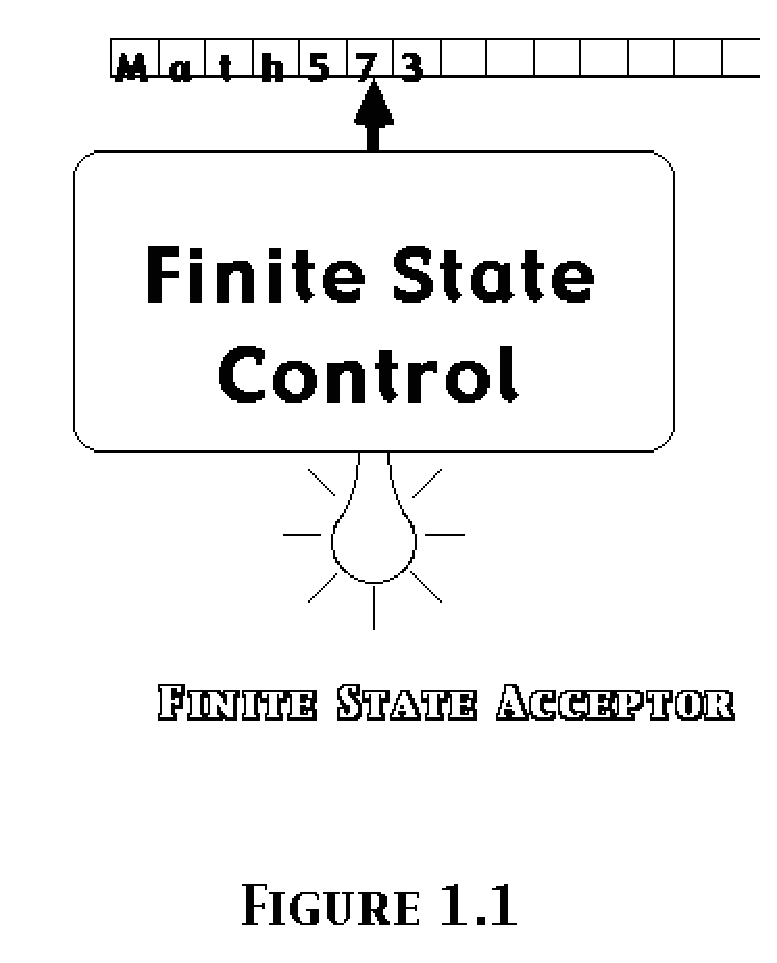
\epsfig{figure=Figures/fig-1-1.eps,height=2in}}
\centerline{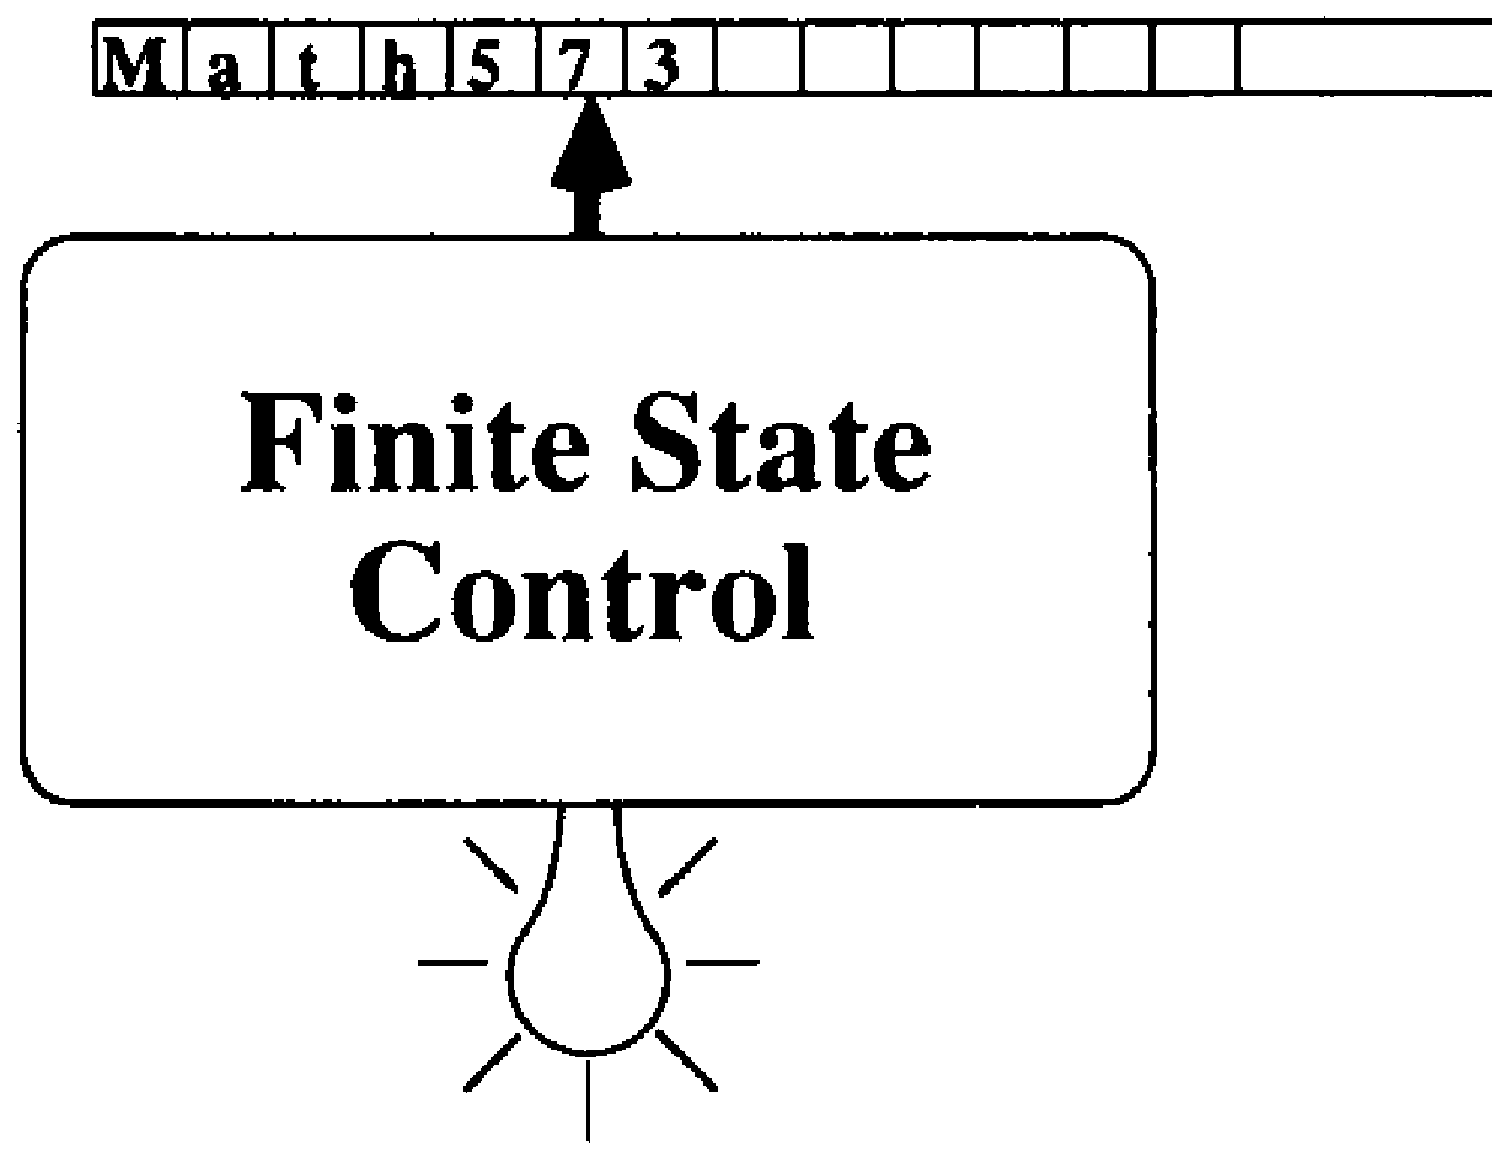
\epsfig{figure=ToFAfigures/fig1-1.eps,height=2in}}
\caption{A model of a finite-state acceptor (DFA)}\label{fig-1.1}
\end{figure}

Although finite automata are usually thought of as processing strings of letters
over some alphabet, the input can conceptually be elements from any finite set.
A useful example is the ``brain'' of a vending machine, which, say, dispenses
30\cent\ candy bars.

\subsection*{Example 1.5}

The input to the vending machine is the set of coins \{nickel, dime, quarter\},
represented by $\pmb{n}$, $\pmb{d}$, and $\pmb{q}$ in Figure \ref{fig-1.2}. The
machine may only ``remember'' a finite  number of things; in this case, it will
keep track of the amount of money that has been dropped into the machine. Thus,
the machine may be in the ``state'' of remembering that no money has yet been
deposited (denoted in this example by \<0\cent\>), or that a single nickel has
been inserted (the state labeled \<5\cent\>, or that either a dime or two
nickels have been deposited \<10\cent\>, and so on. Note that from state
\<0\cent\> there is an arrow labeled by the dime token $\pmb{d}$ pointing to the
state \<10\cent\>, indicating that, at a time when the machine ``believes'' that
no money has been deposited, the insertion of a dime causes the machine to
transfer to the state that remembers that ten cents has been deposited. From the
\<0\cent\> state, the arrows in the diagram show that if two nickels ($\pmb{n}$)
are input the machine moves through the \<5\cent\> state and likewise ends in
the state labeled \<10\cent\>.

The vending machine thus counts the amount of change dropped into the machine
(up to 50\cent). The machine begins in the state labeled \<0\cent\> and follows
the arrows to higher-numbered states as coins are inserted. For example,
depositing a nickel, a dime, and then a quarter would move the machine to the
states \<5\cent\>, \<15\cent\>, and then \<40\cent\>. The states labeled
30\cent\ and above are doubly encircled to indicate that enough money has been
deposited; if 30\cent\ or more has been deposited, then the machine ``accepts,''
indicating that a candy bar may be selected.\index{vending machine!DFA}

% Figure 1.2
\begin{figure}
%\centerline{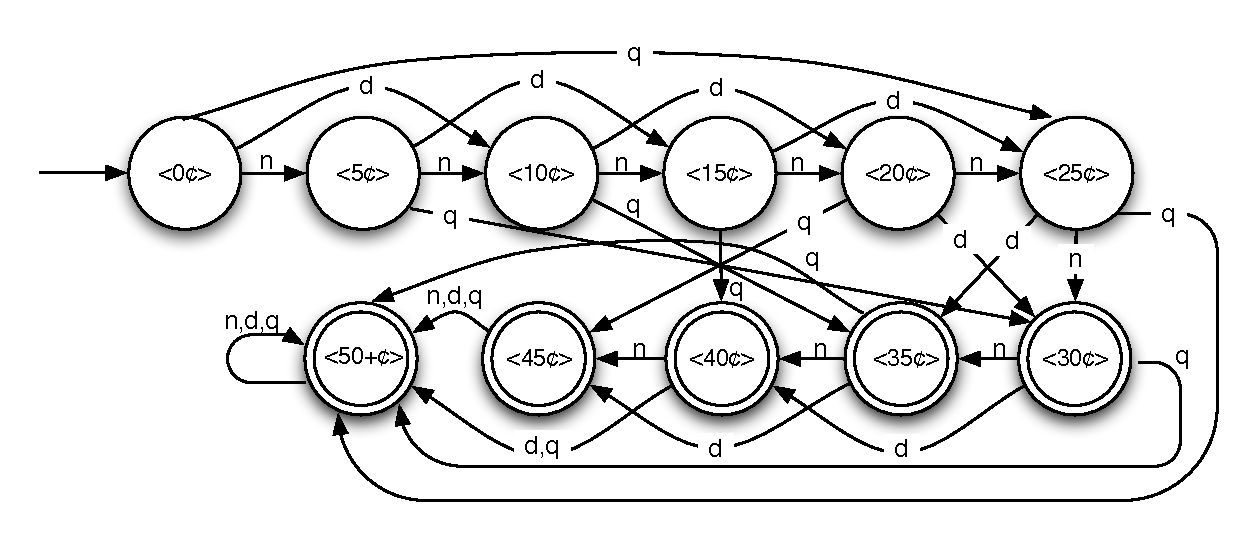
\epsfig{figure=Figures/fig-1-2.eps,width=\textwidth}}
\centerline{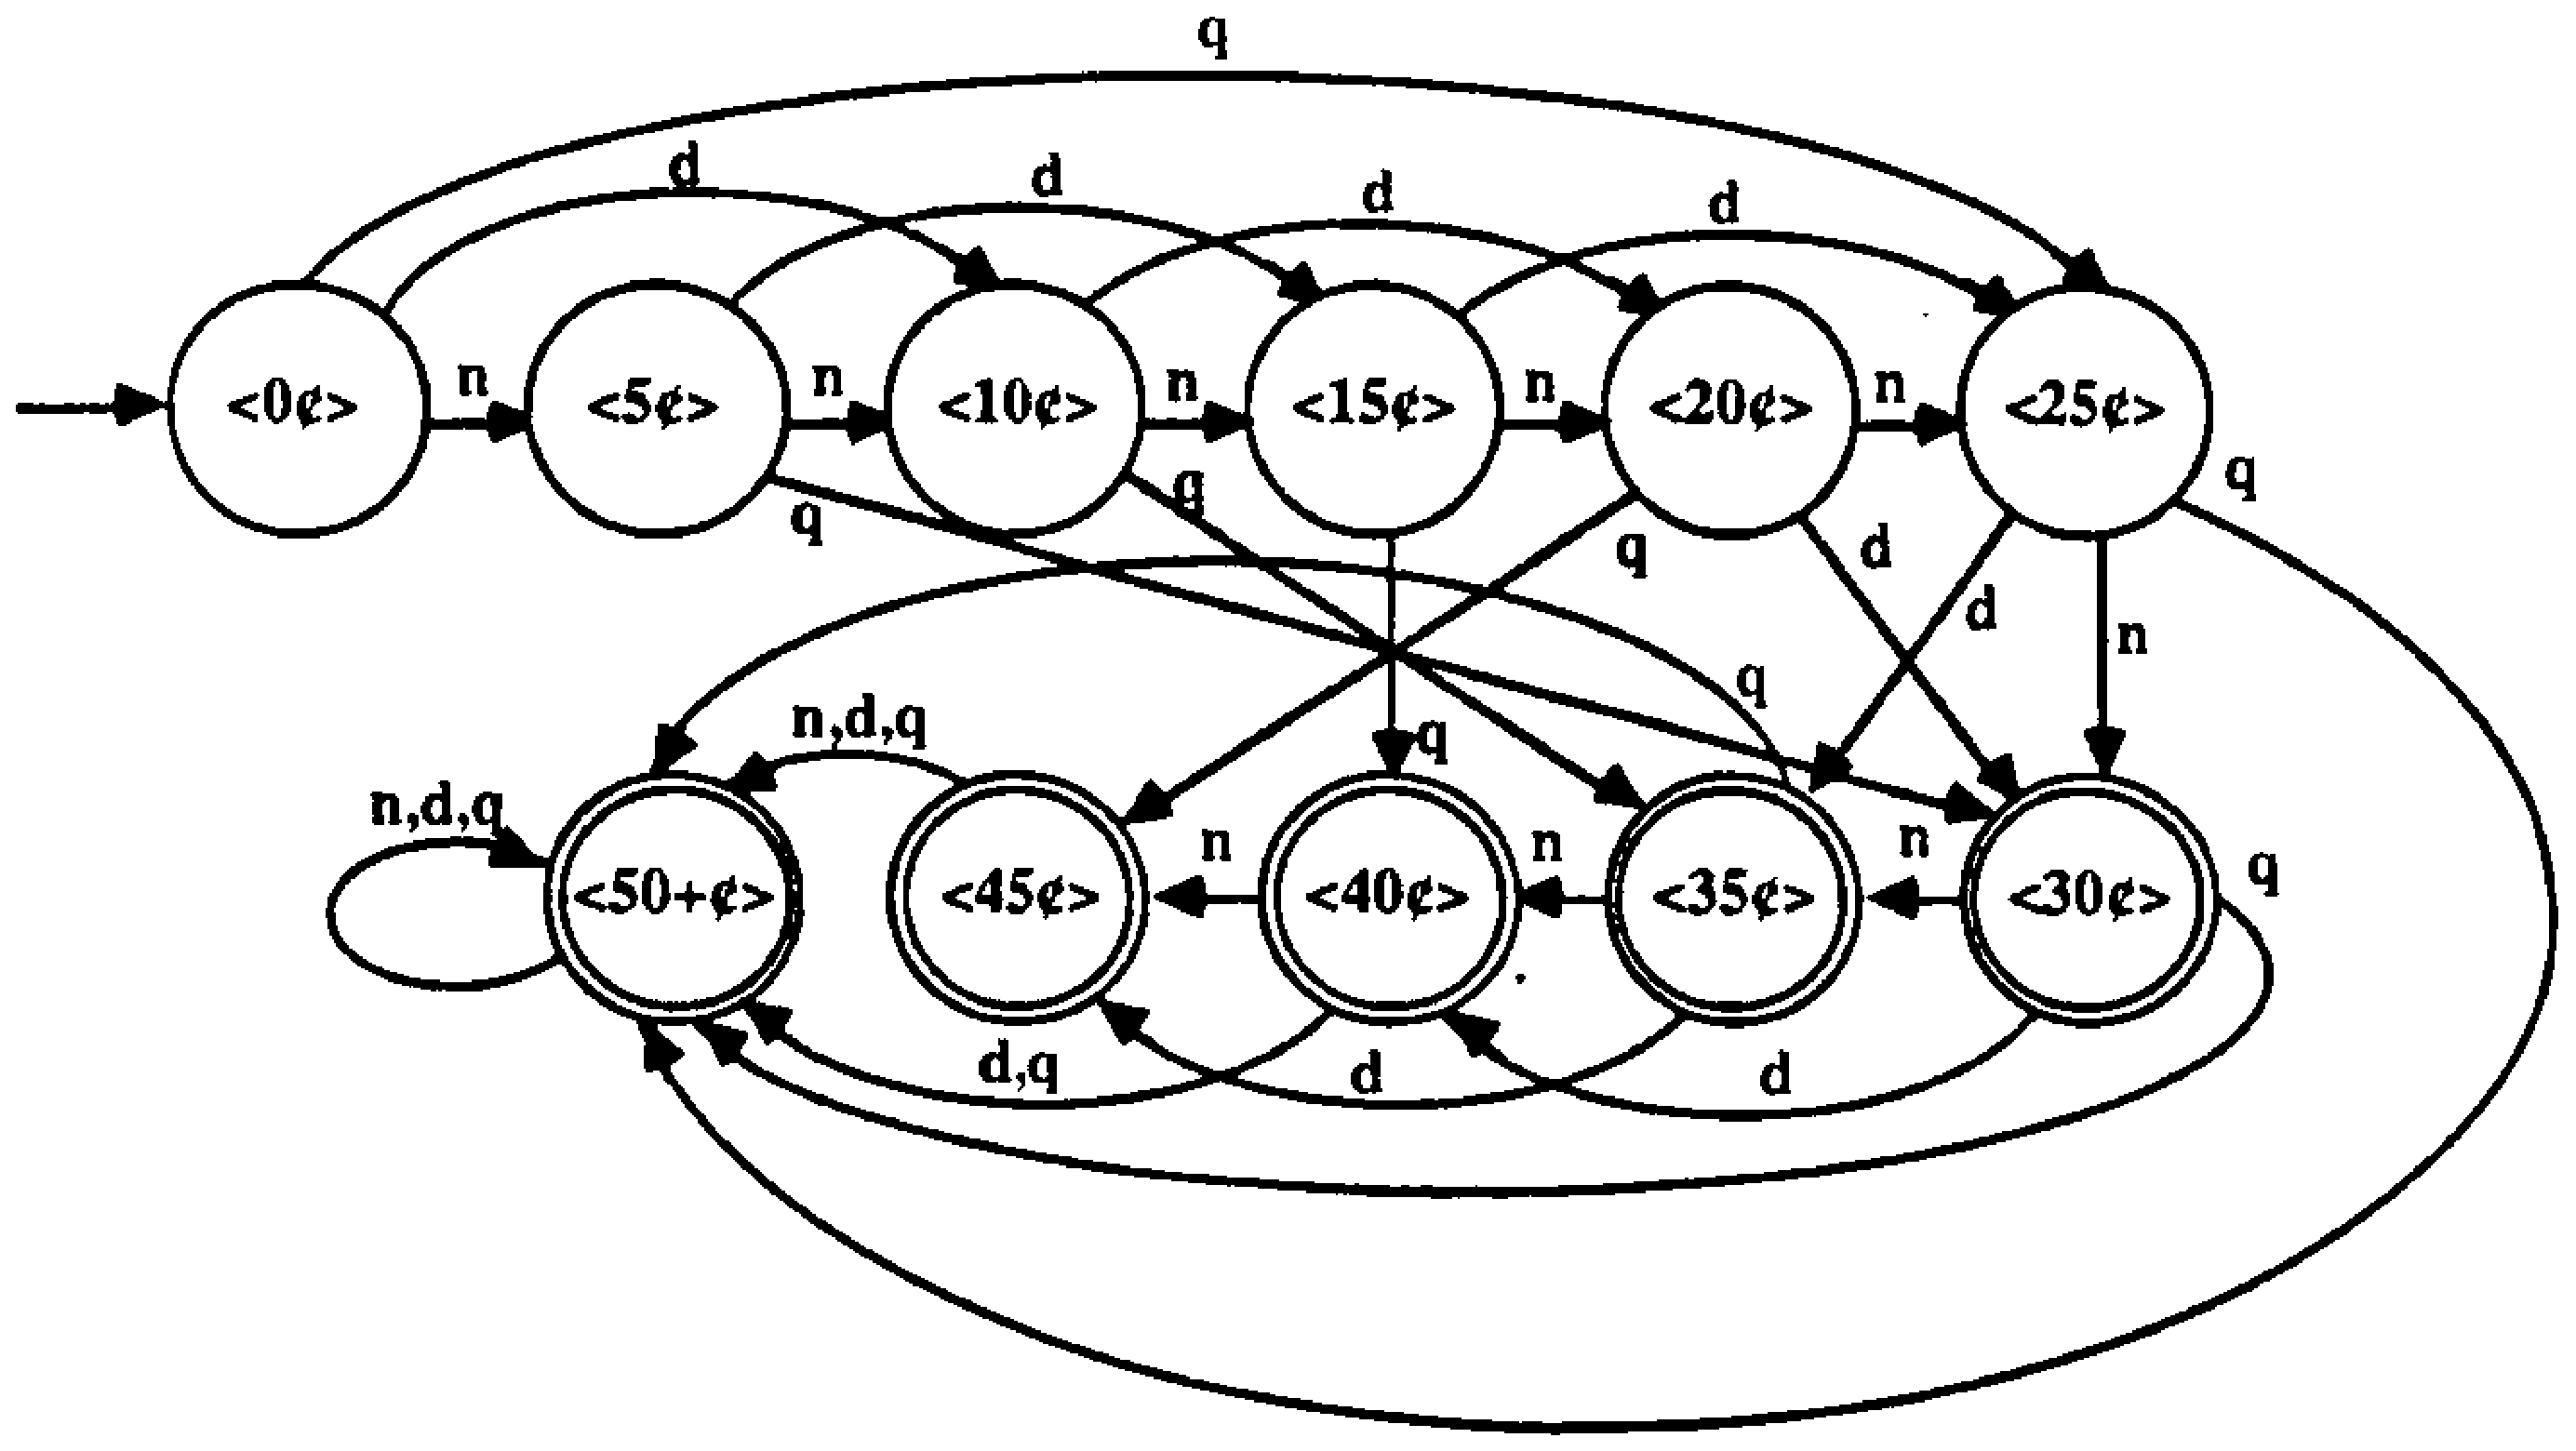
\epsfig{figure=ToFAfigures/fig1-2.eps,width=5in}}
\caption{An implementation of a vending machine}\label{fig-1.2}
\end{figure}

Finite automata are appropriate whenever there are a finite number of inputs and
only a finite number of situations must be distinguished by the machine. Other
applications include traffic signals and elevators (as discussed in Chapter
\ref{ch-7}). We now present a formal mathematical definition of a finite-state
machine.

% Definition 1.10
\begin{dfn}\label{dfn-1.10}\index{deterministic finite acceptor|see{DFA}}\index{final state!for DFA}\index{accepting state (DFA)}\index{alphabet!input}\index{D@ $\delta$ function|see{state transition function} }\index{state transition function!for DFA}

A \emph{deterministic finite automaton} or \emph{deterministic
finite acceptor} (\Index{DFA}) is a quintuple
\\$\langle\Sigma,S,s_0,\delta,F
\rangle$, where
\begin{enumerate}[i.]
\item $\Sigma$ is the \emph{input alphabet} (a finite nonempty set of symbols).
\item $S$ is a finite nonempty set of \emph{states}.
\item $s_0$ is the \emph{start} (or \emph{initial}) state,\index{start state}\index{initial state|see{start state}} an element of $S$.
\item $\delta$ is the \emph{state transition function};
	$\delta$: $S \times \Sigma \rightarrow S$.
\item $F$ is the set of \emph{final} (or \emph{accepting}) states, a (possibly
	empty) subset of $S$.
\end{enumerate}
\end{dfn}

The input alphabet, $\Sigma$, for any deterministic finite automaton A, is the
set of symbols that can appear on the input tape. Each successive symbol in a
word will cause a transition from the present state to another state in the
machine. As specified by the $\delta$ function, there is exactly one such state
transition for each combination of a symbol $a \in \Sigma$ and a state $s \in S$.
This is the origin of the word ``deterministic'' in the phrase ``deterministic
finite automaton.''\index{finite automaton!deterministic}

The various states represent the memory of the machine. Since the number of
states in the machine is finite, the number of distinguishable situations that
can be remembered by the machine is also finite. This limitation of the device's
ability to store its past history is the origin of the word ``finite'' in the
phrase ``deterministic finite automaton.'' At any given time during processing,
if the previous history of the machine is considered to be the reactions of the
DFA to the letters that have already been read, then the current state
represents all that is known about the history of the machine.

The start state of the machine is the state in which the machine always begins
processing a string. From this state, successive input symbols from $\Sigma$ are
used by the $\delta$ function to arrive at successive states in the machine.
Processing stops when the string of symbols is exhausted. The state in which the
machine is left can either be a final state, in which case the word is
\emph{accepted}, or it can be any one of the other states of $S$, in which case
the word is \emph{rejected}.\index{accept by final state}

To produce a formal description of the concepts defined above, it is necessary
to enumerate each part of the quintuple that comprises the DFA. $\Sigma$, $S$,
$s_0$, and $F$ are easily enumerated, but the function $\delta$ can often be
tedious to describe. One device used to display the mapping $\delta$ is the
\emph{state transition diagram}. Besides graphically displaying the transitions
of the $\delta$ function, the state transition diagram for a deterministic
finite automaton also illustrates the other four parts of the quintuple.

A finite automaton state transition diagram is a directed graph. The states of
the machine represent the vertices of the graph, while the mapping of the
$\delta$ function describes the edges. Final states are denoted by a doubly
encircled state, and the start state is identified by a straight incoming arrow.
Each domain element of the transition function corresponds to an edge in the
directed graph. We formally define a finite automaton state transition diagram
for $\langle\Sigma,S,s_0,\delta,F\rangle$ as a directed graph $G=\langle V,E
\rangle$, as follows:
\begin{enumerate}[i.]
\item $V=S$,
\item $E=\{\langle s,t,\pmb{a}\rangle | s,t\in S,\pmb{a}\in\Sigma\wedge\delta
	(s,\pmb{a})=t\}$,
\end{enumerate}
where $V$ is the set of vertices of the graph, and $E$ is the set of edges
connecting these vertices. Each element of $E$ is an ordered triple,
$\langle s,t,\pmb{a}\rangle$, such that $s$ is the origin vertex, $t$ is the
terminus, and $\pmb{a}$ is the letter from $\Sigma$ labeling the edge. Thus, for
any vertex there is exactly one edge leaving that vertex for each element of
$\Sigma$.

% Figure 1.3
\begin{figure}
%\centerline{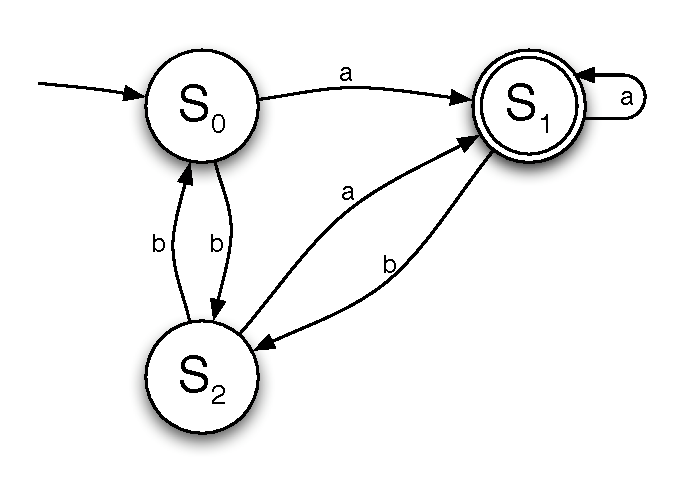
\epsfig{figure=Figures/fig-1-3.eps,width=\textwidth}}
\centerline{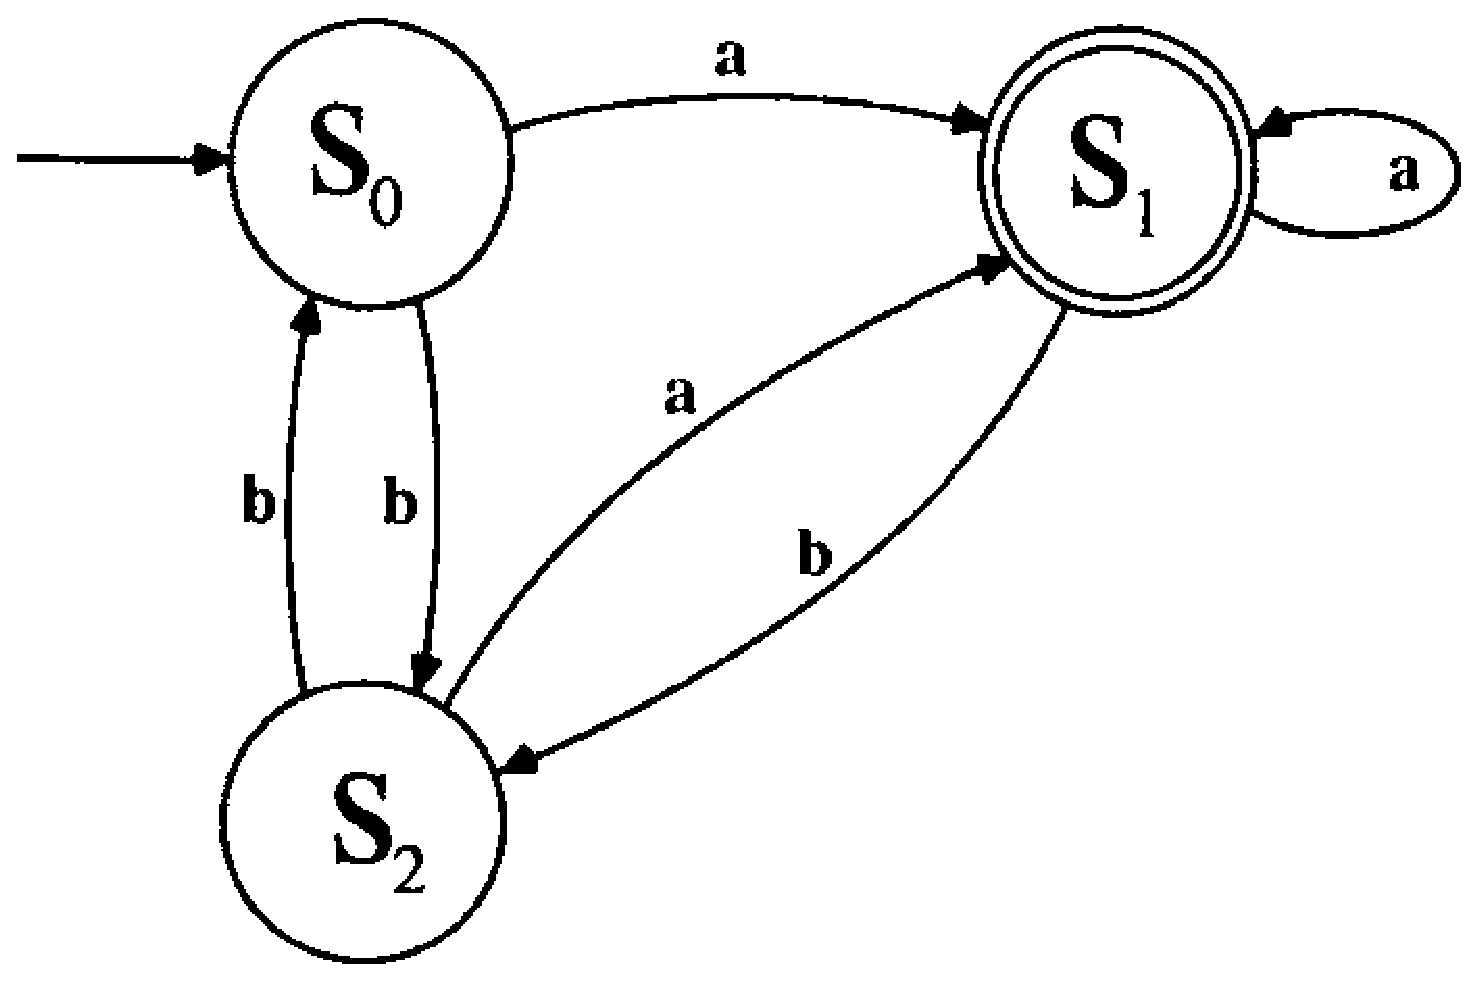
\epsfig{figure=ToFAfigures/fig1-3.eps,width=3in}}
\caption{The DFA described in Example 1.6}\label{fig-1.3}
\end{figure}

% Figure 1.4
\begin{center}
\begin{figure}
\begin{verbatim}
type
   Sigma = 'a'..'c';
   State = (s0,s1,s2);
var
   TransitionTable=array[State,Sigma] of State;

function Delta(S:State;A:Sigma):State;
begin
   Delta := TransitionTable [S, A]
end; {Delta}
\end{verbatim}
\caption{A Pascal implementation of a state transition function}\label{fig-1.4}
\end{figure}
\end{center}

\subsection*{Example 1.6}

In the DFA shown in Figure \ref{fig-1.3}, the set of edges $E$ of the graph $G$
is given by $E = \{\langle s_0,s_1,\pmb{a}\rangle,\langle s_0,s_2,\pmb{b}\rangle, \\
\langle s_1,s_1,\pmb{a}\rangle, \langle s_1,s_2,\pmb{b}\rangle, \langle s_2,s_1,
\pmb{a}\rangle,\langle s_2,s_0,\pmb{b}\rangle\}$. The figure also shows that
$s_0$ is the designated start state and that $s_1$ is the only final state. The
state transition function for a finite automaton is often represented in the
form of a \emph{state transition table}. A state transition table is a matrix
with the rows of the matrix labeled and indexed by the states of the machine,
and the columns of the matrix labeled and indexed by the elements of the input
alphabet; the entries in the table are the states to which the DFA will move.
Formally, let $T$ be a state transition table for some deterministic finite
automaton $A =\langle\Sigma,S,s_0,\delta,F\rangle$, and let $s \in S$ and
$\pmb{a}\in\Sigma$. Then the value of each matrix entry is given by the equation
\[ (\forall s\in S)(\forall\pmb{a}\in\Sigma)T_{s\pmb{a}}=\delta(s,\pmb{a}) \]
For the automaton in Example 1.6, the state transition table is
\begin{center}\begin{tabular}{c|cc}
$\delta$ & $\pmb{a}$ & $\pmb{b}$\\
\hline
$s_0$ & $s_1$ & $s_2$\\
$s_1$ & $s_1$ & $s_2$\\
$s_2$ & $s_1$ & $s_0$
\end{tabular}\end{center}
This table represents the following transitions:
\begin{align*}
&\delta(s_0,\pmb{a}) = s_1 &\delta(s_0,\pmb{b}) = s_2 \\
&\delta(s_1,\pmb{a}) = s_1 &\delta(s_1,\pmb{b}) = s_2 \\
&\delta(s_2,\pmb{a}) = s_1 &\delta(s_2,\pmb{b}) = s_0
\end{align*}

State transition tables are the most common method of representing the basic
structure of an automaton within a computer. When represented as an array in the
memory of the computer, access is very fast and the structure lends itself
easily to manipulation by the computer. Techniques such as depth-first search
are easily and efficiently implemented when the state transition diagram is
represented as a table. Figure \ref{fig-1.4} illustrates an implementation of
the $\delta$ function via transition tables in Pascal.

With $\delta$, we can describe the state in which we will find ourselves after
processing a single letter. We also want to be able to describe the state at
which we will arrive after processing an entire string. We will extend the
$\delta$ function to cover entire \emph{strings} rather than just single 
\emph{letters}; $\DBAR(s,x)$ will be the state we wind up at when
starting at $s$ and processing, in order, all the letters of the string $x$.
While this is a relatively easy concept to (vaguely) state in English, it is
somewhat awkward to formally define. To facilitate formal proofs concerning
DFAs, we use the following recursive definition.

% Definition 1.11
\begin{dfn}\label{dfn-1.11}\index{extended state transition function \DBAR\! for DFA}
\index{D@ $\overline \delta$|see{extended state transition function \DBAR}}
Given a DFA $A=\langle\Sigma,S,s_0,\delta,F\rangle$, the \emph{extended
state transition function for $A$}, denoted $\DBAR$, is a function $\DBAR$:
$S\times\Sigma^*\rightarrow S$ defined recursively as follows:
\\ \\
\begin{tabular}{r@{ }l@{$\qquad$}l@{ $=$ }l}
i. & $(\forall s\in S)(\forall\pmb{a}\in\Sigma)$ & $\DBAR(s,\pmb{a})$ &
	$\delta(s,\pmb{a})$ \\
ii. & $(\forall s\in S)$ & $\DBAR(s,\lambda)$ & $s$ \\
iii. & $(\forall s\in S)(\forall x\in\Sigma^*)(\forall\pmb{a}\in\Sigma)$ &
	$\DBAR(s,\pmb{a}x)$ & $\DBAR(\delta(s,\pmb{a}),x)$
\end{tabular}
\end{dfn}

The $\DBAR$ function extends the $\delta$ function from single
letters to words. Whereas the $\delta$ function maps pairs of states and
\emph{letters} to other states, the $\DBAR$ function maps pairs of
states and \emph{words} to other states. (i.) is the observation that $\delta$
and $\DBAR$ treat single letters the same; this fact is not really
essential to the definition of $\DBAR$, since it can be deduced from
(ii.) and (iii.) (see the exercises).

The $\DBAR$ function maps the current state $s$ and the first letter
$\pmb{a}_1$, of a word $w=\pmb{a}_1\ldots\pmb{a}_n$ via the $\delta$ function to
some other state $t$. It is then recursively applied with the new state $t$ and
the remainder of the word, that is, with $\pmb{a}_2\ldots\pmb{a}_n$. The
recursion stops when the remainder of the word is the empty word $\lambda$. See
Examples 1.7 and 1.11 for illustrations of computations using
this recursive definition.

Since the recursion of the $\DBAR$ function all takes place at the
end of the string, $\DBAR$ is called \emph{tail recursive}. \Index{Tail recursion}
is easily transformed into iteration by applying the $\delta$ to successive
letters of the input word and using the result of the previous application of
$\DBAR$ as an input to the current application.

Figure \ref{fig-1.5} gives an implementation of the $\DBAR$ function in
Pascal. Recursion has been replaced by iteration, and previous function results
are saved in an auxiliary variable T. The function Delta, the input alphabet
Sigma, and the state set State agree with the definitions given in Figure
\ref{fig-1.4}.

It stands to reason that if we start in state $s$ and word $y$ takes us to state
$r$, and if we start in state $r$ and word $x$ takes us to state $t$, then the
word $yx$ should take us from state $s$ all the way to $t$. That is, if
$\DBAR(s,y) = r$ and $\DBAR(r,x) = t$, then
$\DBAR(s,yx)$ should equal $t$, also. We can indeed prove this, as
shown with the following theorem.

% Theorem 1.1
\begin{thm}\label{thm-1.1}
Let $A =\langle\Sigma,S,s_0,\delta,F\rangle$ be a DFA. Then

\ \ \ \ \ \ \ \ \ \ \ \ \ \ \ \ \ \ \ \ 
$(\forall x \in \Sigma^*)(\forall y \in \Sigma^*)(\forall s \in S)
(\DBAR(s,yx) = \DBAR(\DBAR(s,y),x))$

\emph{Proof.} Define $P(n)$ by

\ \ \ \ \ \ \ \ \ \ \ \ \ \ \ \ \ \ \ \ 
$(\forall x \in \Sigma^*)(\forall y \in \Sigma^n)(\forall s \in S)
(\DBAR(s,yx) = \DBAR(\DBAR(s,y),x))$

\emph{Basis step}: $P(0)$: Let $y \in \Sigma^0 (\Rightarrow y = \lambda)$.
\begin{center}\begin{tabular}{l@{$\qquad$}l}
$\ \ \ \ \DBAR(\DBAR(s,y),x)$ & (since $y=\lambda$) \\
$=\DBAR(\DBAR(s,\lambda),x)$ & (by Definition \ref{dfn-1.11}ii)\\
$=\DBAR(s,x)$ & (since $x=\lambda\cdot x$) \\
$=\DBAR(s,\lambda x)$ & (since $y=\lambda$) \\
$=\DBAR(s,yx)$
\end{tabular}\end{center}

\emph{Inductive step}: Assume $P(m)$:
\[ (\forall x \in \Sigma^*)(\forall y \in \Sigma^m)(\forall s \in S)
	(\DBAR(s,yx) = \DBAR(\DBAR(s,y),x)), \]
For any $z \in \Sigma^{m+l},(\exists \pmb{a} \in \Sigma^1)(\exists y \in
\Sigma^m) \ni z = \pmb{a}y$. Then
\begin{center}\begin{tabular}{r@{ }l@{$\qquad$}l}
& $\DBAR(s,zx)$ & (by definition of $z$) \\
$=$ & $\DBAR(s,\pmb{a}yx)$ & (by Definition \ref{dfn-1.11}iii) \\ 
$=$ & $\DBAR(\delta(s,\pmb{a}),yx)$ & (since $(\exists t\in S)\ni\delta(s,
	\pmb{a})=t)$ \\
$=$ & $\DBAR(t,yx)$ & (by the induction assumption) \\
$=$ & $\DBAR(\DBAR(t,y),x)$ & (by definition of $t$) \\ 
$=$ & $\DBAR(\DBAR(\delta(s,\pmb{a}),y),x)$ & (by Definition \ref{dfn-1.11}iii) \\
$=$ & $\DBAR(\DBAR(s,\pmb{a}y),x)$ & (by definition of $z$) \\
$=$ & $\DBAR(\DBAR(s,z),x)$ \\
\end{tabular}\end{center}
Therefore, $P(m)\Rightarrow P(m+1)$, and since this implication holds for any
nonnegative integer $m$, by the principle of mathematical induction we can say
that $P(n)$ is true for all $n \in \NN$. Since the statement therefore holds for
any string $y$ of any length, the assertion is indeed true for all $y$ in
$\Sigma^*$. This completes the proof of the theorem.
\end{thm}

Note that the statement of Theorem \ref{thm-1.1} is very similar to the rule iii
of the recursive definition of the extended state transition function
(Definition \ref{dfn-1.11}) with the \emph{string} $y$ replacing the single
\emph{letter} $\pmb{a}$. We will see a remarkable number of situations like this,
where a recursive rule defined for a single symbol extends in a natural manner
to a similar rule for arbitrary strings.

As alluded to earlier, the state in which a string terminates is significant; in
particular, it is important to determine whether the terminal state for a string
happens to be one of the states that was designated to be a \emph{final} state.

% Definition 1.12
\begin{dfn}\label{dfn-1.12}\index{accept by final state}
Given a DFA $A = \langle\Sigma,S,s_0,\delta,F\rangle$, A \emph{accepts} a word
$w \in \Sigma^*$ iff \ \  $\DBAR(s_0,w) \in F$.
\end{dfn}

% Figure 1.5
\begin{figure}
\begin{verbatim}
const
MaxWordLength = 255; {an arbitrary constraint} 
type 
   Word = record 
      Length :0..MaxWordLength; 
      Letters:packed array [0..MaxWordLength] of Sigma 
   end; {Word} 
function DeltaBar(S:State; W:Word) : State; 
{uses the function Delta defined previously} 
var 
   T:State; 
   I:0..MaxWordLength; 
begin 
   T := S; 
   if W.Length>0 
      then 
         for I := 1 to W.Length do 
            T := Delta(T, W.Letters[I]); 
   DeltaBar := T
end; {DeltaBar}
\end{verbatim}
\caption{A Pascal implementation of the extended state transition function}\label{fig-1.5}
\end{figure}

We say a word $w$ is accepted by a machine $A = \langle\Sigma,S,s_0,\delta,F
\rangle$ \emph{iff} the extended state transition function $\delta$ associated
with $A$ maps to a final state from $s_0$ when processing the word $w$. This
means that the path from the start state ultimately leads to a final state when
the word $w$ is presented to the machine. We will occasionally say that $A$
\emph{recognizes} $w$; a DFA is sometimes referred to as a
\emph{\Index{recognizer}}.

% Definition 1.13
\begin{dfn}\label{dfn-1.13}
Given a DFA $A = \langle\Sigma,S,s_0,\delta,F\rangle$, $A$ \emph{rejects} a word $w \in
\Sigma^*$ iff \ \  $\DBAR(s_0,w) \notin F$.
\end{dfn}

In other words, a word $w$ is rejected by a machine
$A = \langle\Sigma,S,s_0,\delta,F\rangle$ \emph{iff} the $\DBAR$ function associated
with $A$ maps to a nonfinal state from $s_0$ when processing the word $w$.

\subsection*{Example 1.7}

Let
\begin{center}\begin{tabular}{r@{ $=$ }l}
$A$ & $\langle\Sigma,S,s_0,\delta,F\rangle$
\end{tabular}\end{center}
where
\begin{center}\begin{tabular}{r@{ $=$ }l}
$\Sigma$ & $\{\pmb{0},\pmb{1}\}$ \\
$S$ & $\{q_0,q_1\}$ \\
$s_0$ & $q_0$ \\
$F$ & $\{q_1\}$
\end{tabular}\end{center}
and $\delta$ is given by the transition table
\begin{center}\begin{tabular}{c|cc}
$\delta$ & $\pmb{0}$ & $\pmb{1}$ \\
\hline
$q_0$ & $q_0$ & $q_1$ \\
$q_1$ & $q_1$ & $q_0$
\end{tabular}\end{center}
The structure of this automaton is shown in Figure \ref{fig-1.6}.

To see how some of the above definitions apply, let $x = \pmb{0100}$:
\begin{align*}
\DBAR(q_0,x) &= \DBAR(q_0, \pmb{0100}) \\
&= \DBAR(\delta(q_0,\pmb{0}), \pmb{100}) \\
&= \DBAR(q_0, \pmb{100}) \\
&= \DBAR(\delta(q_0, \pmb{1}),\pmb{00}) \\
&= \DBAR(q_1, \pmb{00}) \\
&= \DBAR(\delta(q_1, \pmb{0}), \pmb{0}) \\
&= \DBAR(q_1, \pmb{0}) \\
&= \delta(q_1, \pmb{0}) \\
&= q_1
\end{align*}
Thus, $\DBAR(q_0,x) = q_1 \in F$, which means that $x$ is 
\emph{accepted} by $A$; $A$ \emph{recognizes} $x$.

Now let $y = \pmb{1100}$:
\begin{align*}
\DBAR(q_0,y) &= \DBAR(q_0, \pmb{1100}) \\
&= \DBAR(\delta(q_0,\pmb{1}), \pmb{100}) \\
&= \DBAR(q_1, \pmb{100}) \\
&= \DBAR(\delta(q_1, \pmb{1}),\pmb{00}) \\
&= \DBAR(q_0, \pmb{00}) \\
&= \DBAR(\delta(q_0, \pmb{0}), \pmb{0}) \\
&= \DBAR(q_0, \pmb{0}) \\
&= \delta(q_0, \pmb{0}) \\
&= q_0
\end{align*}
Therefore, $\DBAR(q_0,y) = q_0 \notin F$, which means that $y$ is
\emph{not accepted} by $A$.

Following the Pascal conventions defined in the previous programming fragments,
the function \emph{Accept} defined in Figure \ref{fig-1.7} tests for acceptance
of a string by consulting a FinalState set and using DeltaBar to refer to the
TransitionTable.

% Figure 1.6
\begin{figure}
%\centerline{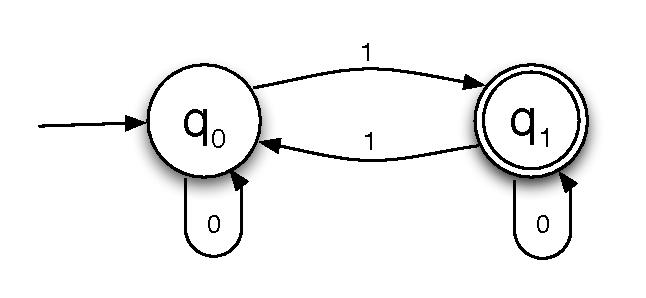
\epsfig{figure=Figures/fig-1-6.eps,width=\textwidth}}
\centerline{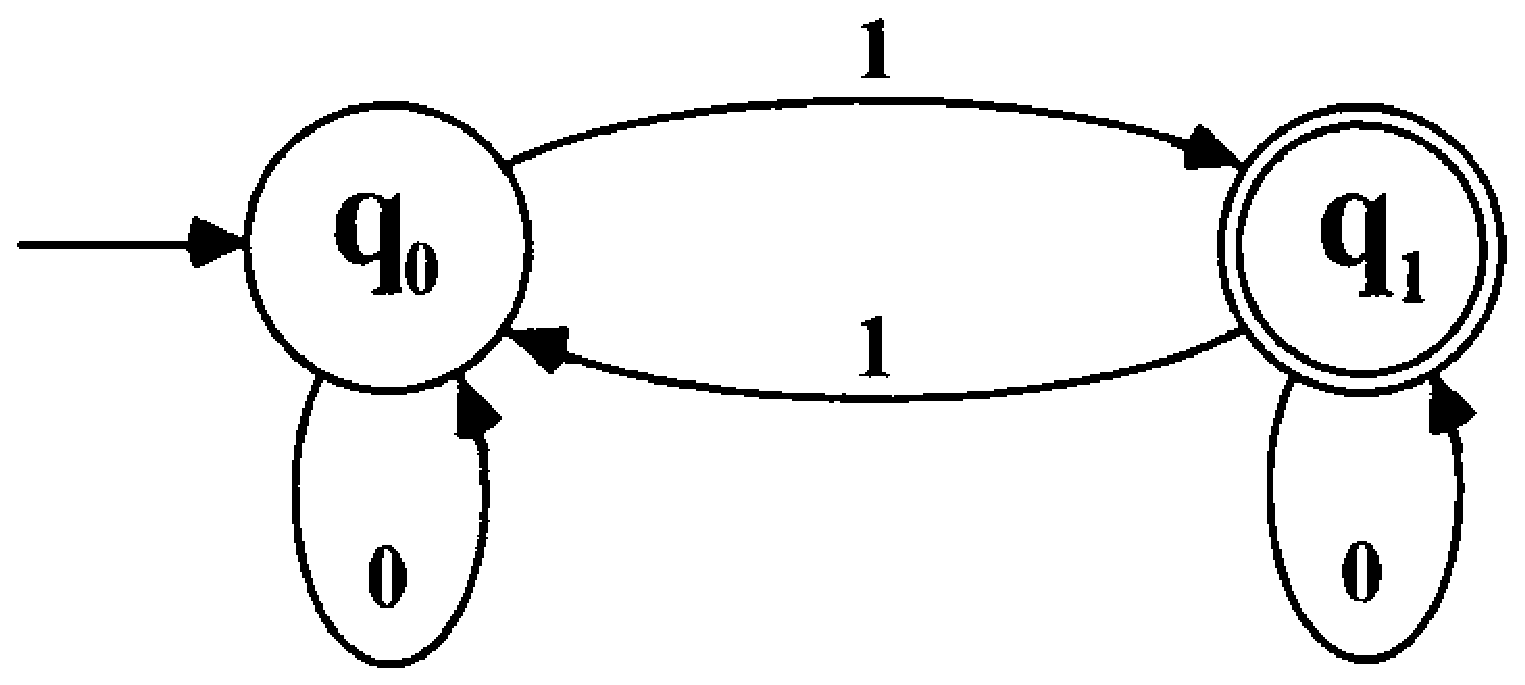
\epsfig{figure=ToFAfigures/fig1-6.eps,width=3in}}
\caption{The DFA discussed in Example 1.7}\label{fig-1.6}
\end{figure}

The functions \texttt{Delta}, \texttt{DeltaBar}, and \texttt{Accept} can be
combined to form a Pascal program that models a DFA. The sample fragments given
in Figures \ref{fig-1.4}, \ref{fig-1.5}, and \ref{fig-1.7} rightly pass the
candidate string as a parameter. A full program would be complicated by several
constraints, including the awkward way in which strings must be handled in
Pascal. To highlight the correspondence between the code modules and the
automata definitions, the program given in Figure \ref{fig-1.8} handles input at
the character level rather than at the word level. The definitions in the
procedure \texttt{Initialize} reflect the structure of the DFA shown in Figure
\ref{fig-1.9}. Invoking this program will produce a response to a single input
word. For example, a typical exchange would be
\begin{align*}
\pmb{cba} & \\
\text{Rejected} & \\
\intertext{Running this program again might produce}
\pmb{cccc} & \\
\text{Accepted} & \\
\end{align*}
This behavior is essentially the same as that of the C program shown
in Figure \ref{fig-1.10}. The succinct coding clearly shows the relationship
between the components of the quintuple for the DFA and the corresponding code.

% Definition 1.14
\begin{dfn}\label{dfn-1.14}
Given an alphabet $\Sigma$, $L$ is a \emph{\Index{language}} over the alphabet
$\Sigma$ iff $L \subseteq \Sigma^*$.
\end{dfn}

A language is a collection of words over some alphabet. If the alphabet is
denoted by $\Sigma$, then a language $L$ over $\Sigma$ is a subset of
$\Sigma^*$. Since $L \subseteq \Sigma^*$, $L$ may be finite or infinite.
Clearly, the words used in the English language are a subset of words over the
Roman alphabet and this collection is therefore a language according to our
definition. Note that a language $L$, in this context, is simply a list of
words; neither syntax nor semantics are involved in the specification of $L$.
Thus, a language as defined by Definition \ref{dfn-1.14} has little of the
structure or relationships one would normally expect of either a natural
language (like English) or a programming language (like Pascal).

% Figure 1.7
\begin{figure}
\begin{verbatim}
function Accept(W:Word):Boolean;
{returns TRUE iff W is accepted by the DFA}
begin
   Accept := DeltaBar(s0, W) in FinalState
end; {Accept}
\end{verbatim}
\caption{A Pascal implementation of a test for acceptance}\label{fig-1.7}
\end{figure}

% Figure 1.8
\begin{figure}
\begin{verbatim}
program DFA(input, output);
{This program tests whether input strings are accepted by the     }
{automaton displayed in Figure 1.9. The program expects input from}
{the keyboard, delimited by a carriage return. No error checking  }
{is done; letters outside ['a' .. 'c'] cause a range error.       }
type
    Sigma = 'a'..'c';
    State = (s0, s1, s2);
var
    TransitionTable : array [State, Sigma] of State;
    FinalState	     : set of State;
function Delta(s : State; c : Sigma) : State;
begin
    Delta := TransitionTable[s,c]
end; { Delta }
function DeltaBar(s : State) : State;
var
    t : State;
begin
    t := s;
    { Step through the keyboard input one letter at a time. }
    while not eoln(input) do
        begin
	    t := Delta(t, input^);
	    get(input)
	end;
    DeltaBar := t
end; { DeltaBar }
function Accept : boolean;
begin
    Accept := DeltaBar(s0) in FinalState
end; { Accept }
procedure Initialize;
begin
    FinalState := [s2];
    { Set up the state transition table. }
    TransitionTable [s0,'a'] := s1; TransitionTable [s0,'b'] := s0;
    TransitionTable [s0,'c'] := s2; TransitionTable [s1,'a'] := s2;
    TransitionTable [s1,'b'] := s0; TransitionTable [s1,'c'] := s0;
    TransitionTable [s2,'a'] := s0; TransitionTable [s2,'b'] := s0;
    TransitionTable [s2,'c'] := s1;
end; { Initialize }
begin { DFA }
    Initialize;
    if Accept then
        writeln(output, 'Accepted')
    else
        writeln(output, 'Rejected')
end. { DFA }
\end{verbatim}
\caption{A Pascal program that emulates the DFA shown in Figure \ref{fig-1.9}}\label{fig-1.8}
\end{figure}

% Figure 1.9
\begin{figure}\index{finite automaton!Pascal implementation}
%\centerline{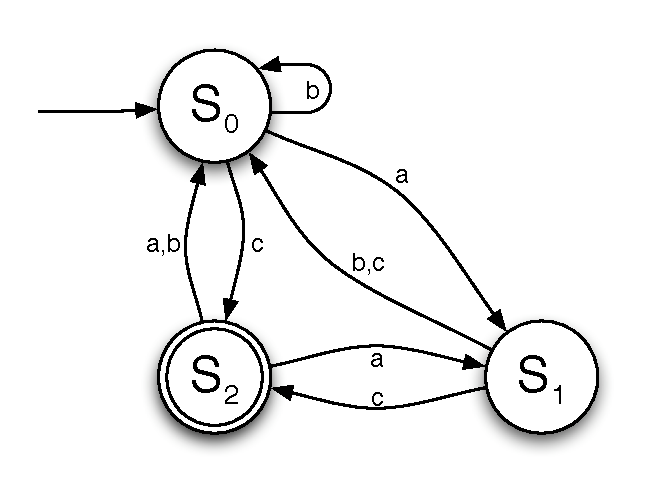
\epsfig{figure=Figures/fig-1-9.eps,width=\textwidth}}
\centerline{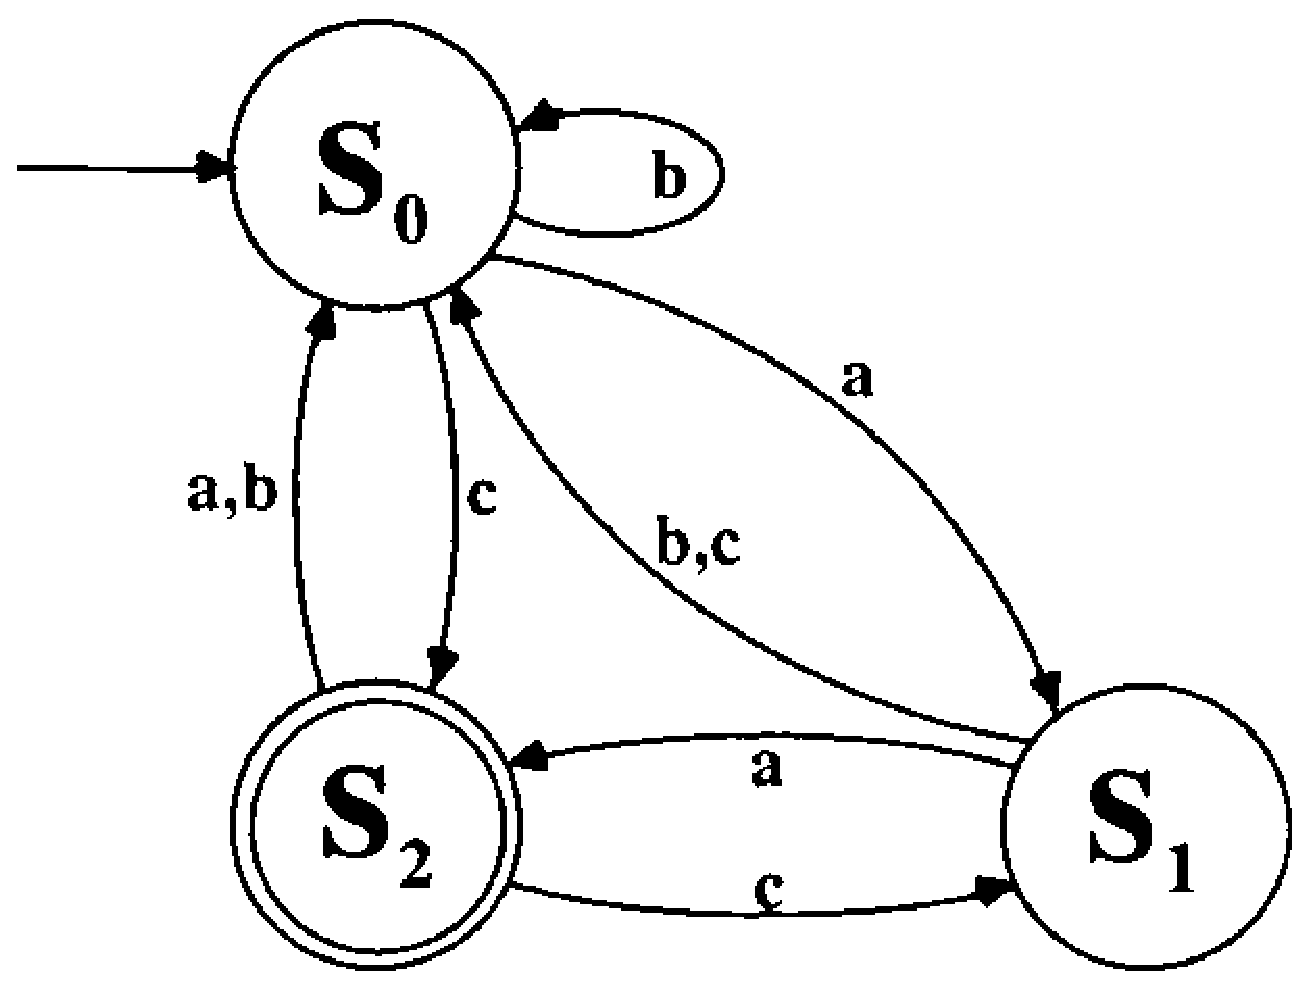
\epsfig{figure=ToFAfigures/fig1-9.eps,width=3in}}
\caption{The DFA emulated by the programs in Figures \ref{fig-1.8} and
\ref{fig-1.10}}\label{fig-1.9}
\end{figure}

\subsection*{Example 1.8}

Some other examples of valid languages are
\begin{enumerate}[i.]
\item $\emptyset$
\item $\{w \in\{\pmb{0},\pmb{1}\}^*\ | \ \ \ |w| > 5\}$
\item $\{\lambda\}$
\item \{$\lambda$, {\bf bilbo}, {\bf frodo}, {\bf samwise}\}
\item $\{x \in \{\pmb{a},\pmb{b}\}^*\ | \ \ \ |x|_{\pmb{a}} = |x|_{\pmb{b}}\}$
\end{enumerate}

% Figure 1.10
\begin{figure}
\begin{verbatim}
# include       <stdio.h>
# define        to_int(c)       ((int) c-(int) 'a')
# define        FINAL_STATE     s_2

enum state { s_0, s_1, s_2 };
/*
** This table implements the state transition function and is indexed by
** the current state and the current input letter.
*/
enum state transition_table[3][3]={ { s_1, s_0, s_2 },
                                    { s_2, s_0, s_0 },
                                    { s_0, s_0, s_1 }};
enum state delta(enum state s, char c) {
        return transition_table[(int) s][to_int(c)];
}
enum state delta_bar(enum state s) {
        enum state t;
        char       c;
	
        t=s;
/*
** Step through the input one letter at a time.
*/
        while ((char) (c = getchar()) != '\n')
              t=delta(t, c);
        return t;
}
main() {
        if (delta_bar(s_0) == FINAL_STATE)
                printf("Accepted\n");
        else
                printf("Rejected\n");
        exit(0);
}
\end{verbatim}
\caption{A C program that emulates the DFA shown in Figure \ref{fig-1.9}}\label{fig-1.10}\index{finite automaton!C implementation}
\end{figure}

The empty language, denoted by $\emptyset$ or $\{\ \ \}$, is different from
$\{\lambda\}$, the language consisting of only the empty word $\lambda$. Whereas
the empty language consists of zero words, the language consisting of $\lambda$
contains one word (which contains zero letters). The distinction is analogous to
an example involving sets of numbers: the set $\{0\}$, containing only the
integer $0$, is still a larger set than the empty set.

Every DFA differentiates between words that do not reach final states and 
words that do. In this sense, each automaton defines a language.

% Definition 1.15
\begin{dfn}\label{dfn-1.15}
Given a DFA $A = \langle\Sigma,S,s_0,\delta,F\rangle$, the \emph{language accepted by}
$A$, denoted $L(A)$, is defined to be 
$$L(A) = \{w \in \Sigma^*\ | \ \DBAR(s_0, w) \in F\}$$
\end{dfn}

$L(A)$, the language accepted by a finite automaton $A$, is the set of all words
$w$ from $\Sigma^*$ for which $\DBAR(s_0, w) \in F$. In order for a
word $w$ to be contained in $L(B)$, the path through the finite automaton B, as
determined by the letters in $w$, must lead from the start state to one of the
final states.

For deterministic finite automata, the path for a given word $w$ is unique:
there is only one path since, at any given state in the automaton, there is
exactly one transition for each $a \in \Sigma$. This is not necessarily the case
for another variety of finite automaton, the \emph{nondeterministic} finite
automaton, as will be seen in Chapter \ref{ch-4}.

% Definition 1.16
\begin{dfn}\label{dfn-1.16}\index{finite automaton definable}
Given an alphabet $\Sigma$, a language $L \subseteq \Sigma^*$ is 
\emph{finite automaton definable} (FAD) iff there exists some DFA
$B =\ \langle\Sigma,S,s_0,\delta,F\rangle$, such that $L = L(B)$.
\end{dfn}

The set of all words over $\{\pmb{0,1}\}$ that contain an odd number of
\pmb{1}s is finite
automaton definable, as evidenced by the automaton in Example 1.7,
which accepts exactly this set of words.

\section{Examples of Finite Automata}\label{sec-1.3}

This section illustrates the definitions of the quintuples and the state
transition diagrams for some nontrivial automata. The following example and
Example 1.11 deal with the recognition of tokens, an important issue in
the construction of compilers.

\subsection*{Example 1.9}\index{ASCII alphabet}

The set of FORTRAN identifiers is a finite automaton definable language. This
statement can be proved by verifying that the following machine accepts the set
of all valid FORTRAN 66 identifiers. These identifiers, which represent
variable, subroutine, and array names, can contain from 1 to 6 (nonblank)
characters, must begin with an alphabetic character, can be followed by up to 5
letters or digits, and may have embedded blanks. In this example, we have
ignored the difference between capital and lowercase letters,
and $\diamond$ represents a blank.\index{blank symbol}

\begin{align*}
\Sigma &=\text{ ASCII} \\
\Gamma &=\text{ ASCII} - \{\pmb{a},\pmb{b},\pmb{c,}\ldots\pmb{x},\pmb{y},\pmb{z},
	\pmb{0},\pmb{1},\pmb{2},\pmb{3},\pmb{4},\pmb{5},\pmb{6},\pmb{7},\pmb{8},
	\pmb{9},\diamond\} \\
S &= \{s_0,s_1,s_2,s_3,s_4,s_5,s_6,s_7\} \\
s_0 &= s_0
\end{align*}

\begin{center}
\begin{tabular}{c|ccccccccc}
$\delta$ & $\pmb{a}$ & $\pmb{b}$ & $\pmb{c}\ldots\pmb{y}$ & $\pmb{z}$ & $\pmb{0}$
	& $\pmb{1}\ldots\pmb{8}$ & $\pmb{9}$ & $\diamond$ & $\Gamma$ \\
\hline
$s_0$ & $s_1$ & $s_1$ & $s_1\ldots s_1$ & $s_1$ & $s_7$ & $s_7\ldots s_7$
	& $s_7$ & $s_0$ & $s_7$ \\
$s_1$ & $s_2$ & $s_2$ & $s_2\ldots s_2$ & $s_2$ & $s_2$ & $s_2\ldots s_2$
	& $s_2$ & $s_1$ & $s_7$ \\ 
$s_2$ & $s_3$ & $s_3$ & $s_3\ldots s_3$ & $s_3$ & $s_3$ & $s_3\ldots s_3$
	& $s_3$ & $s_2$ & $s_7$ \\
$s_3$ & $s_4$ & $s_4$ & $s_4\ldots s_4$ & $s_4$ & $s_4$ & $s_4\ldots s_4$
	& $s_4$ & $s_3$ & $s_7$ \\
$s_4$ & $s_5$ & $s_5$ & $s_5\ldots s_5$ & $s_5$ & $s_5$ & $s_5\ldots s_5$
	& $s_5$ & $s_4$ & $s_7$ \\
$s_5$ & $s_6$ & $s_6$ & $s_6\ldots s_6$ & $s_6$ & $s_6$ & $s_6\ldots s_6$
	& $s_6$ & $s_5$ & $s_7$ \\
$s_6$ & $s_7$ & $s_7$ & $s_7\ldots s_7$ & $s_7$ & $s_7$ & $s_7\ldots s_7$
	& $s_7$ & $s_6$ & $s_7$ \\
$s_7$ & $s_7$ & $s_7$ & $s_7\ldots s_7$ & $s_7$ & $s_7$ & $s_7\ldots s_7$
	& $s_7$ & $s_7$ & $s_7$
\end{tabular}
$$F = \{s_1,s_2,s_3,s_4,s_5,s_6\}$$
\end{center}

The entries under the column labeled $\Gamma$ show the transitions taken for
each member of the set $\Gamma$. The state transition diagram of the machine
corresponding to this quintuple is displayed in Figure \ref{fig-1.11}. Note
that, while each of the 26 letters transition from $s_0$ to $s_1$, a single
arrow labeled \pmb{a}-\pmb{z} is sufficient to denote all these transitions. Similarly, the
transition labeled $\Sigma$ from $s_7$ indicates that every element of the
alphabet follows the same path.

% Figure 1.11
\begin{figure}
\centerline{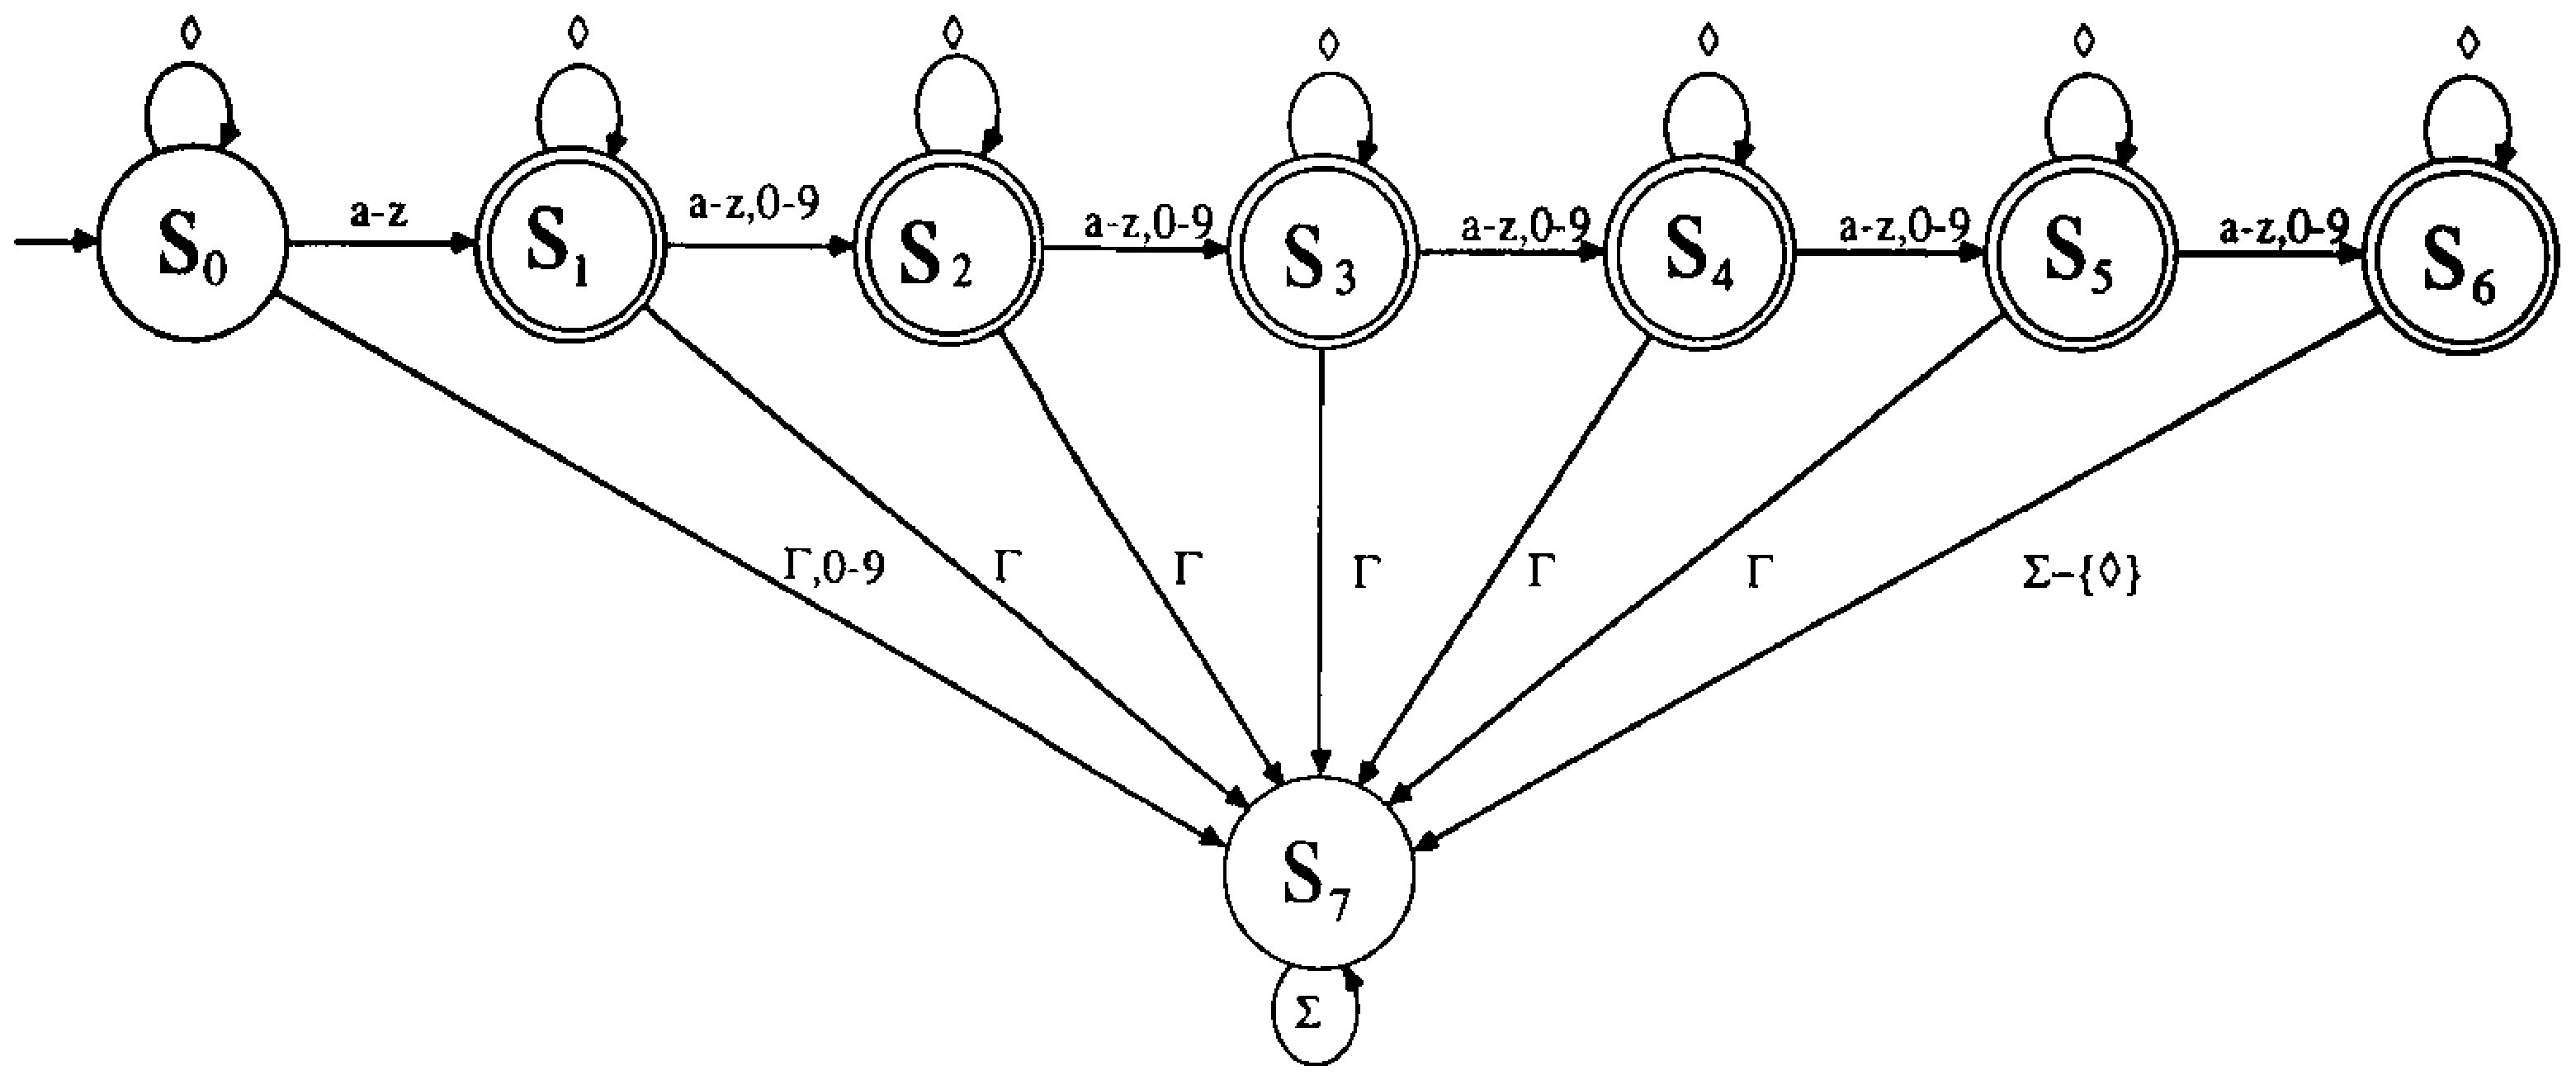
\epsfig{figure=ToFAfigures/fig1-11.eps,width=6.5in}}
\caption{A DFA that recognizes valid FORTRAN identifiers}\label{fig-1.11}
\end{figure}

% Figure 1.12
\begin{figure}
\centerline{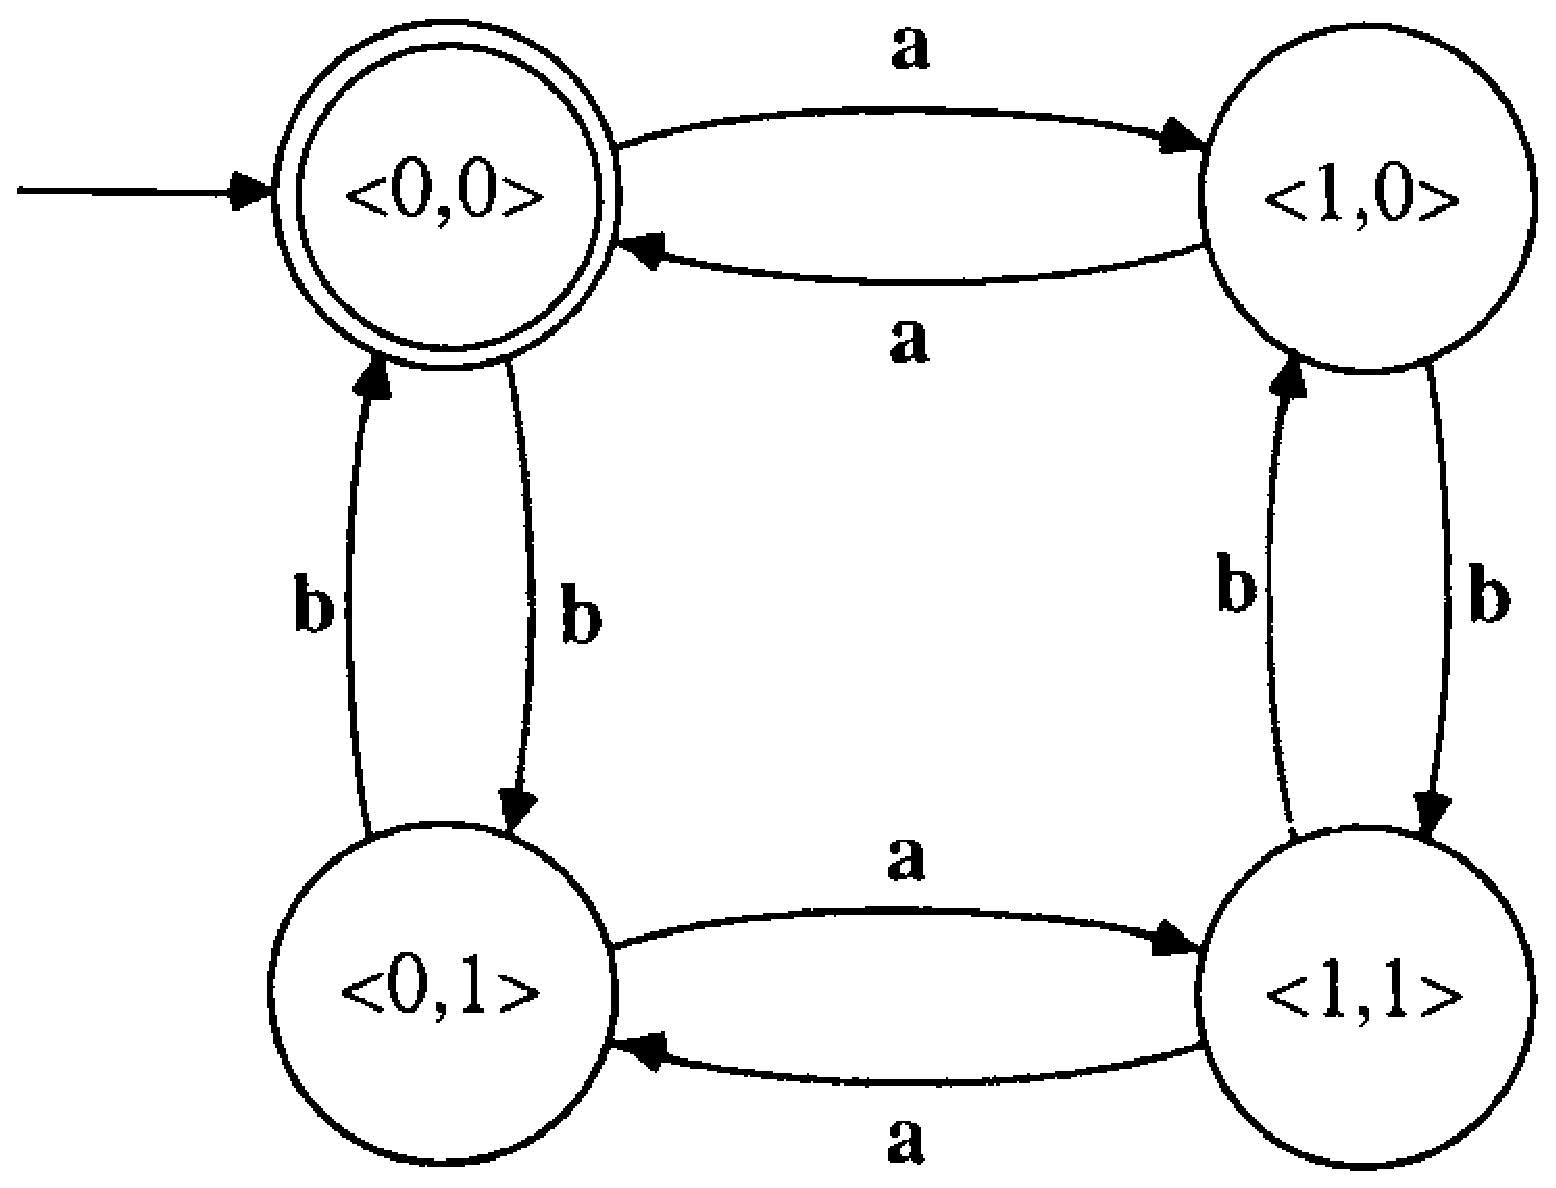
\epsfig{figure=ToFAfigures/fig1-12.eps,width=2.7in}}
\caption{The DFA $M$ discussed in Example 1.10}\label{fig-1.12}
\end{figure}

\subsection*{Example 1.10}

The DFA $M$ shown in Figure \ref{fig-1.12} accepts only those strings that have an even
number of $\pmb{b}$s and an even number of $\pmb{a}$s. Thus
$$L(M) = \{x \in \{\pmb{a},\pmb{b}\}^* \ | \ \ \ |x|_{\pmb{a}} \equiv 0 \bmod 2 \wedge
	|x|_{\pmb{b}} \equiv 0\bmod 2\}$$
The corresponding quintuple for $M = \langle\Sigma,S,s_0,\delta,F\rangle$ has the
following components:
\begin{align*}
\Sigma &= \{\pmb{a},\pmb{b}\} \\
S &= \{\langle 0,0\rangle,\langle 0,1\rangle,\langle 1,0\rangle,\langle 1,1\rangle\} \\
s_0 &= \langle 0,0\rangle
\end{align*}

\begin{center}
\begin{tabular}{c|cc}
$\delta$ & $\pmb{a}$ & $\pmb{b}$ \\
\hline
$\langle 0,0\rangle$ & $\langle 1,0\rangle$ & $\langle 0,1\rangle$ \\
$\langle 0,1\rangle$ & $\langle 1,1\rangle$ & $\langle 0,0\rangle$ \\
$\langle 1,0\rangle$ & $\langle 0,0\rangle$ & $\langle 1,1\rangle$ \\
$\langle 1,1\rangle$ & $\langle 0,1\rangle$ & $\langle 1,0\rangle$
\end{tabular}
$$F=\{\langle 0,0\rangle\}$$
\end{center}
Note that the transition function can be succinctly specified by
$$\delta(\langle i,j\rangle,\pmb{a}) = \langle 1-i,j\rangle\text{ and }\delta(
	\langle i,j\rangle,\pmb{b}) = \langle i,1-j\rangle\text{ for all } i,j
	\in \{0,1\}$$
See the exercises for some other problems involving congruence modulo 2.

\subsection*{Example 1.11}

Consider a typical set of all real number constants in modified scientific
notation format described by the BNF in Table \ref{tbl-1.1}.\index{BNF}

This set of productions defines real number constants like $\pmb{+192.}$, since
\begin{align*}
\<\text{real constant}\> &\Rightarrow \<\text{integer}\>\pmb{.} \\
\<\text{integer}>. &\Rightarrow \<\text{sign}\>\<\text{natural}\>\pmb{.} \\
\<\text{sign}\>\<\text{natural}\>. &\Rightarrow \pmb{+} \<\text{natural}\>\pmb{.} \\
\pmb{+}\<\text{natural}\>. &\Rightarrow \pmb{+}\<\text{digit}\>\<\text{natural}\>\pmb{.} \\
\pmb{+}<\text{digit}\>\<\text{natural}>. &\Rightarrow \pmb{+1}\<\text{natural}\>\pmb{.} \\
\pmb{+1}\<\text{natural}\>. &\Rightarrow \pmb{+1}\<\text{digit}\>\<\text{natural}\>\pmb{.} \\
\pmb{+1}\<\text{digit}\>\<\text{natural}\>. &\Rightarrow\pmb{+1}\<\text{digit}\>\<\text{digit}\>\pmb{.} \\
\pmb{+1}\<\text{digit}\>\<\text{digit}\>. &\Rightarrow\pmb{+1}\<\text{digit}\>\pmb{2.} \\
\pmb{+1}\<\text{digit}\>\pmb{2.}&\Rightarrow \pmb{+192.}
\end{align*}
Other possibilities are
\begin{center}
\begin{tabular}{l}
$\pmb{1}$ \\
$\pmb{3.1415}$ \\
$\pmb{2.718281828}$ \\
$\pmb{27.}$ \\
$\pmb{42.42}$ \\
$\pmb{1.0E-32}$
\end{tabular}
\end{center}
while the following strings do not qualify:
\begin{center}
\begin{tabular}{l}
$\pmb{.01}$ \\
$\pmb{1.+1}$ \\
$\pmb{8.E-10}$
\end{tabular}
\end{center}

% table was edited to fix several errors on 12/29/17, and then moved
% here to prevent it being placed ABOVE Example 1.10...
% Placement is still not great, but it's better than it was.
% Table 1.1
\begin{table}\caption{For Example 1.11}\label{tbl-1.1}
\begin{center}\begin{tabular}{rcl}
\hline
\<sign\> & ::= & $ \pmb + | \pmb -$ \\
\<digit\> & ::= & $ \pmb 0|\pmb 1|\pmb 2|\pmb 3|\pmb 4|\pmb 5|\pmb 6|\pmb 7|\pmb 8|\pmb 9$ \\
\<natural\> & ::= & \<\text{digit}\>$|$\<digit\>\<natural\> \\
\<integer\> & ::= & \<natural\>$|$\<sign\>\<natural\> \\
\<real constant\> & ::= & \<integer\> \ \ \ \ \ \ \ \ \ \ \ \ \ \ \ \ \ \ \ \ \ \ \ \ $|$ \\
 & &\ \ \<integer\>\pmb{.}  \ \ \ \ \ \ \ \ \ \ \ \ \ \ \ \ \ \ \ \ \ $|$ \\
 & &\ \ \<integer\>\pmb{.}\<natural\> \ \,$|$ \\
 & &\ \ \<integer\>\pmb{.}\<natural\>\pmb{E}\<integer\> \\
\hline
\end{tabular}\end{center}
\end{table}

The set of all real number constants that can be derived from the productions
given in Table \ref{tbl-1.1} is a FAD language. Let $R$ be the deterministic
finite automaton defined below. The corresponding state transition diagram is
given in Figure \ref{fig-1.13}.
\begin{align*}
\Sigma &= \{\pmb{0},\pmb{1},\pmb{2},\pmb{3},\pmb{4},\pmb{5},\pmb{6},\pmb{7},
	\pmb{8},\pmb{9},\pmb{+},\pmb{-},\pmb{E},\pmb{.}\} \\
S &= \{s_0,s_1,s_2,s_3,s_4,s_5,s_6,s_7,s_8\} \\
s_0 &= s_0
\end{align*}

\begin{center}
\begin{tabular}{c|cccccccccccccc}
$\delta$ & $\pmb{0}$ & $\pmb{1}$ & $\pmb{2}$ & $\pmb{3}$ & $\pmb{4}$ & $\pmb{5}$
	& $\pmb{6}$ & $\pmb{7}$ & $\pmb{8}$ & $\pmb{9}$ & $\pmb{+}$ & $\pmb{-}$
	& $\pmb{E}$ & $\pmb{.}$ \\
\hline
$s_0$ & $s_2$ & $s_2$ & $s_2$ & $s_2$ & $s_2$ & $s_2$ & $s_2$ & $s_2$ & $s_2$
	& $s_2$ & $s_1$ & $s_1$ & $s_7$ & $s_7$ \\
$s_1$ & $s_2$ & $s_2$ & $s_2$ & $s_2$ & $s_2$ & $s_2$ & $s_2$ & $s_2$ & $s_2$
	& $s_2$ & $s_7$ & $s_7$ & $s_7$ & $s_7$ \\
$s_2$ & $s_2$ & $s_2$ & $s_2$ & $s_2$ & $s_2$ & $s_2$ & $s_2$ & $s_2$ & $s_2$
	& $s_2$ & $s_7$ & $s_7$ & $s_7$ & $s_3$ \\
$s_3$ & $s_8$ & $s_8$ & $s_8$ & $s_8$ & $s_8$ & $s_8$ & $s_8$ & $s_8$ & $s_8$
	& $s_8$ & $s_7$ & $s_7$ & $s_7$ & $s_7$ \\
$s_4$ & $s_5$ & $s_5$ & $s_5$ & $s_5$ & $s_5$ & $s_5$ & $s_5$ & $s_5$ & $s_5$
	& $s_5$ & $s_6$ & $s_6$ & $s_7$ & $s_7$ \\
$s_5$ & $s_5$ & $s_5$ & $s_5$ & $s_5$ & $s_5$ & $s_5$ & $s_5$ & $s_5$ & $s_5$
	& $s_5$ & $s_7$ & $s_7$ & $s_7$ & $s_7$ \\
$s_6$ & $s_5$ & $s_5$ & $s_5$ & $s_5$ & $s_5$ & $s_5$ & $s_5$ & $s_5$ & $s_5$
	& $s_5$ & $s_7$ & $s_7$ & $s_7$ & $s_7$ \\
$s_7$ & $s_7$ & $s_7$ & $s_7$ & $s_7$ & $s_7$ & $s_7$ & $s_7$ & $s_7$ & $s_7$
	& $s_7$ & $s_7$ & $s_7$ & $s_7$ & $s_7$ \\
$s_8$ & $s_8$ & $s_8$ & $s_8$ & $s_8$ & $s_8$ & $s_8$ & $s_8$ & $s_8$ & $s_8$
	& $s_8$ & $s_7$ & $s_7$ & $s_4$ & $s_7$
\end{tabular}
$$F = \{s_2,s_3,s_5,s_8\}$$
\end{center}

The language accepted by $R$, that is $L(R)$, is exactly the set of all real
number constants in modified scientific notation format described by the BNF in
Table \ref{tbl-1.1}.

% Figure 1.13
\begin{figure}%]tbh]
\centerline{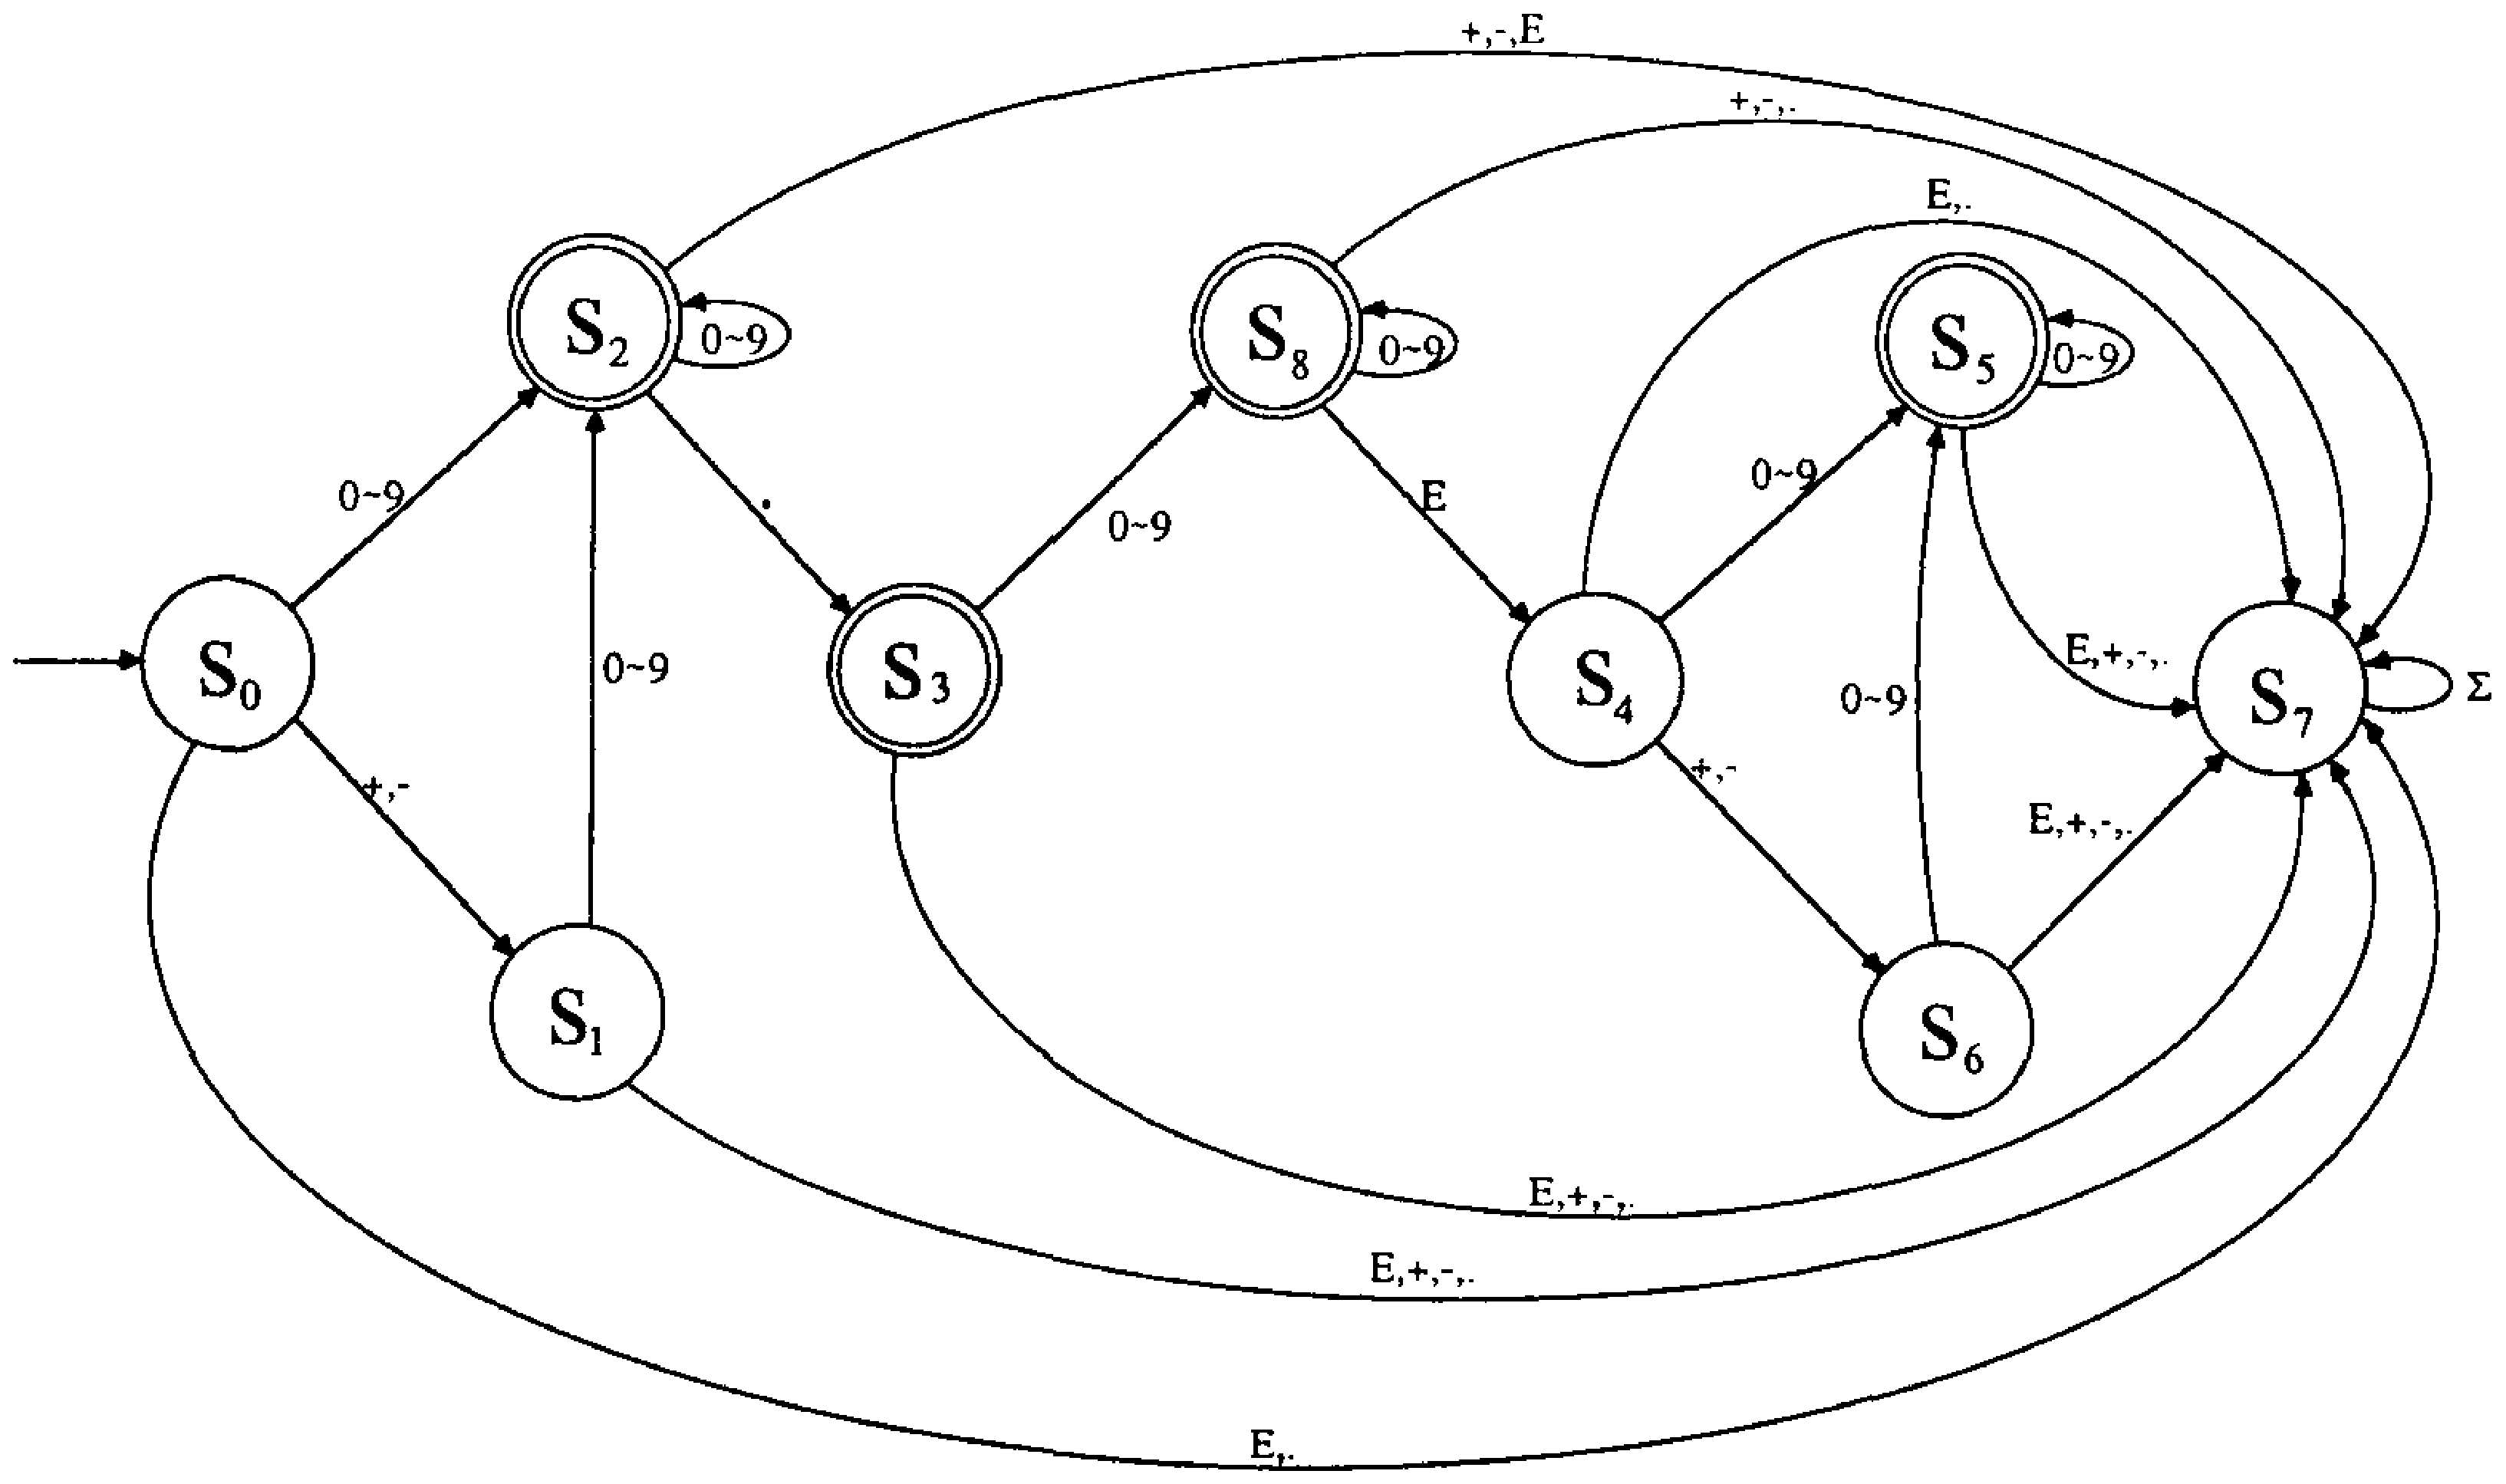
\epsfig{figure=ToFAfigures/fig1-13.eps,width=6.5in}}
\caption{A DFA that recognizes real number constants}\label{fig-1.13}
\end{figure}

For example, let $x = \pmb{3.1415}$:
\begin{align*}
\DBAR(s_0,x) &= \DBAR(s_0,\pmb{3.1415}) \\
&= \DBAR(\delta(s_0,\pmb{3}),\pmb{.1415}) \\
&= \DBAR(s_2,\pmb{.1415}) \\
&= \DBAR(\delta(s_2,\pmb{.}),\pmb{1415}) \\
&= \DBAR(s_3,\pmb{1415}) \\
&= \DBAR(\delta(s_3,\pmb{1}),\pmb{415}) \\
&= \DBAR(s_8,\pmb{415}) \\
&= \DBAR(\delta(s_8,\pmb{4}),\pmb{15}) \\
&= \DBAR(s_8,\pmb{15}) \\
&= \DBAR(\delta(s_8,\pmb{1}),\pmb{5}) \\
&= \DBAR(s_8,\pmb{5}) \\
&= \delta(s_8,\pmb{5}) \\
&= s_8
\end{align*}
$s_8 \in F$, and therefore $\pmb{3.1415}\in L(R)$.

While many important classes of strings such as numerical constants (Example
1.11) and identifiers (Example 1.9) are FAD, not all languages
that can be described by BNF can be recognized by DFAs. These limitations will
be investigated in Chapters \ref{ch-8} and \ref{ch-9}, and a more capable type
of automaton will be defined in Chapter \ref{ch-10}.

\section{Circuit Implementation of Finite Automata}\label{sec-1.4}\index{finite automaton!circuit implementation}

Now that we have described the mathematical nature of deterministic finite
automata, let us turn to the physical implementation of such devices. We will
investigate the sort of physical components that actually go into the ``brain''
of, say, a vending machine. Recall that the basic building blocks of digital
logic circuits are {\emph{\Index{logic gates}}; using $\pmb{0}$ or {\bf False}
to represent a low voltage (ground) and $\pmb{1}$ or {\bf True} to represent a
higher voltage (often +5 volts), the basic gates have the truth tables shown in
Figure \ref{fig-1.14}.

Since our DFA will examine one letter at a time, we will generally need some
type of timing mechanism, which will be regulated by a
\emph{\Index{clock pulse}}; we will read one letter per pulse and allow enough
interim time for transient signals to propagate through our network as we change
states and move to the next letter on the input tape. The clock pulse will
alternate between high and low voltages, as shown in Figure \ref{fig-1.15}.
For applications such as vending machines, the periodic clock pulse would be
replaced by a device that pulsed whenever a new input (such as the insertion of
a coin) was detected.

% Figure 1.14
\begin{figure}
\centerline{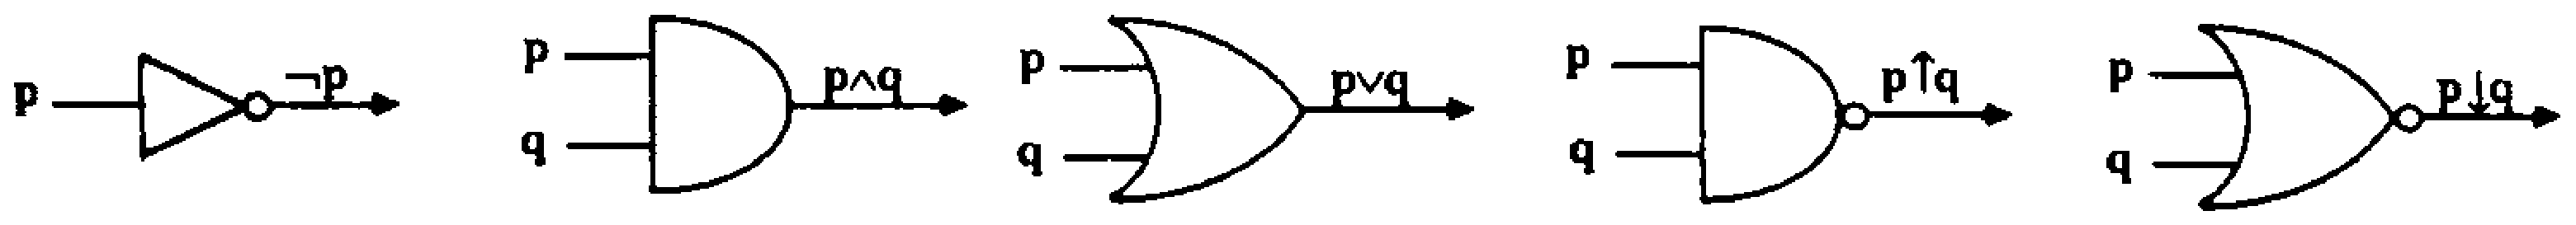
\epsfig{figure=ToFAfigures/fig1-14.eps,width=5.7in}}
\begin{center}
\begin{tabular}{ccccc}
%\fbox{IMAGE} & \fbox{IMAGE} & \fbox{IMAGE} & \fbox{IMAGE} & \fbox{IMAGE} \\
NOT gate & AND gate & OR gate & NAND gate & NOR gate \\
{
\begin{tabular}[b]{c|c}
$p$ & $\neg p$ \\
\hline
$\pmb{1}$ & $\pmb{0}$ \\
$\pmb{0}$ & $\pmb{1}$
\end{tabular}
} & {
\begin{tabular}{cc|c}
$p$ & $q$ & $p\wedge q$ \\
\hline
$\pmb{1}$ & $\pmb{1}$ & $\pmb{1}$ \\
$\pmb{1}$ & $\pmb{0}$ & $\pmb{0}$ \\
$\pmb{0}$ & $\pmb{1}$ & $\pmb{0}$ \\
$\pmb{0}$ & $\pmb{0}$ & $\pmb{0}$
\end{tabular}
} & {
\begin{tabular}{cc|c}
$p$ & $q$ & $p\vee q$ \\
\hline
$\pmb{1}$ & $\pmb{1}$ & $\pmb{1}$ \\
$\pmb{1}$ & $\pmb{0}$ & $\pmb{1}$ \\
$\pmb{0}$ & $\pmb{1}$ & $\pmb{1}$ \\
$\pmb{0}$ & $\pmb{0}$ & $\pmb{0}$
\end{tabular}
} & {
\begin{tabular}{cc|c}
$p$ & $q$ & $p \uparrow q$ \\
\hline
$\pmb{1}$ & $\pmb{1}$ & $\pmb{0}$ \\
$\pmb{1}$ & $\pmb{0}$ & $\pmb{1}$ \\
$\pmb{0}$ & $\pmb{1}$ & $\pmb{1}$ \\
$\pmb{0}$ & $\pmb{0}$ & $\pmb{1}$
\end{tabular}
} & {
\begin{tabular}{cc|c}
$p$ & $q$ & $p \downarrow q$ \\
\hline
$\pmb{1}$ & $\pmb{1}$ & $\pmb{0}$ \\
$\pmb{1}$ & $\pmb{0}$ & $\pmb{0}$ \\
$\pmb{0}$ & $\pmb{1}$ & $\pmb{0}$ \\
$\pmb{0}$ & $\pmb{0}$ & $\pmb{1}$
\end{tabular}
}
\end{tabular}
\end{center}
\caption{Common logic gates and their truth tables}\label{fig-1.14}
\end{figure}

% Figure 1.15
\begin{figure}
\centerline{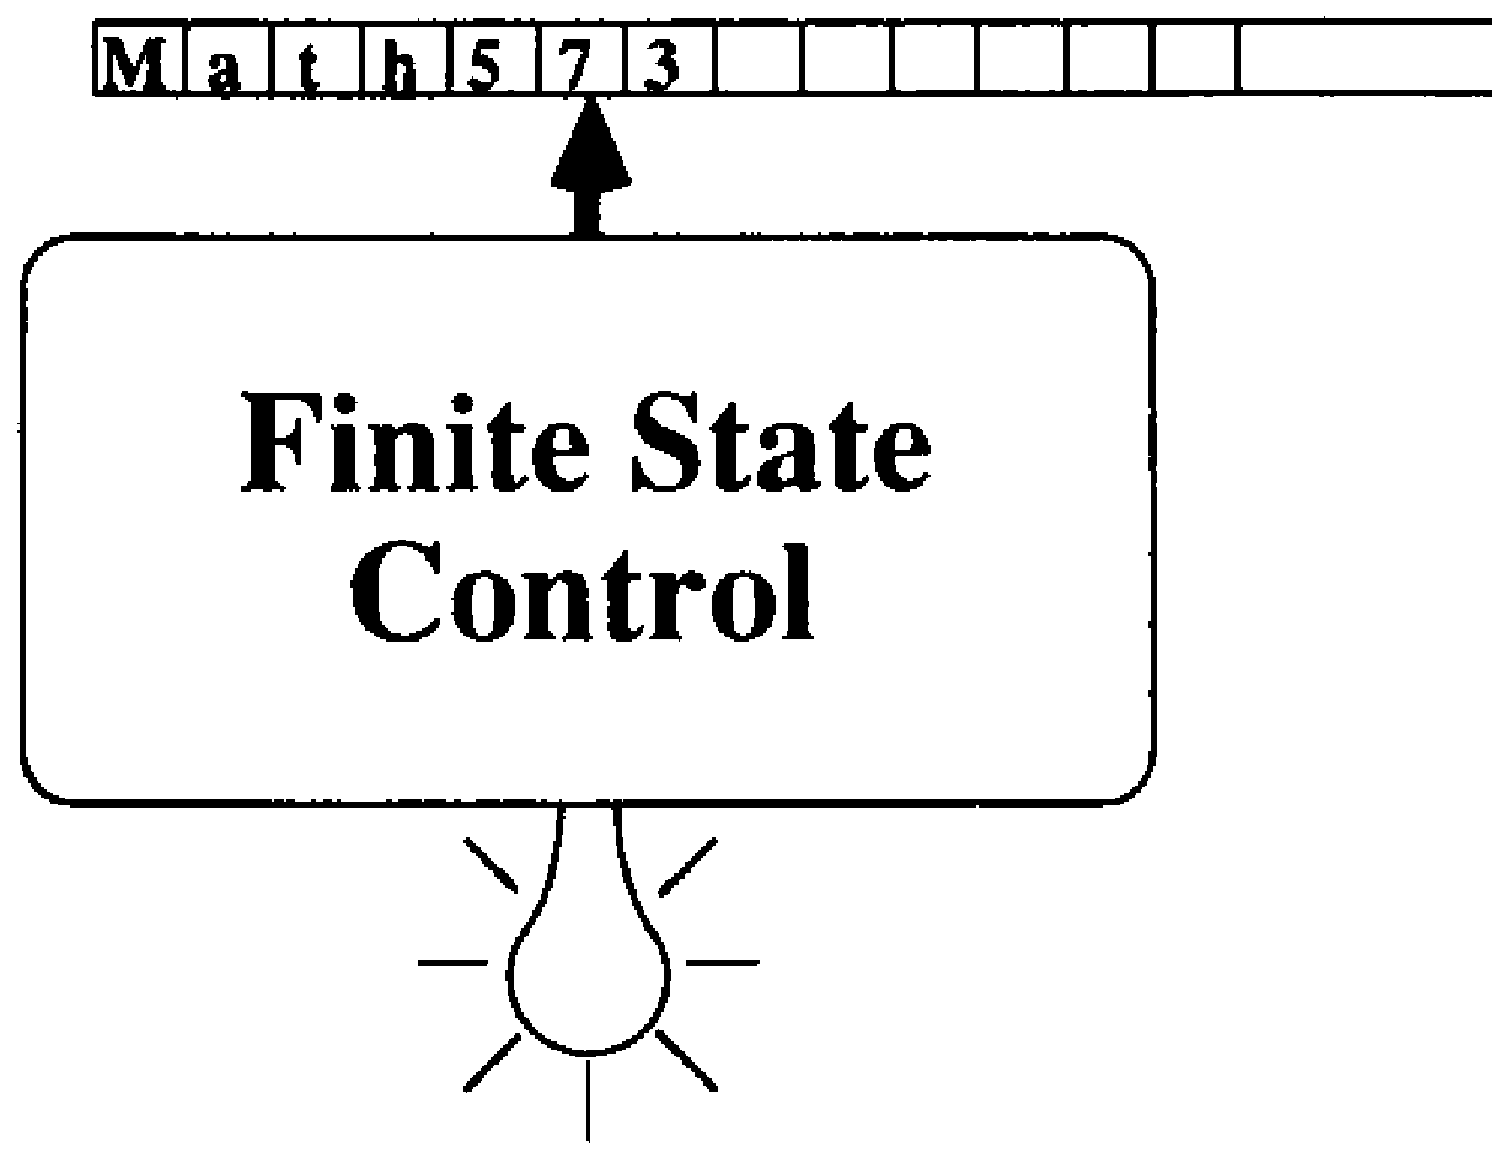
\epsfig{figure=ToFAfigures/fig1-1.eps,width=4in}}
\caption{A typical clock pulse pattern for latched circuits}\label{fig-1.15}
\end{figure}

We need to retain the present status of the network (current state, letter, and
so forth) as we move on to the next input symbol. This is achieved through the
use of a \emph{\Index{D flip-flop}} (D stands for data or delay), which uses
NAND gates and the clock signal to store the current value of, say, \emph{$p'$},
between clock pulses. The symbol for a D flip-flop (sometimes called a
\emph{\Index{latch}}) is shown in Figure \ref{fig-1.16}, along with the actual
gates that comprise the circuit.

The output, $p$ and $\neg p$, will reflect the value of the input signal $p'$
\emph{only} after the high clock pulse is received and will retain that value after the
clock drops to low (even if $p'$ subsequently changes) until the next clock
pulse comes along, at which time the output will reflect the new current value
of $p'$. This is best illustrated by referring to the NAND truth table and
tracing the changes in the circuit. Begin with clock $= p = p' = \pmb{0}$ and 
$\neg p = \pmb{1}$, and verify that the circuit is stable. Now assume that $p'$
changes to $\pmb{1}$, and note that, although some internal values may change,
$p$ and $\neg p$ remain at $\pmb{0}$ and $\pmb{1}$, respectively; the old value
of $p'$ has been ``remembered'' by the D flip-flop. Contrast this with the
behavior when we strobe the clock: assume that the clock now also changes to
$\pmb{1}$ so that we now have clock $=p=p'=\pmb{1}$, and $p=\pmb{0}$. When the
signal propagates through the network, we find that $p$ and $\neg p$ have
changed to reflect the new value of $p'$; clock $=p=p'=\pmb{1}$, and $\neg p=
\pmb{0}$.

We will also have to represent the letters of our input alphabet by high and low
voltages (that is, combinations of $\pmb{0}$s and $\pmb{1}$s). The \index{ASCII alphabet}ASCII alphabet,
for example, is quite naturally represented by 8 bits, 
$\pmb{a}_1\pmb{a}_2\pmb{a}_3\pmb{a}_4\pmb{a}_5\pmb{a}_6\pmb{a}_7\pmb{a}_8$,
where $\pmb{B}$, for example, has the bit pattern $\pmb{01000010}$ (binary 66).
One of these bit patterns should be reserved for indicating the end of our input
string \<EOS\>. Our convention will be to reserve binary zero for this role,
which means our ASCII end of string symbol would be $\pmb{00000000}$ (or NULL).
In actual applications using the ASCII alphabet, however, a more appropriate
choice for \<EOS\> might be $\pmb{00001101}$ (a carriage return) or
$\pmb{00001010}$ (a line feed) or $\pmb{00100000}$ (a space).

% Figure 1.16
\begin{figure}
\centerline{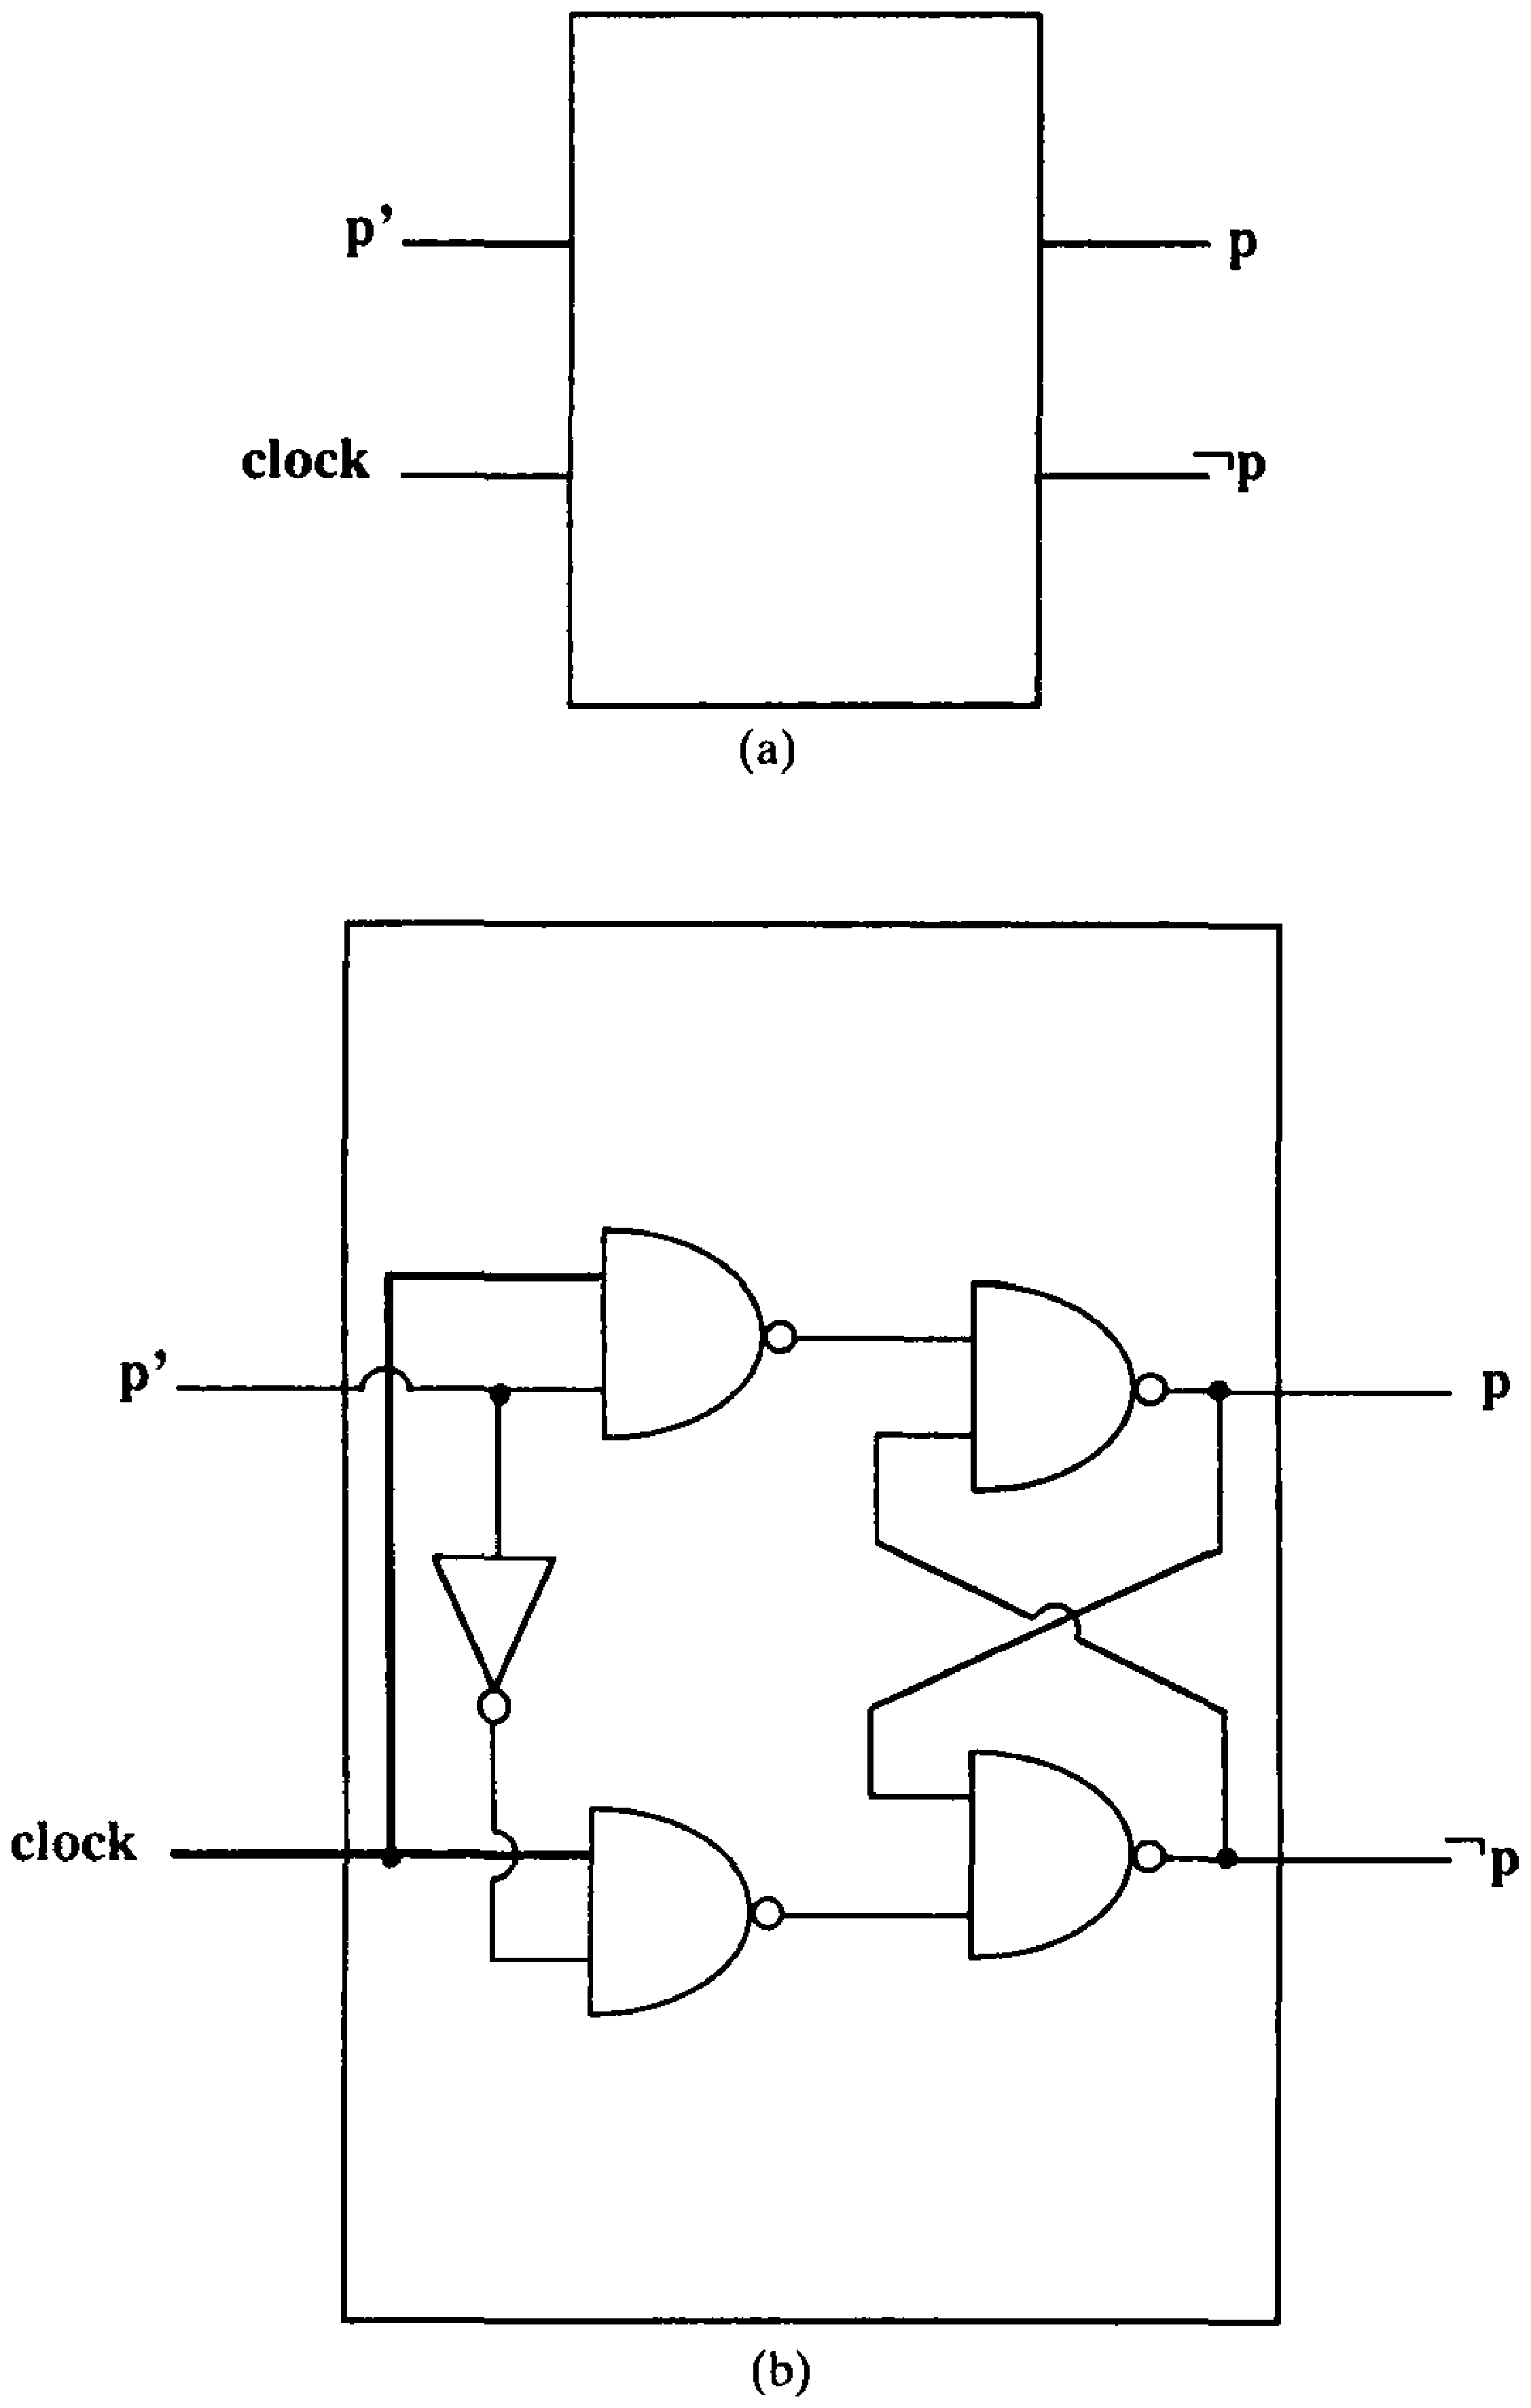
\epsfig{figure=ToFAfigures/fig1-16.eps,width=2.5in}}
\caption{(a) A data flip-flop or latch (b) The circuitry for a D flip-flop}\label{fig-1.16}
\end{figure}

Our alphabets are likely to be far smaller than the ASCII character set, and we
will hence need fewer than 8 bits of information to encode our letters. For
example, if $\Sigma = \{\pmb{b},\pmb{c}\}$, 2 bits, $\pmb{a}_1$ and $\pmb{a}_2$,
will suffice. Our choice of encoding could be $\pmb{00}$ = \<EOS\>, $\pmb{01}=
\pmb{b}$, $\pmb{10}=\pmb{c}$, and $\pmb{11}$ is unused.

In a similar fashion, we must encode state names. A machine with
$S = \{r_0,r_1,r_2,r_3,r_4,r_5\}$ would need 3 bits (denoted by $t_1$, $t_2$,
and $t_3$) to represent the six states. The most natural encoding would be
$r_0 = \pmb{000}$, $r_1 = \pmb{001}$, $r_2 = \pmb{010}$, $r_3 = \pmb{011}$,
$r_4 = \pmb{100}$, and $r_5 = \pmb{101}$, with the combinations $\pmb{110}$ and
$\pmb{111}$ left unused.

Finally, a mechanism for differentiating between final and nonfinal states
must be implemented (although this need not be engaged until the \<EOS\> symbol
is encountered). Recall that we must illuminate the ``acceptance light'' if the
machine terminates in a final state and leave it unlit if the string on the
input tape is instead rejected by the DFA. A second ``rejection light'' can be
added to the physical model, and exactly one of the two will light when \<EOS\>
is scanned by the input head.

% Example 1.12
\subsection*{Example 1.12}

When building a logical circuit from the definition of a DFA, we will find it
convenient to treat \<EOS\> as an input symbol, and define the state transition
function for it by $(\forall s \in S)(\delta(s_1,\<EOS\>) = s)$. Thus, the DFA
in Figure \ref{fig-1.17}a should be thought of as shown in Figure
\ref{fig-1.17}b. As we have only two states, a single state bit will suffice,
representing $s_0$ by $t_1=\pmb{0}$ and $s_1$ by $t_1=\pmb{1}$. Since $\Sigma=
\{\pmb{b},\pmb{c}\}$, we will again use 2 bits, $\pmb{a}_1$ and $\pmb{a}_2$, to
represent the input symbols. As before, $\pmb{00}$ = \<EOS\>, $\pmb{01} = b$,
$\pmb{10} = c$, and $\pmb{11}$ is unused.

% Figure 1.17
\begin{figure}
\centerline{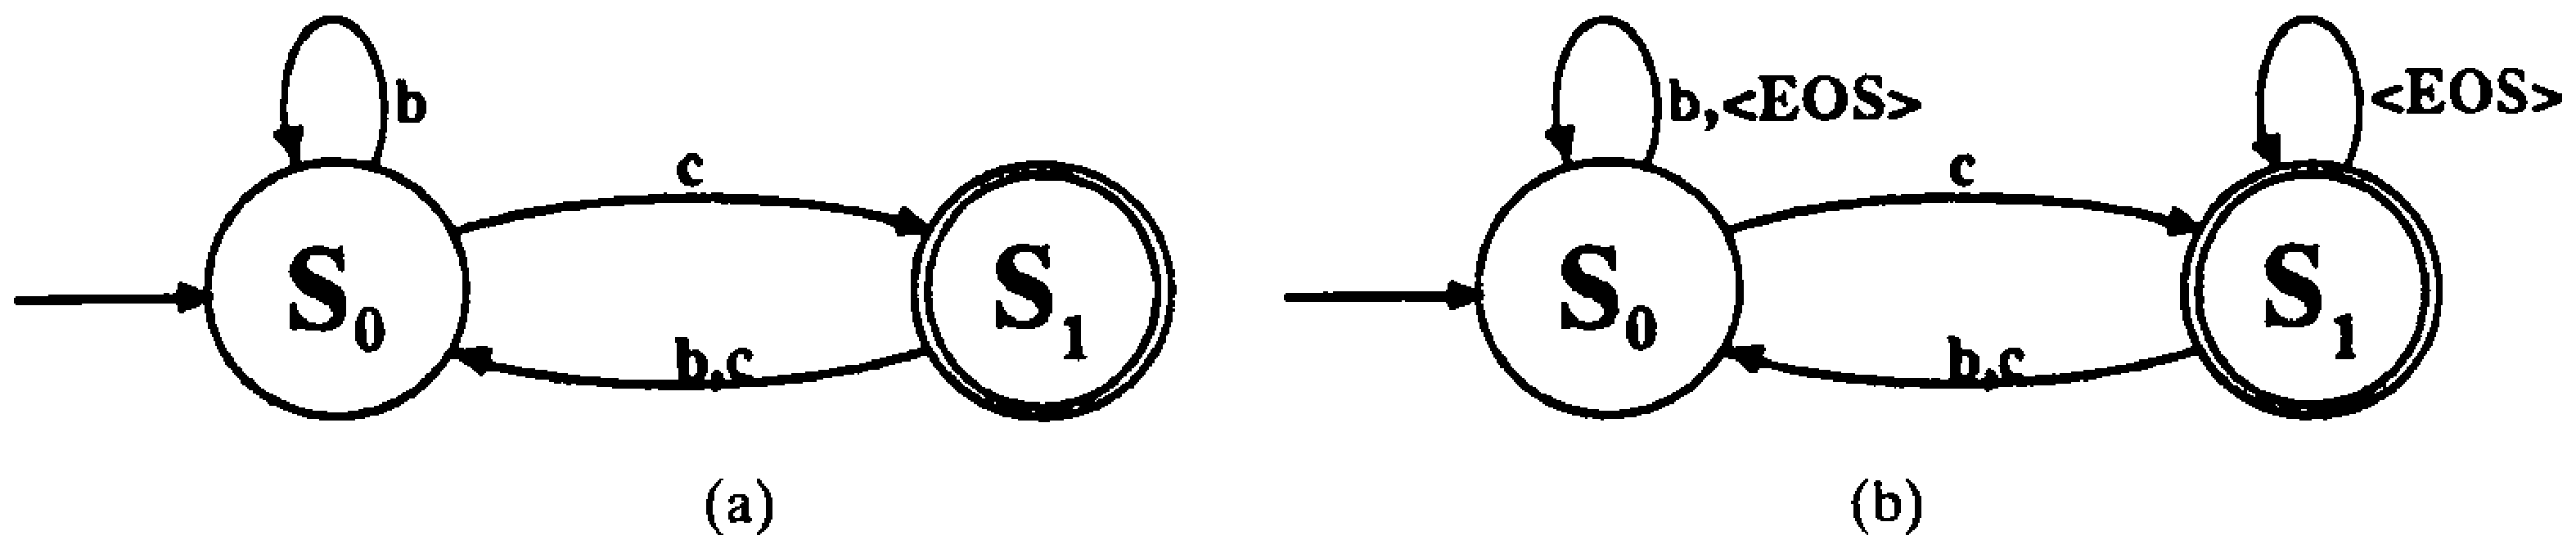
\epsfig{figure=ToFAfigures/fig1-17.eps,width=5in}}
\caption{(a) The DFA discussed in Example 1.12 (b) The expanded state transition
diagram for the DFA implemented in Figure \ref{fig-1.18}}\label{fig-1.17}
\end{figure}

Determining the state transition function will require knowledge of the current
state (represented by the status of $t_1$) and the current input symbol
(represented by the pair of bits $a_1$ and $a_2$). These three input values will
allow the next state $t_1'$ to be calculated. From the $\delta$ function, we
know that
\begin{align*}
\delta(s_0,\pmb{b}) = s_0 \\
\delta(s_0,\pmb{c}) = s_1 \\
\delta(s_1,\pmb{b}) = s_0 \\
\delta(s_1,\pmb{c}) = s_0
\end{align*}
These specifications correspond to the following four rows of the truth table
for $t_1'$:

\begin{center}\begin{tabular}{ccc}
{
\begin{tabular}{ccc|c}
$t_1$ & $\pmb{a}_1$ & $\pmb{a}_2$ & $t_1'$ \\
\hline
$\pmb{0}$ & $\pmb{0}$ & $\pmb{1}$ & $\pmb{0}$ \\
$\pmb{0}$ & $\pmb{1}$ & $\pmb{0}$ & $\pmb{1}$ \\
$\pmb{1}$ & $\pmb{0}$ & $\pmb{1}$ & $\pmb{0}$ \\
$\pmb{1}$ & $\pmb{1}$ & $\pmb{0}$ & $\pmb{0}$
\end{tabular}
} & {
which represents
} & {
\begin{tabular}{cl|c}
$t_1$ & $\pmb{a}_1\ \ \pmb{a}_2$ & $t_1'$ \\
\hline
$s_{\pmb{0}}$ & $\underline{\pmb{0}\ \ \ \ \pmb{1}} = \pmb{b}$ & $s_{\pmb{0}}$ \\
$s_{\pmb{0}}$ & $\underline{\pmb{1}\ \ \ \ \pmb{0}} = \pmb{c}$ & $s_{\pmb{1}}$ \\
$s_{\pmb{1}}$ & $\underline{\pmb{0}\ \ \ \ \pmb{1}} = \pmb{b}$ & $s_{\pmb{0}}$ \\
$s_{\pmb{1}}$ & $\underline{\pmb{1}\ \ \ \ \pmb{0}} = \pmb{c}$ & $s_{\pmb{0}}$
\end{tabular}
}
\end{tabular}\end{center}

Adding the state transitions for \<EOS\> and using * to represent the
outcome for the two rows corresponding to the unused combination $\pmb{a}_1
\pmb{a}_2=\pmb{11}$ fills out the eight rows of the complete truth table, as
shown in Table \ref{tbl-1.2}.

% Table 1.2
\begin{table}[h]\caption{}\label{tbl-1.2}
\begin{center}
\begin{tabular}{ccc|c}
$t_1$ & $\pmb{a}_1$ & $\pmb{a}_2$ & $t_1'$ \\
\hline
$\pmb{0}$ & $\pmb{0}$ & $\pmb{0}$ & $\pmb{0}$ \\
$\pmb{0}$ & $\pmb{0}$ & $\pmb{1}$ & $\pmb{0}$ \\
$\pmb{0}$ & $\pmb{1}$ & $\pmb{0}$ & $\pmb{1}$ \\
$\pmb{0}$ & $\pmb{1}$ & $\pmb{1}$ & * \\
$\pmb{1}$ & $\pmb{0}$ & $\pmb{0}$ & $\pmb{1}$ \\
$\pmb{1}$ & $\pmb{0}$ & $\pmb{1}$ & $\pmb{0}$ \\
$\pmb{1}$ & $\pmb{1}$ & $\pmb{0}$ & $\pmb{0}$ \\
$\pmb{1}$ & $\pmb{1}$ & $\pmb{1}$ & *
\end{tabular}
\end{center}
\end{table}

If we arbitrarily assume that the two don't-care combinations (*) are zero, the
principle disjunctive normal form of $t_1'$ contains just two terms:
$(\neg t_1\wedge\pmb{a}_1\wedge\neg\pmb{a}_2)\vee(t_1\wedge\neg\pmb{a}_1\wedge
\neg\pmb{a}_2)$. It is profitable to reassign the don't-care value in the fourth
row to $\pmb{1}$, since the expression can then be shortened to $(\neg t_1\wedge
\pmb{a}_1)\vee(t_1\wedge\neg\pmb{a}_1\wedge\neg\pmb{a}_2)$ by applying standard
techniques for minimizing Boolean functions. Incorporating this into a feedback
loop with a D flip-flop provides the heart of the digital logic circuit
representing the DFA, as shown in Figure \ref{fig-1.18}.

% Figure 1.18
\begin{figure}
\centerline{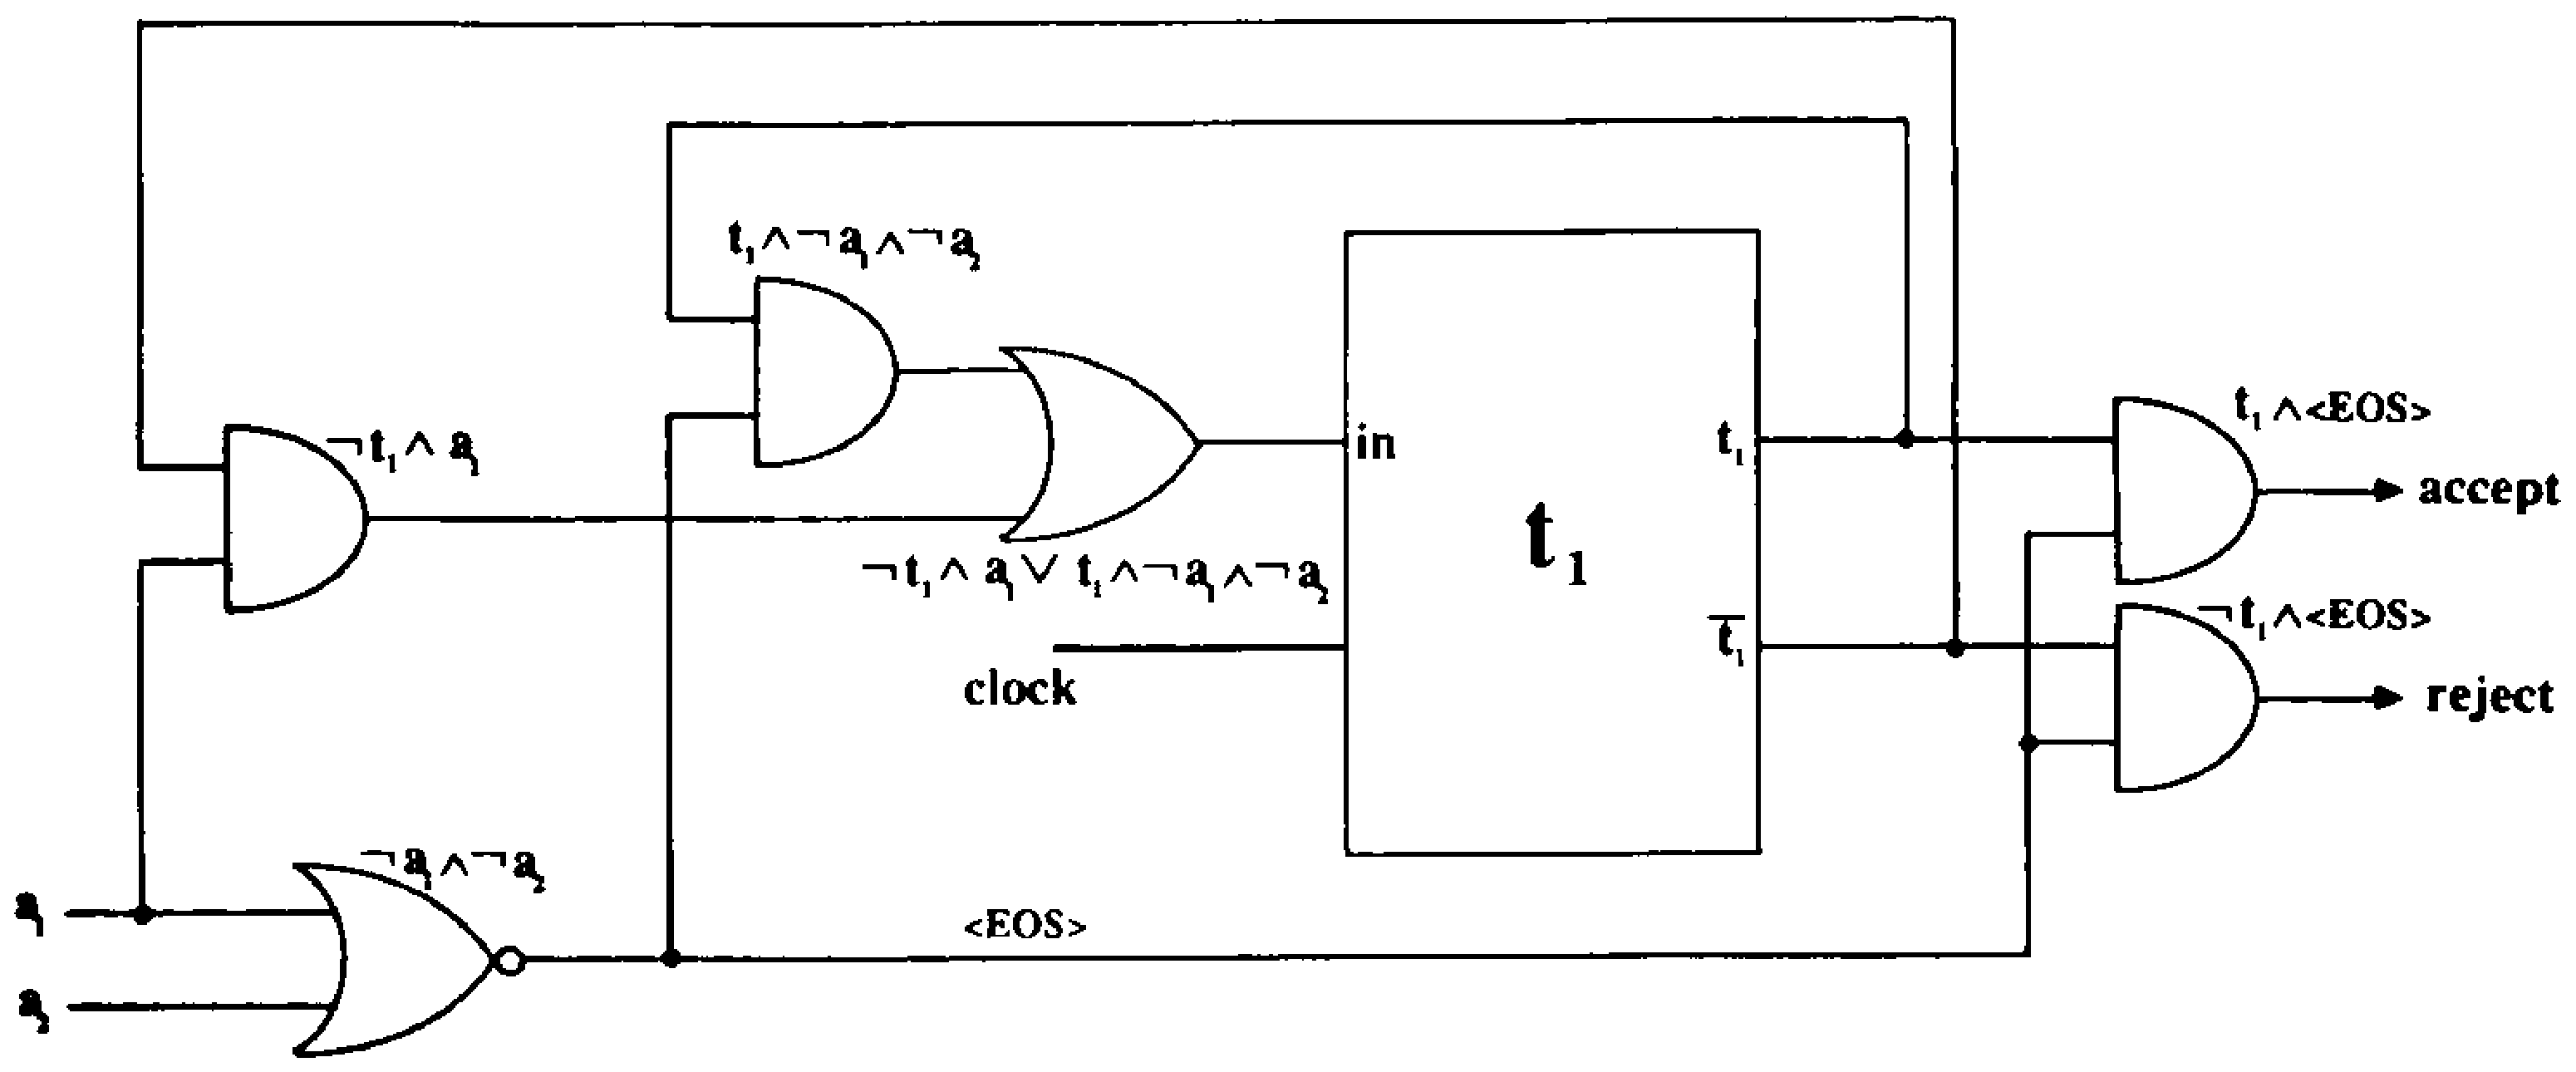
\epsfig{figure=ToFAfigures/fig1-18.eps,width=6in}}
\caption{The circuitry implementing the DFA discussed in Example 1.12}\label{fig-1.18}
\end{figure}

The accept portion of the circuitry\index{accept circuitry} ensures that we do not indicate acceptance
when passing through the final state; it is only activated when we are in a
final state while scanning the \<EOS\> symbol. Similarly, the reject circuitry
can only be activated when the \<EOS\> symbol is encountered. When there are
several final states, this part of the circuitry becomes correspondingly more
complex. It is instructive to follow the effect a string such as $\pmb{bcc}$ has
on the above circuit. Define $\pmb{a}_i(j)$ as the $j$th value the bit $\pmb{a}_i$
takes on as the string $\pmb{bcc}$ is processed; that is, $\pmb{a}_i(j)$ is the
value of $\pmb{a}_i$ during the $j$th clock pulse. We then have
\begin{center}\begin{tabular}{r@{ $=$ }l@{$\qquad$}r@{ $=$ }l@{$\qquad\Rightarrow$ }l}
$\pmb{a}_1(1)$ & $\pmb{0}$ & $\pmb{a}_2(1)$ & $\pmb{1}$ & $\pmb{b}$ \\
$\pmb{a}_1(2)$ & $\pmb{1}$ & $\pmb{a}_2(2)$ & $\pmb{0}$ & $\pmb{c}$ \\
$\pmb{a}_1(3)$ & $\pmb{1}$ & $\pmb{a}_2(3)$ & $\pmb{0}$ & $\pmb{c}$ \\
$\pmb{a}_1(4)$ & $\pmb{0}$ & $\pmb{a}_2(4)$ & $\pmb{0}$ & \<EOS\>
\end{tabular}\end{center}
Trace the circuit through four clock pulses (starting with $t_1=\pmb{0}$), and
observe the current values that $t_1$ assumes, noting that it corresponds to the
appropriate state of the machine as each input symbol is scanned.

Note that a six-state machine would require more and substantially larger
truth tables. Since a state encoding would now need to specify $t_1$, $t_2$, and
$t_3$, three different truth tables (for $t_1'$, $t_2'$, and $t_3'$) must be
constructed to predict the next state transition. More significantly, the input
variables would include $t_1$, $t_2$, $t_3$, $\pmb{a}_1$, and $\pmb{a}_2$,
making each table 32 rows long. Three D flip-flop feedback loops would be
necessary to store the three values $t_1$, $t_2$, and $t_3$.

Also, physical logic circuits of this type have the disconcerting habit of
initializing to some random configuration the first time power is applied to the
network. A true working model would thus need a \emph{reset}\index{reset circuitry} circuit to
initialize each $t_i$ to $\pmb{0}$ in order to ensure that the machine started
in state $s_0$. Slightly more complex set-reset flip-flops can be used to
provide a hardware solution to this problem. However, a simple algorithmic
solution would require the input tape to have a \emph{leading} start-of-string
symbol \<SOS\>. The definition of the state transition function should be
expanded so that scanning the \<SOS\> symbol from any state will automatically
transfer control to $s_0$. We will adopt the convention that \<SOS\> will be
represented by the highest binary code; in ASCII, for example, this would be
$\pmb{11111111}$, while in the preceding example it would be $\pmb{11}$. To
promote uniformity in the exercises, it is suggested that \<SOS\> should always
be given the highest binary code and \<EOS\> be represented by binary zero; as
in the examples given here, the symbols in $\Sigma$ should be numbered
sequentially according to their natural alphabetical order. In a similar
fashion, numbered states should be given their corresponding binary codes. The
reader should note, however, that other encodings might result in less complex
circuitry.

\subsection*{Example 1.13}

As a more complex example of automaton circuitry, consider the DFA displayed in
Figure \ref{fig-1.19}. Two flip-flops $t_1$ and $t_2$ will be necessary to
represent the three states, most naturally encoded as $s_0 = \pmb{00}$, $s_1 =
\pmb{01}$, $s_2 = \pmb{10}$, with $s_3 = \pmb{11}$ unused. Employing both
\<SOS\> and \<EOS\> encodings yields the DFA in Figure \ref{fig-1.20}.

% Figure 1.19
\begin{figure}
\centerline{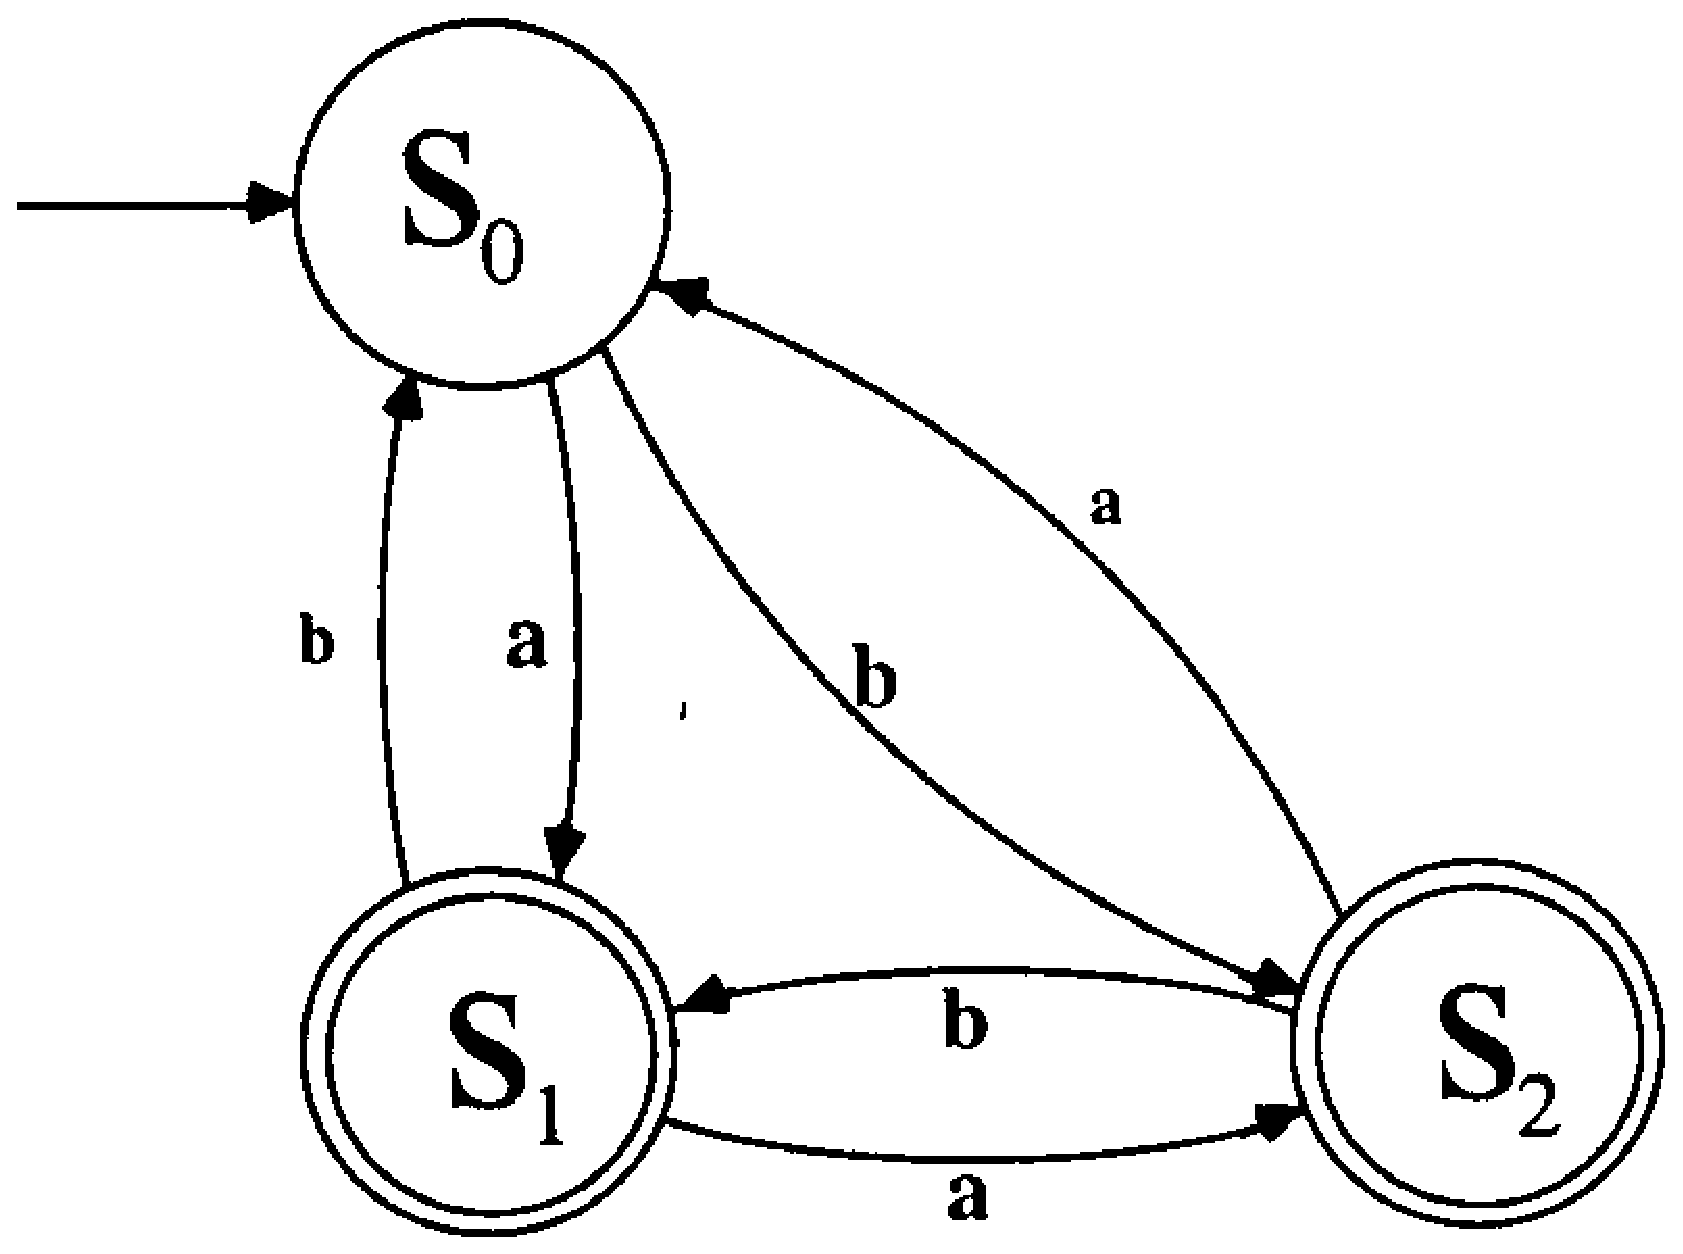
\epsfig{figure=ToFAfigures/fig1-19.eps,width=3in}}
\caption{The DFA discussed in Example 1.13}\label{fig-1.19}
\end{figure}

Note that we must account for the possibility that the circuitry might be
randomly initialized to $t_1=\pmb{1}$ and $t_2=\pmb{1}$; we must ensure that
scanning the \<SOS\> symbol moves us back into the ``real'' part of the machine.
Two bits of information ($\pmb{a}_1$ and $\pmb{a}_2$) are also needed to
describe the input symbols. Following our conventions, we assign \<EOS\> $=
\pmb{00}$, $\pmb{a} = \pmb{01}$, $\pmb{b} = \pmb{10}$, and \<SOS\> $= \pmb{11}$.
The truth table for both the transition function and the conditions for
acceptance is given in Table \ref{tbl-1.3}.

In the first row, $t_1=\pmb{0}$ and $t_2=\pmb{0}$ indicate state $s_0$, while
$\pmb{a}_1=\pmb{0}$ and $\pmb{a}_2=\pmb{0}$ denote the \<EOS\> symbol. Since $\delta(
s_0,\<EOS\>) = s_0$, $t_1'=\pmb{0}$ and $t_2'=\pmb{0}$. We do not want to accept
a string that ends in $s_0$, so {\bf accept}$ = 0$ also. The remaining rows are
determined similarly. The (nonminimized) circuitry for this DFA is shown in
Figure \ref{fig-1.21}.

% Table 1.3
\begin{table}\caption{}\label{tbl-1.3}
\begin{center}
\begin{tabular}{cccc|ccc}
$t_1$ & $t_2$ & $\pmb{a}_1$ & $\pmb{a}_2$ & $t_1'$ & $t_2'$ & {\bf accept} \\
\hline
$\pmb{0}$ & $\pmb{0}$ & $\pmb{0}$ & $\pmb{0}$ & $\pmb{0}$ & $\pmb{0}$ & $\pmb{0}$ \\
$\pmb{0}$ & $\pmb{0}$ & $\pmb{0}$ & $\pmb{1}$ & $\pmb{0}$ & $\pmb{1}$ & $\pmb{0}$ \\
$\pmb{0}$ & $\pmb{0}$ & $\pmb{1}$ & $\pmb{0}$ & $\pmb{1}$ & $\pmb{0}$ & $\pmb{0}$ \\
$\pmb{0}$ & $\pmb{0}$ & $\pmb{1}$ & $\pmb{1}$ & $\pmb{0}$ & $\pmb{0}$ & $\pmb{0}$ \\
$\pmb{0}$ & $\pmb{1}$ & $\pmb{0}$ & $\pmb{0}$ & $\pmb{0}$ & $\pmb{1}$ & $\pmb{1}$ \\
$\pmb{0}$ & $\pmb{1}$ & $\pmb{0}$ & $\pmb{1}$ & $\pmb{1}$ & $\pmb{0}$ & $\pmb{0}$ \\
$\pmb{0}$ & $\pmb{1}$ & $\pmb{1}$ & $\pmb{0}$ & $\pmb{0}$ & $\pmb{0}$ & $\pmb{0}$ \\
$\pmb{0}$ & $\pmb{1}$ & $\pmb{1}$ & $\pmb{1}$ & $\pmb{0}$ & $\pmb{0}$ & $\pmb{0}$ \\
$\pmb{1}$ & $\pmb{0}$ & $\pmb{0}$ & $\pmb{0}$ & $\pmb{1}$ & $\pmb{0}$ & $\pmb{1}$ \\
$\pmb{1}$ & $\pmb{0}$ & $\pmb{0}$ & $\pmb{1}$ & $\pmb{0}$ & $\pmb{0}$ & $\pmb{0}$ \\
$\pmb{1}$ & $\pmb{0}$ & $\pmb{1}$ & $\pmb{0}$ & $\pmb{0}$ & $\pmb{1}$ & $\pmb{0}$ \\
$\pmb{1}$ & $\pmb{0}$ & $\pmb{1}$ & $\pmb{1}$ & $\pmb{0}$ & $\pmb{0}$ & $\pmb{0}$ \\
$\pmb{1}$ & $\pmb{1}$ & $\pmb{0}$ & $\pmb{0}$ & * & * & * \\
$\pmb{1}$ & $\pmb{1}$ & $\pmb{0}$ & $\pmb{1}$ & * & * & * \\
$\pmb{1}$ & $\pmb{1}$ & $\pmb{1}$ & $\pmb{0}$ & * & * & * \\
$\pmb{1}$ & $\pmb{1}$ & $\pmb{1}$ & $\pmb{1}$ & $\pmb{0}$ & $\pmb{0}$ & $\pmb{0}$
\end{tabular}
\end{center}
\end{table}
\

% Figure 1.20
\begin{figure}
\centerline{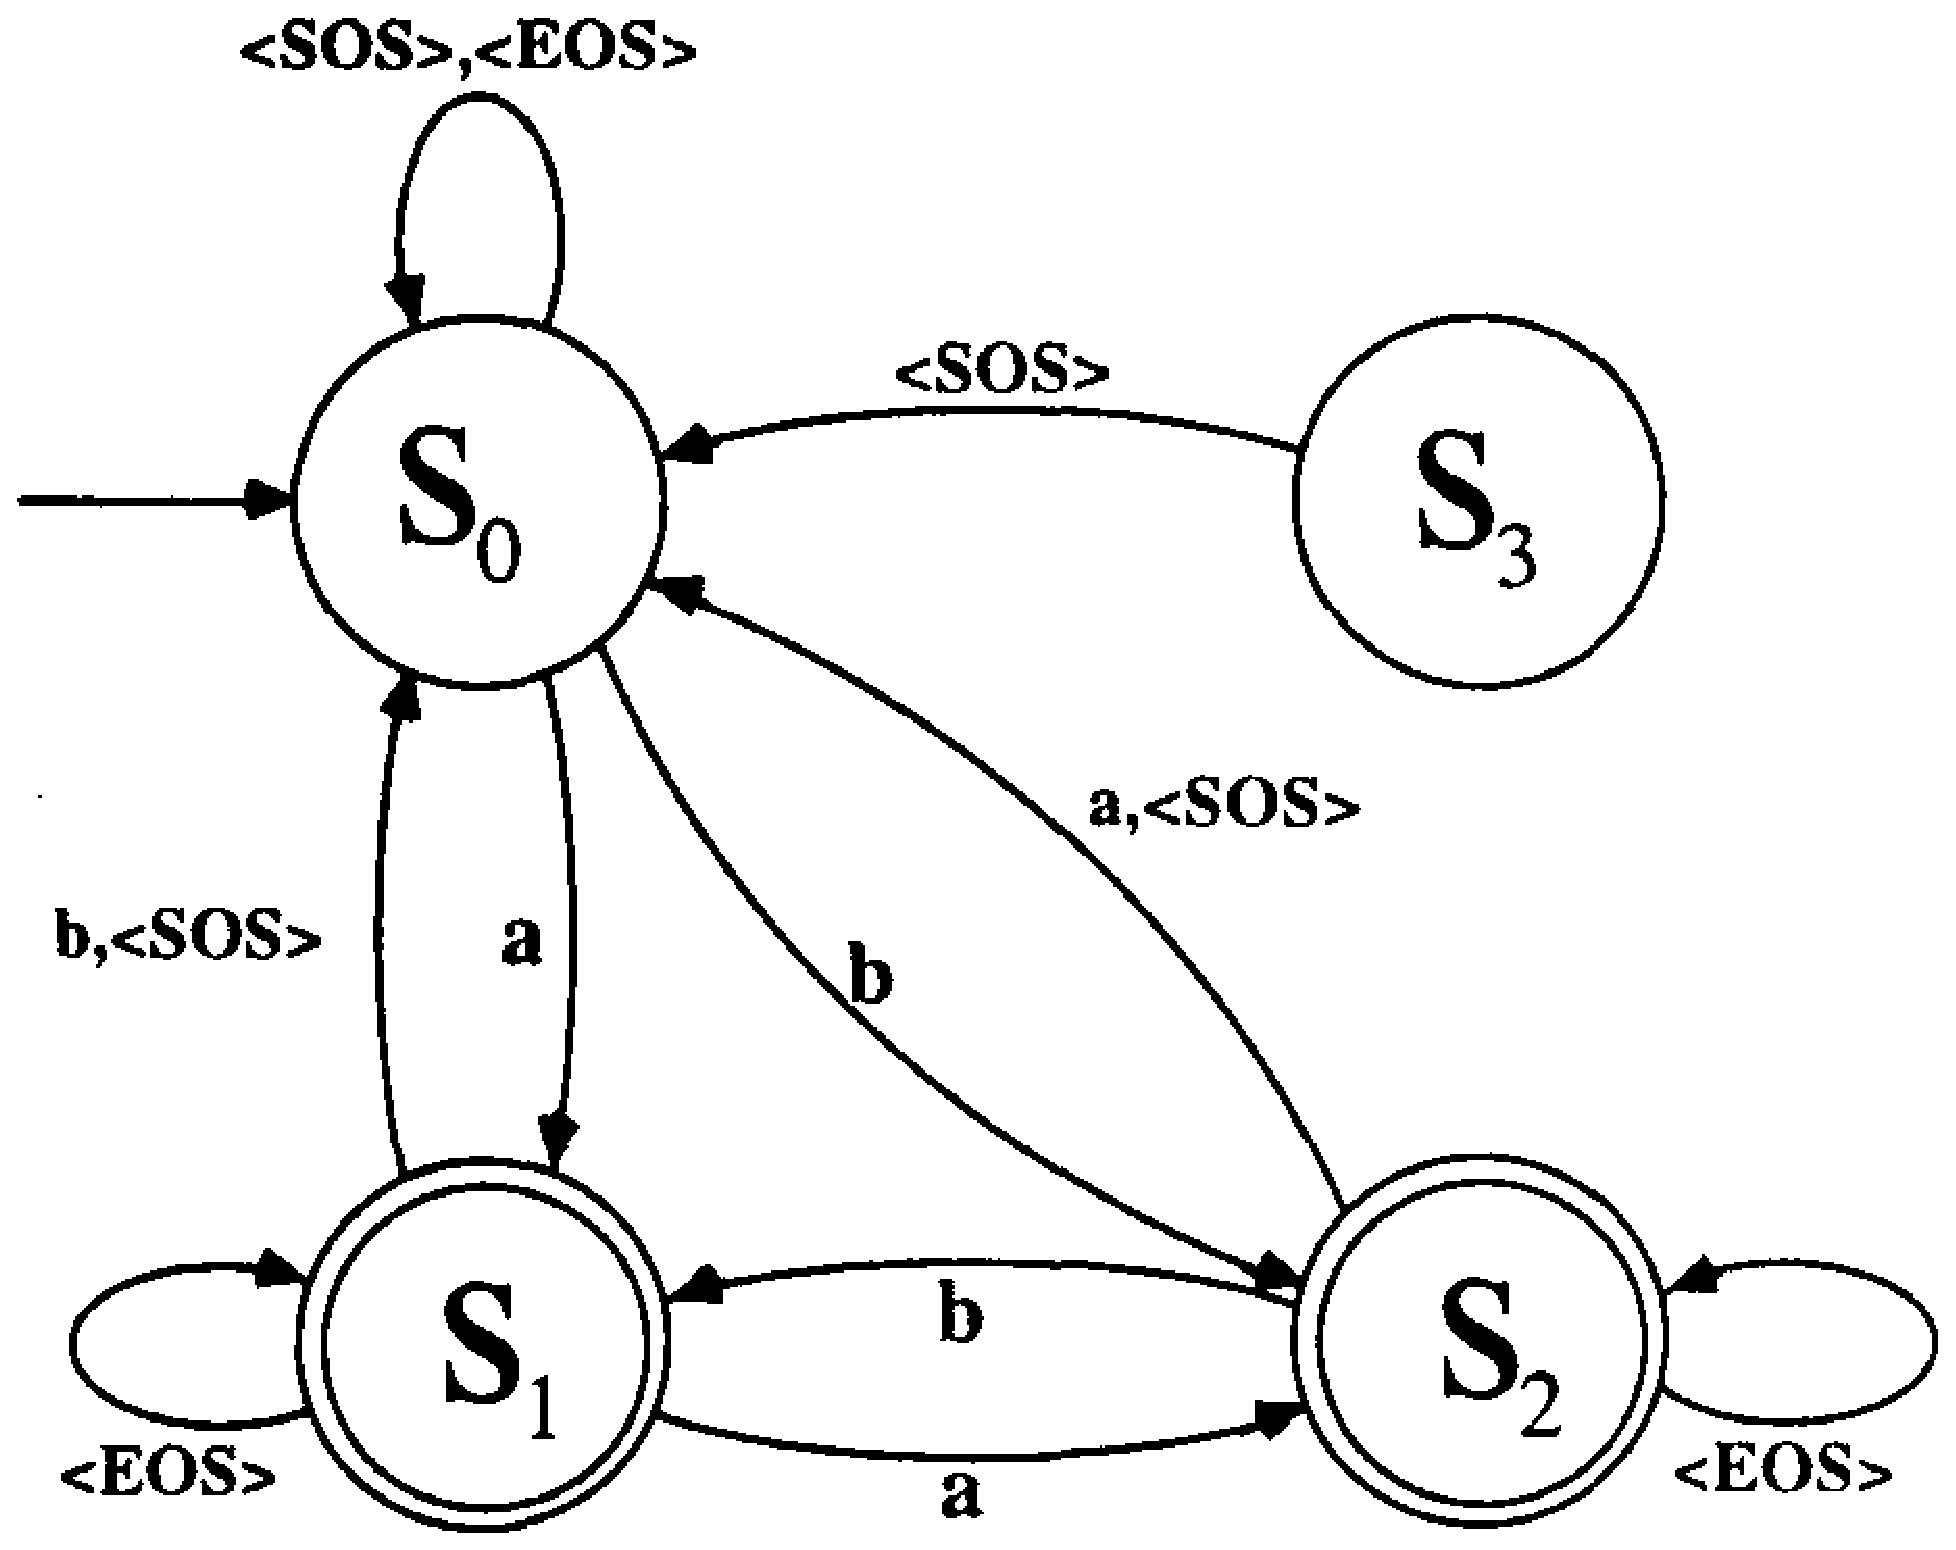
\epsfig{figure=ToFAfigures/fig1-20.eps,width=3.5in}}
\caption{The expanded state transition diagram for the DFA implemented in Figure
\ref{fig-1.21}}\label{fig-1.20}
\end{figure}

% Figure 1.21
\begin{figure}
\centerline{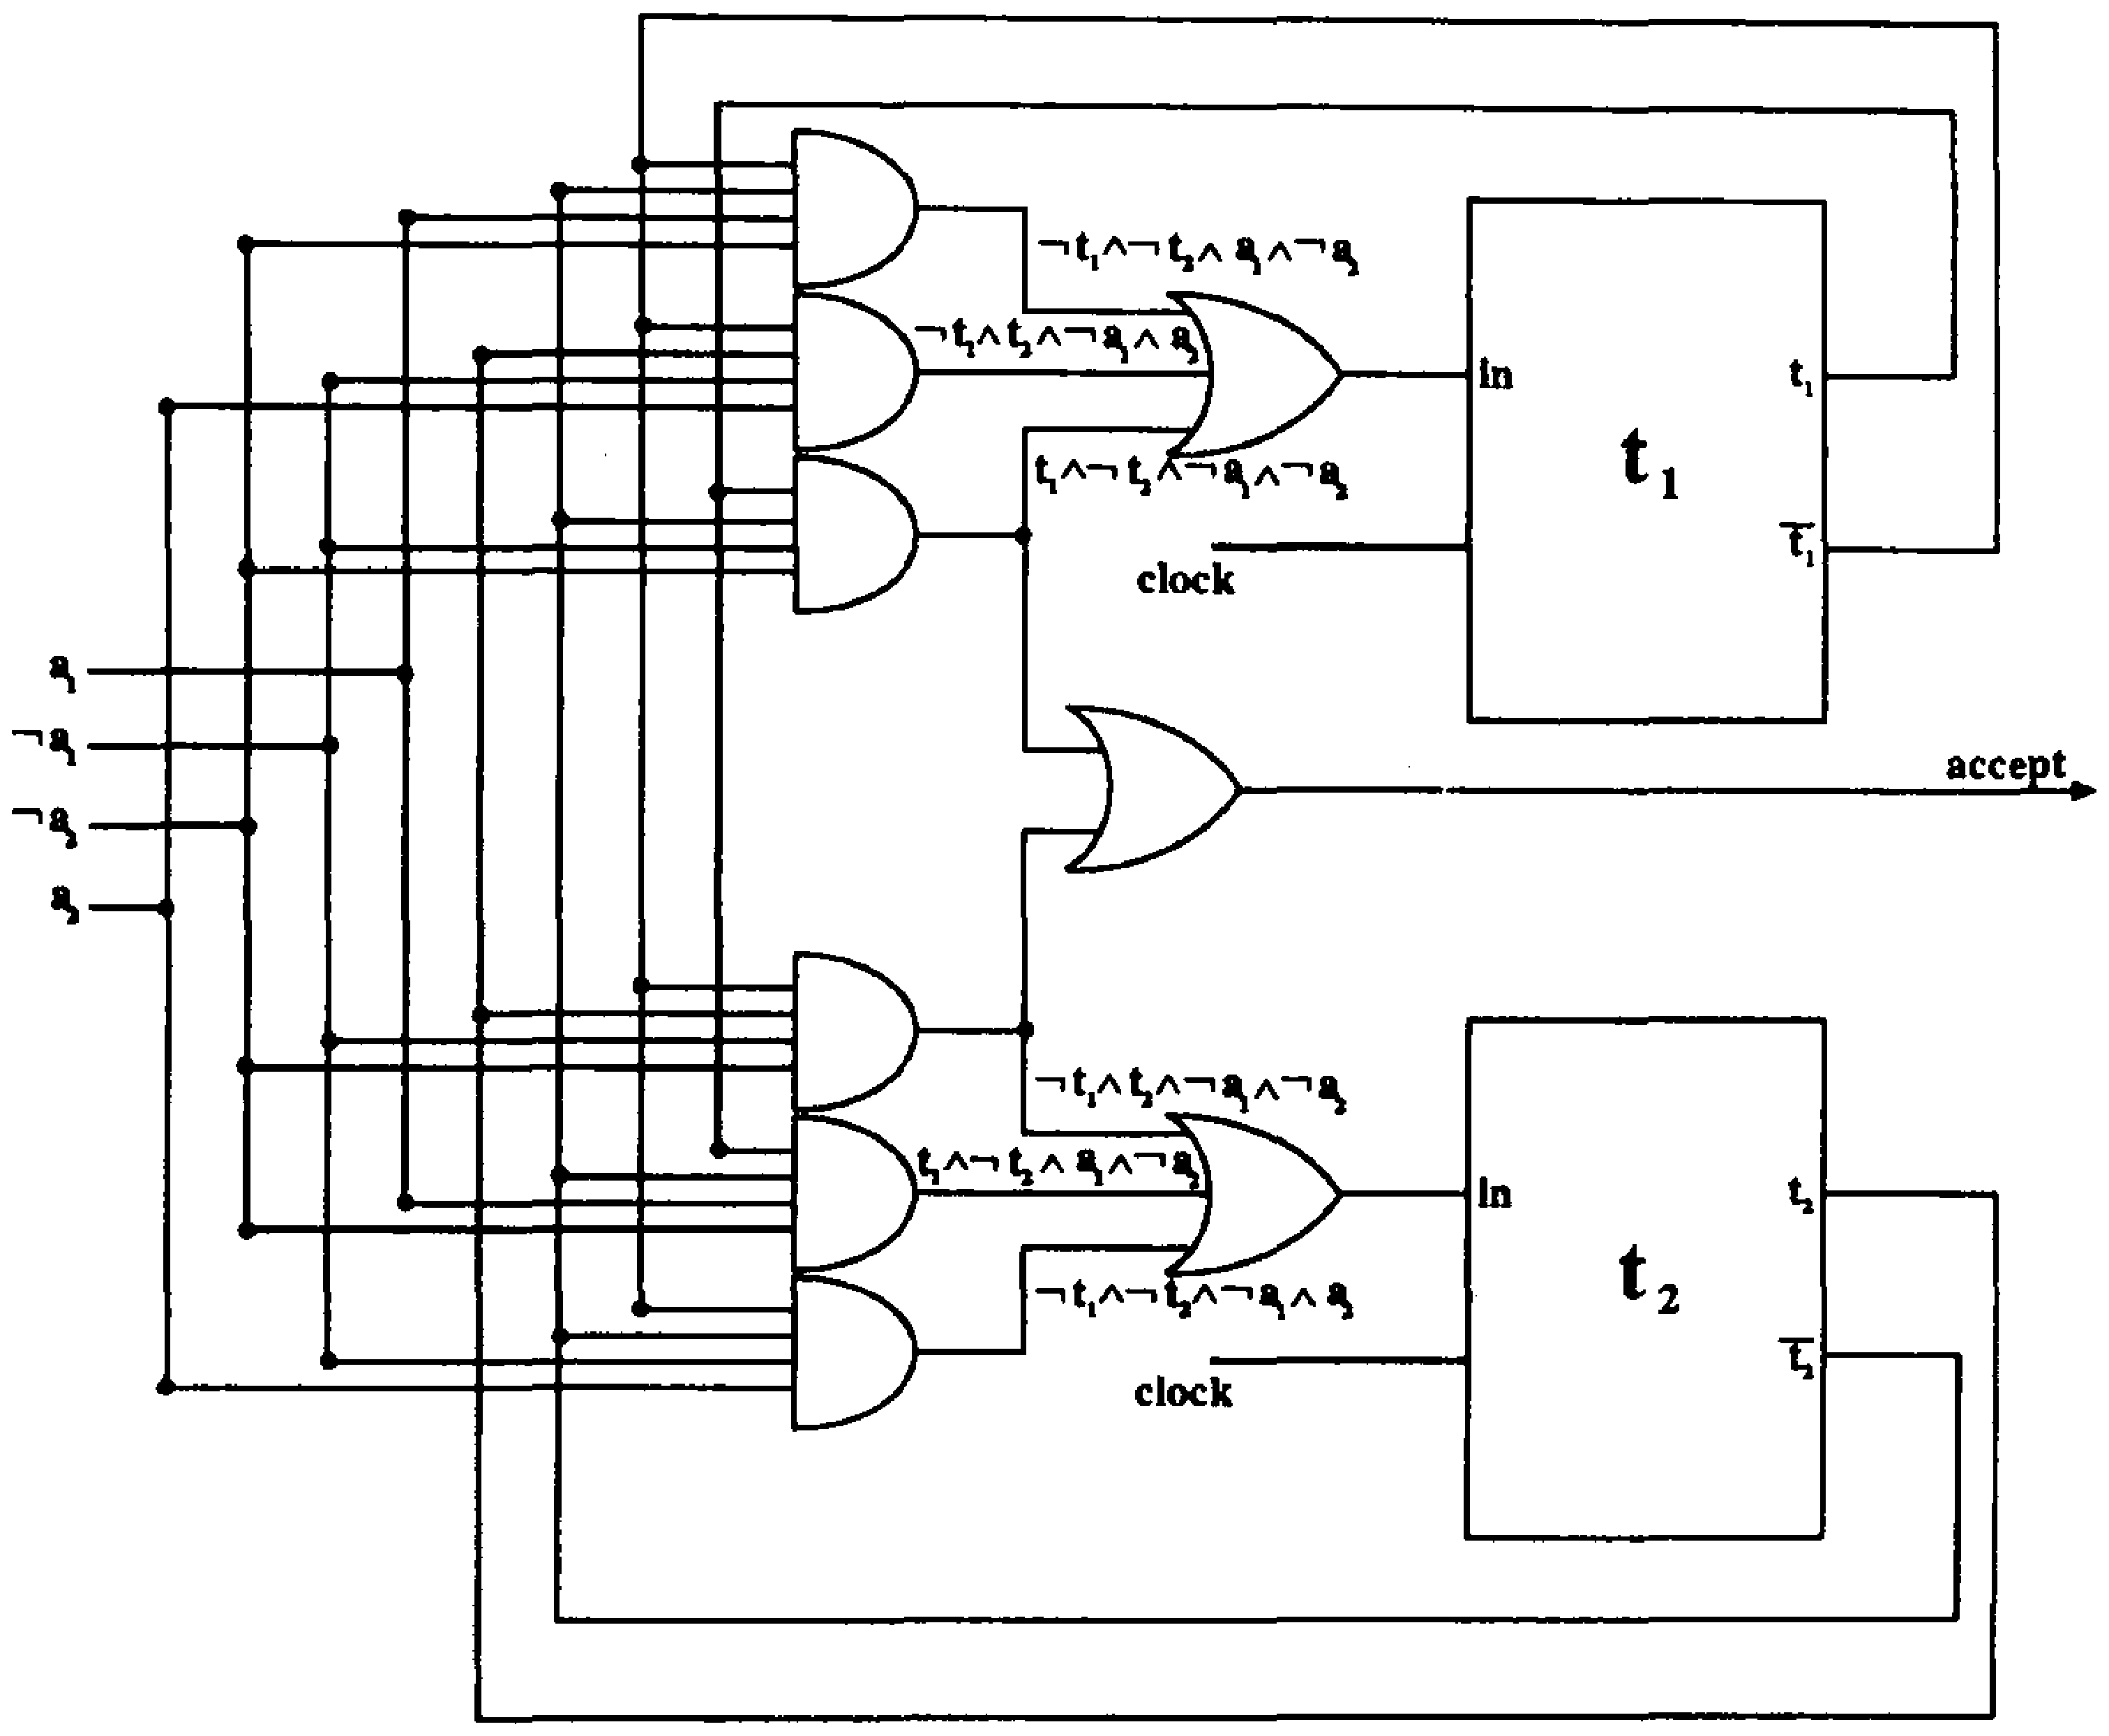
\epsfig{figure=ToFAfigures/fig1-21.eps,height=3.8in}}
\caption{The circuitry implementing the DFA discussed in Example 1.13}\label{fig-1.21}
\end{figure}

\section{Applications of Finite Automata}\label{sec-1.5}

In this chapter we have described the simplest form of finite automaton, the
DFA. Other forms of automata, such as nondeterministic finite automata, pushdown
automata, and Turing machines, are introduced later in the text. We close this 
chapter with three examples to motivate the material in the succeeding chapters.

When presenting automata in this chapter, we made no effort to construct the
\Index{minimal machine}.  A \emph{minimal} machine for a given language is one
that has the least number of states required to accept that language.

\subsection*{Example 1.14}

In Example 1.5, the vending machine kept track of the amount of change
that had been deposited up to $50$\cent. Since the candy bars cost only
30\cent, there is no need to count up to $50$\cent. In this sense, the machine
is not optimal, since a less complex machine can perform the same task, as shown
in Figure \ref{fig-1.22}. The corresponding quintuple is $\langle\{\pmb{n},
\pmb{d},\pmb{q}\},\{s_0,s_5,s_{10},s_{15},s_{20},s_{25},s_{30}\},s_0,\delta,
\{s_{30}\}\rangle$, where for each state $s_i$, $\delta$ is defined by
\begin{align*}
\delta(s_i,\pmb{n}) = s_{min\{30,i+5)\}} \\
\delta(s_i,\pmb{d}) = s_{min\{30,i+10\}} \\
\delta(s_i,\pmb{q}) = s_{min\{30,i+25\}}
\end{align*}

Note that the higher-numbered states in Example 1.5 were all
effectively ``remembering'' the same thing, that enough coins had been deposited.
These final states have been coalesced into a single final state to produce the
more efficient machine in Figure \ref{fig-1.22}. In the next two chapters, we
develop the theoretical background and algorithms necessary to construct from
an arbitrary DFA the minimal machine that accepts the same language.

As another illustration of the utility of concepts relating to finite-state
machines, we will consider the formalism used by many text editors to search for
a particular target string pattern in a text file. To find $\pmb{ababb}$ in a
file, for example, a naive approach might consist of checking whether the first
five characters of the file fit this pattern, and next checking characters 2
through 6 to find a match, and so on. This results in examining file characters
more than once; it ought to be possible to remember past values, and avoid such
duplication. Consider the text string $\pmb{aabababbb}$. By the time the fifth
character is scanned, we have matched the first four characters of $\pmb{ababb}$.
Unfortunately, $\pmb{a}$, the sixth character of $\pmb{aabababbb}$, does not produce
the final match; however, since characters 4,5, and 6 ($\pmb{aba}$) now match the
first three characters of the target string, it does allow for the possibility
of characters 4 through 8 matching (as is indeed the case in this example). This
leads to a general rule: If we have matched the first four letters of the target
string, and the next character happens to be $\pmb{a}$ (rather than the desired
$\pmb{b}$), we must remember that we have now matched the first three letters of
the target string.

% Figure 1.22
\begin{figure}
\centerline{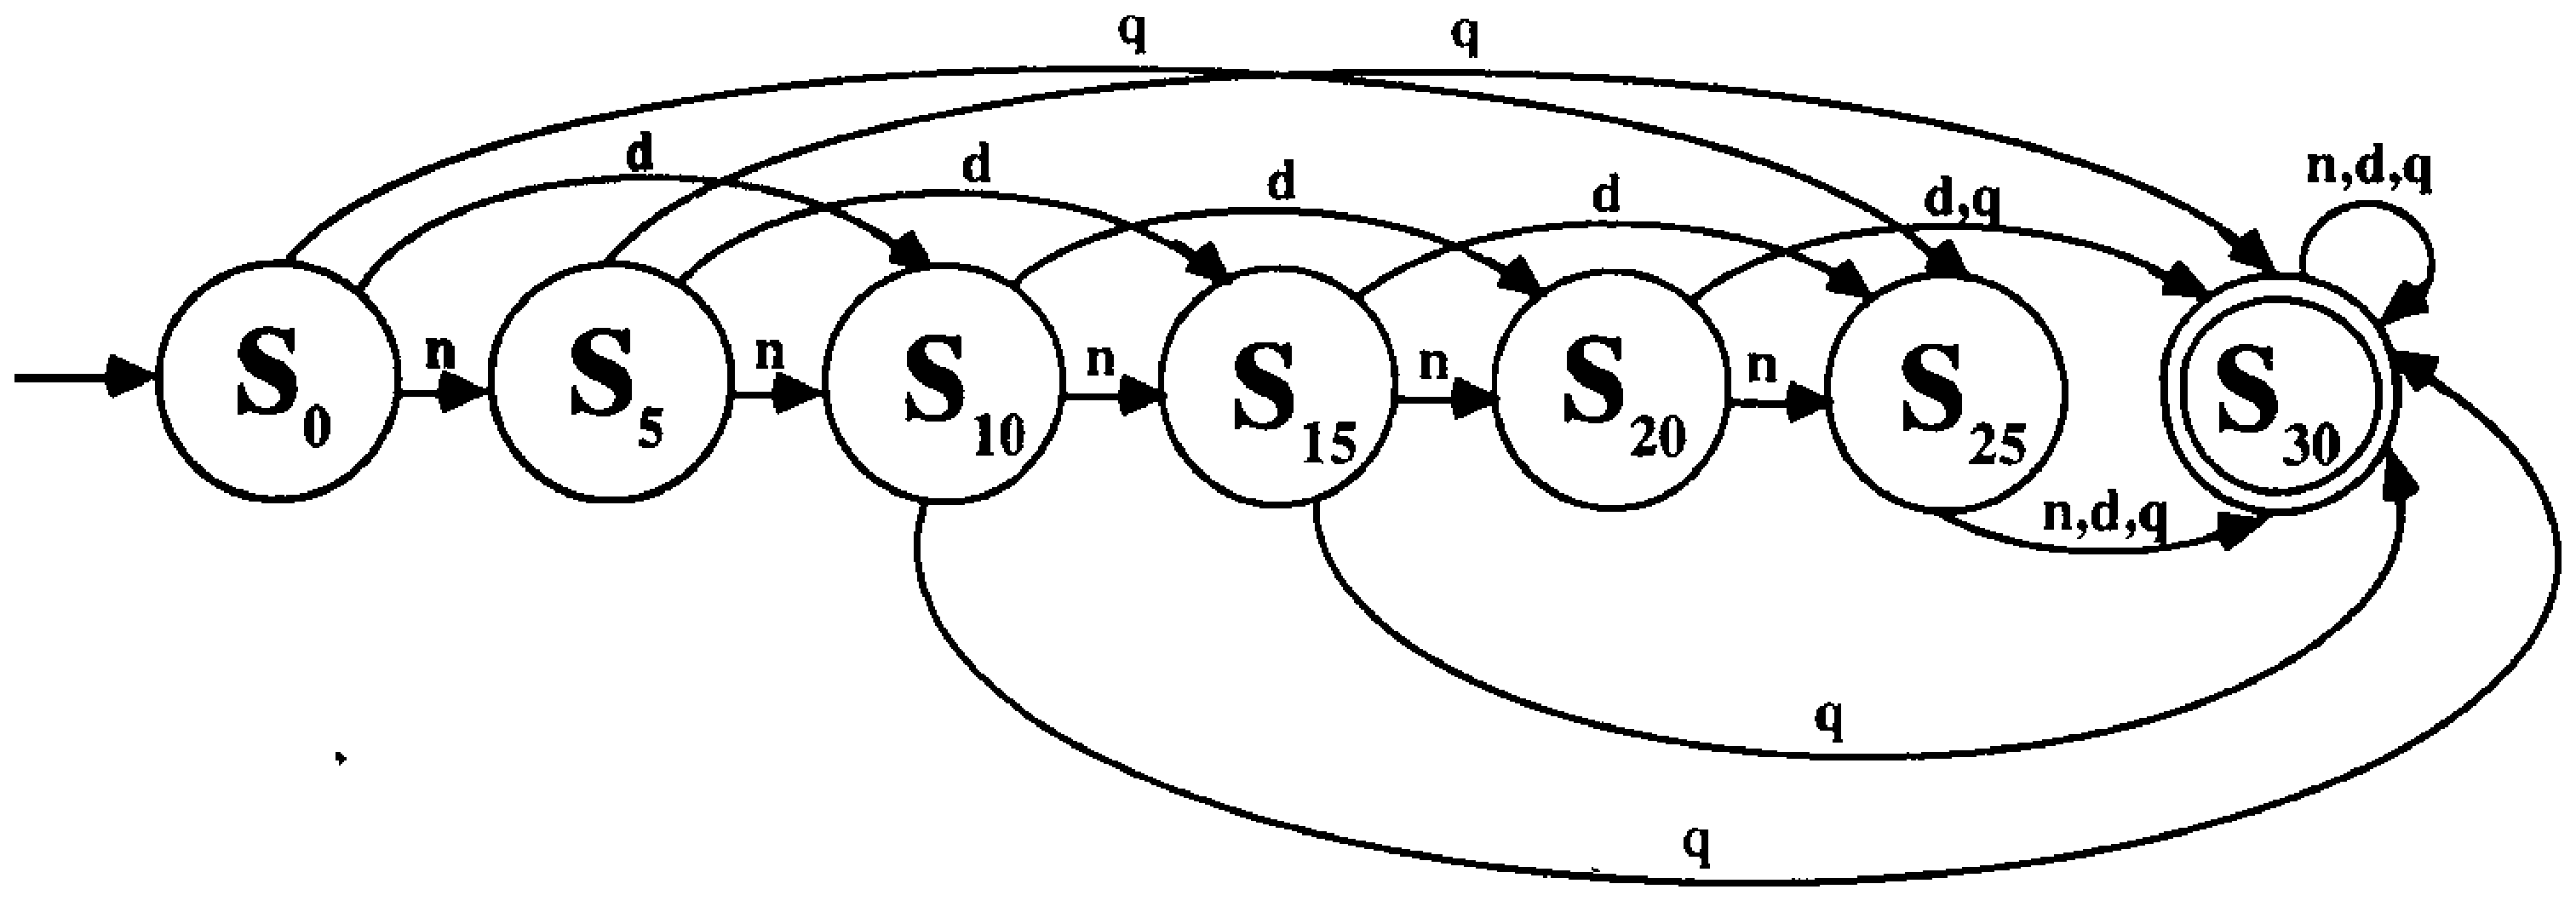
\epsfig{figure=ToFAfigures/fig1-22.eps,width=5.5in}}
\caption{The automaton discussed in Example 1.14}\label{fig-1.22}
\end{figure}

``Rules'' such as these are actually the state transitions in the DFA given in
the next example. State $s_i$ represents having matched the first $i$ characters
of the target string, and the rule developed above is succinctly stated as
$\delta(s_4,\pmb{a})=s_3$.

\subsection*{Example 1.15}

A DFA that accepts all strings that contain $\pmb{ababb}$ as a substring is
displayed in Figure \ref{fig-1.23}. The corresponding quintuple is
\[ \langle\{\pmb{a},\pmb{b}\},\{s_0,s_1,s_2,s_3,s_4,s_5\},s_0,\delta,\{s_5\}
	\rangle, \]
where $\delta$ is defined by
\begin{center}\begin{tabular}{c|cc}
$\delta$ & $\pmb{a}$ & $\pmb{b}$ \\
\hline
$s_0$ & $s_1$ & $s_0$ \\
$s_1$ & $s_1$ & $s_2$ \\
$s_2$ & $s_3$ & $s_0$ \\
$s_3$ & $s_1$ & $s_4$ \\
$s_4$ & $s_3$ & $s_5$ \\
$s_5$ & $s_5$ & $s_5$
\end{tabular}\end{center}

% Figure 1.23
\begin{figure}
\centerline{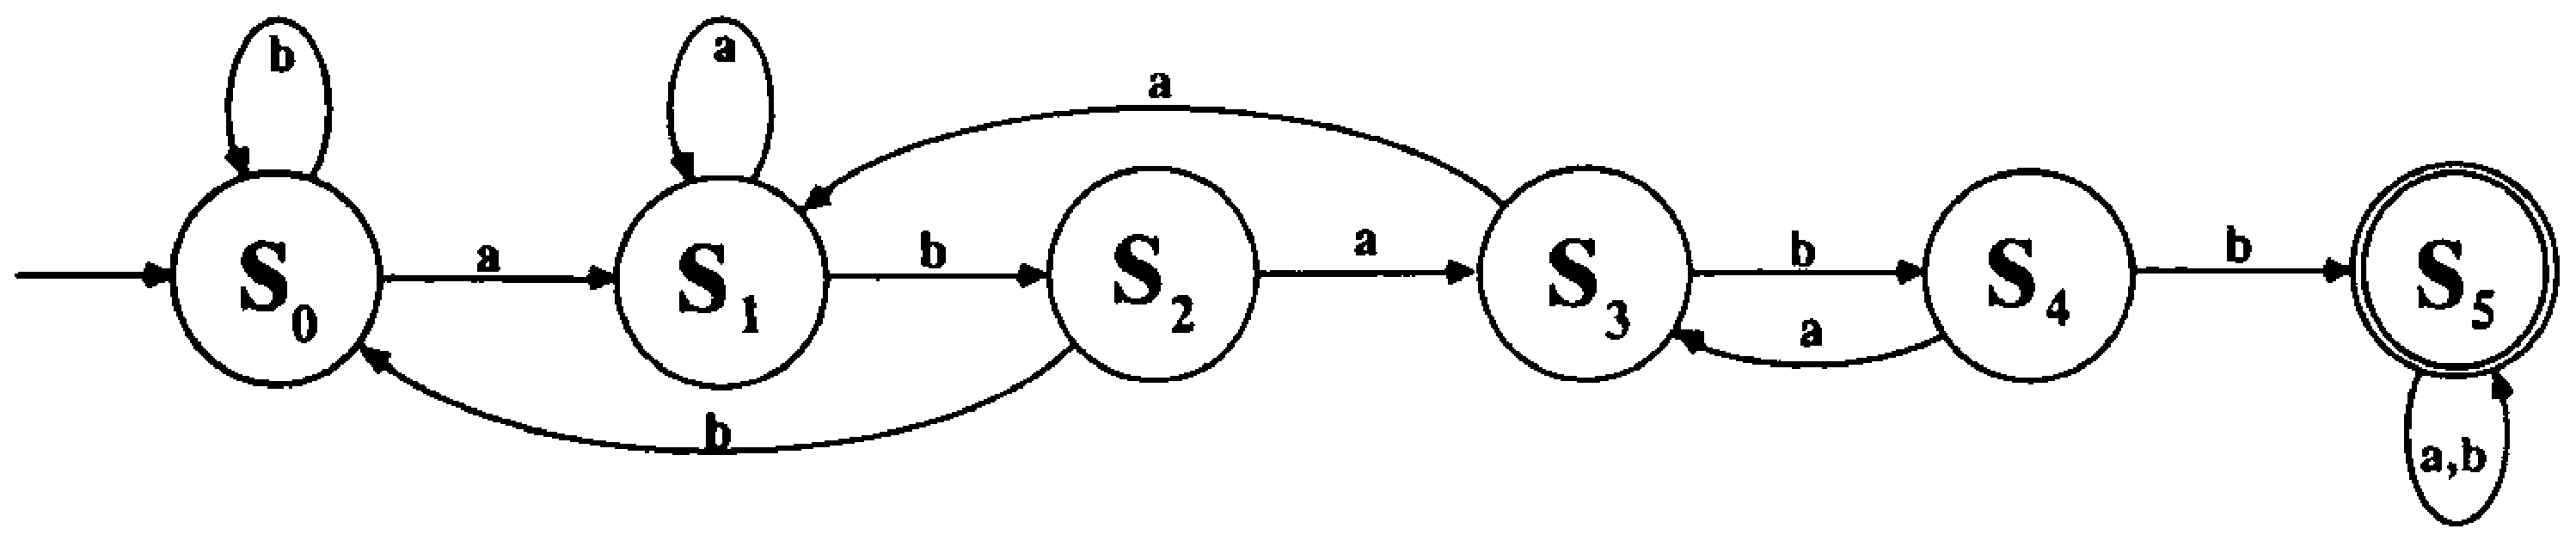
\epsfig{figure=ToFAfigures/fig1-23.eps,width=6.5in}}
\caption{A DFA that accepts strings containing $\pmb{ababb}$}\label{fig-1.23}
\end{figure}

It is a worthwhile exercise to test the operation of this DFA on several text
strings and verify that the automaton is indeed in state $s_i$ exactly when it
has matched the first $i$ characters of the target string. Note that if we did
not care what the third character of the substring was (that is, if we were
searching for occurrences of $\pmb{ababb}$ or $\pmb{abbbb}$), a trivial modification
of the above machine would allow us to search for both substrings at once, as
shown in Figure \ref{fig-1.24}. The corresponding quintuple is
$\langle\{\pmb{a},\pmb{b}\},\{s_0,s_1,s_2,s_3,s_4,s_5\},s_0,\delta,\{s_5\}\rangle$, where
$\delta$ is defined by
\begin{center}\begin{tabular}{c|cc}
$\delta$ & $\pmb{a}$ & $\pmb{b}$ \\
\hline
$s_0$ & $s_1$ & $s_0$ \\
$s_1$ & $s_1$ & $s_2$ \\
$s_2$ & $s_3$ & $s_3$ \\
$s_3$ & $s_1$ & $s_4$ \\
$s_4$ & $s_3$ & $s_5$ \\
$s_5$ & $s_5$ & $s_5$
\end{tabular}\end{center}

% Figure 1.24
\begin{figure}[h]
\centerline{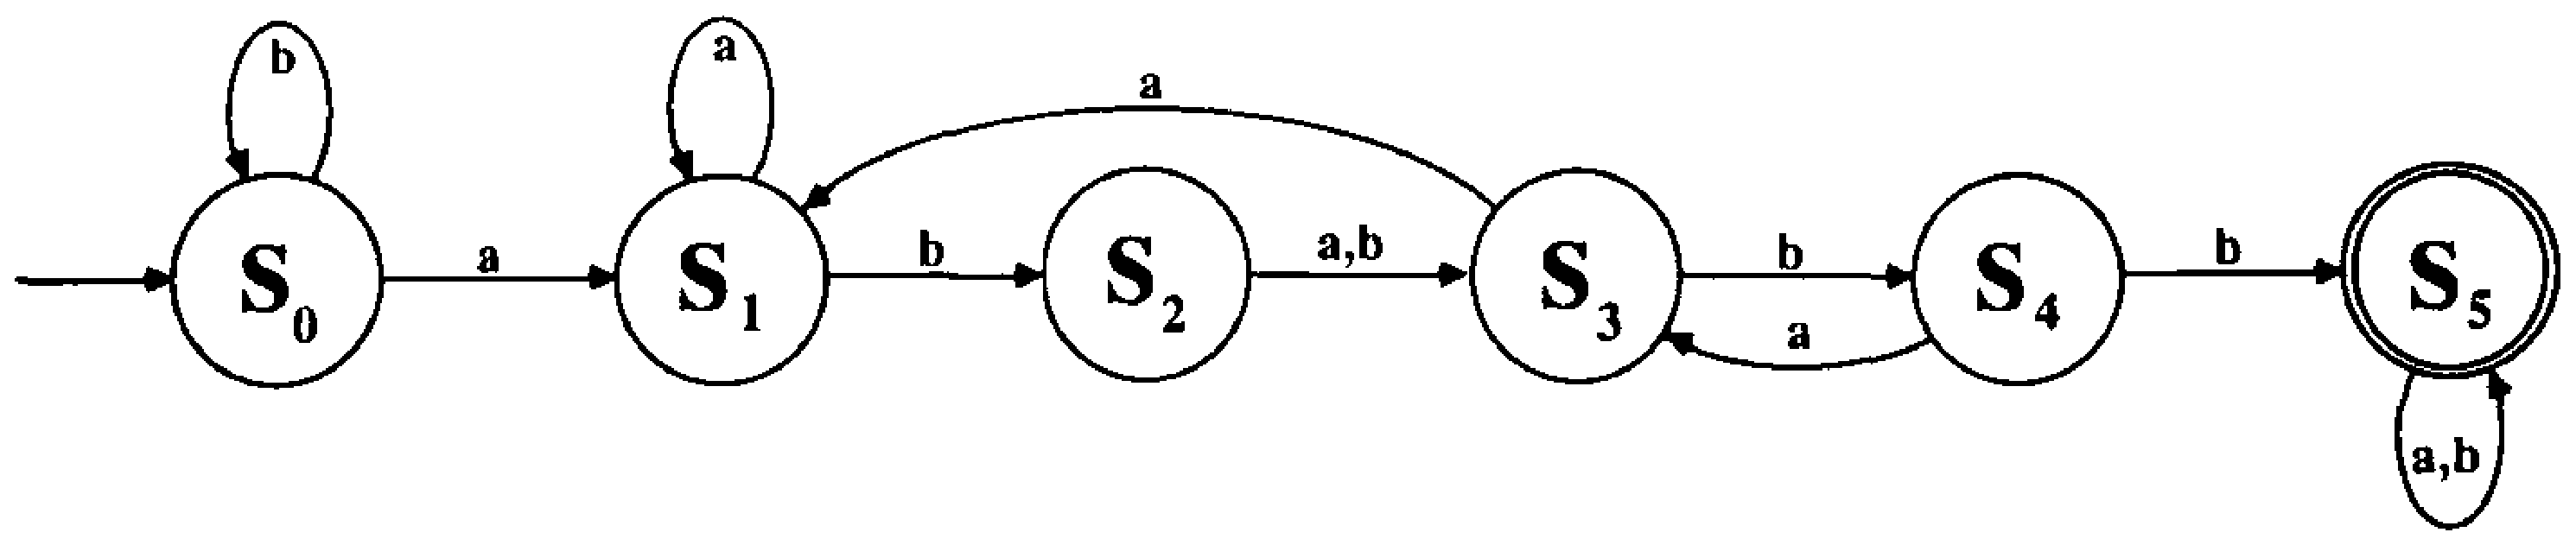
\epsfig{figure=ToFAfigures/fig1-24.eps,width=6.5in}}
\caption{A DFA that accepts strings that contain either $\pmb{ababb}$ or
$\pmb{abbbb}$}\label{fig-1.24}
\end{figure}
In this case, we required one letter between the initial part of the search
string ($\pmb{ab}$) and the terminal part ($\pmb{bb}$). It is possible to modify
the machine to accept strings that contain $\pmb{ab}$, followed by any number of
letters, followed by $\pmb{bb}$. This type of machine would be useful for
identifying \emph{comments} in many programming languages. For example, a Pascal
comment is essentially of the form $\pmb{(^*}$, followed by most combinations
of letters, followed by the first occurrence of $\pmb{^*)}$.

It should be noted that the machine in Example 1.15 is highly
specialized and tailored for the specific string $\pmb{ababb}$; other target
strings would require completely different recognizers. While it appears to
require much thought to generate the appropriate DFA for a given string, we will
see how the tools presented in Chapter \ref{ch-4} can be used to automate the
entire process.

Example 1.15 indicates how automata can be used to guide the construction of
software for matching designated patterns. Finite-state machines are also useful
in designing hardware that detects designated sequences. Example 4.7 will
explore a communications application, and the following discussion illustrates
how these concepts can be applied to help evaluate the performance of computers.

A computer program is essentially a linear list of machine instructions, stored
in consecutive memory locations. Each memory location holds a sequence of bits
that can be thought of as words comprised of $\pmb{0}$s and $\pmb{1}$s.
Different types of instructions are represented by different patterns of bits.
The CPU sequentially \emph{fetches} these instructions and chooses its next
action by examining the incoming bit pattern to determine the type of
instruction that should be executed. The sequences of bits that encode the
instruction type are called \emph{\Index{opcodes}}.

Various performance advantages can be attained when one part of the CPU
\emph{prefetches} the next instruction while another part executes the current
instruction. However, computers must have the capability of altering the order
in which instructions are executed; \emph{branch} instructions \index{branch instructions} allow the
CPU to avoid the anticipated next instruction and instead begin executing the
instructions stored in some other area of memory. When a branch occurs, the
prefetched instruction will generally need to be replaced by the proper
instruction from the new area of memory. The consequent delay can degrade the
speed with which instructions are executed.

Irrespective of prefetching problems, it should be clear that a branch
instruction followed immediately by another branch instruction is inefficient.
If a CPU is found to be regularly executing two or more consecutive branch
instructions, it may be worthwhile to consider replacing such series of branches
with a single branch to the ultimate destination [FERR]. Such information would
be determined by monitoring the instruction stream and searching for patterns
that represented consecutive branch opcodes. This activity is essentially the
pattern recognition problem discussed in Example 1.15.

It is unwise to try to collect the data representing the contents of the
instruction stream on secondary storage so that it can be analyzed later. The
volume of information and the speed with which it is generated preclude the
collection of a sufficiently large set of data points. Instead, the preferred
solution uses a specially tailored piece of hardware to monitor the contents of
the CPU opcode register and increment a hardware counter each time the
appropriate patterns are detected. The heart of this monitor can be built by
transforming the appropriate automaton into the corresponding logic circuitry,
as outlined in Section \ref{sec-1.4}. Unlike the automaton in Example 1.15,
the automaton model for this application would allow transitions out of the final
state, so that it may continue to search for successive patterns. The resulting
logic circuitry would accept as input the bit patterns currently present in the
opcode register, and send a pulse to the counter mechanism each time the accept
circuitry was energized.

Note that in this case we would not want to inhibit the accept circuitry by
requiring an \<EOS\> symbol to be scanned. Indeed, we want the light on our
conceptual black box to flicker as we process the data, since we are intent on
counting the number of times it flickers during the course of our monitoring.

\subsection*{Example 1.16}

We close this chapter with an illustration of the manner in which computational
algorithms can profitably use the automaton abstraction. Network communications
between independent processors are governed by a \emph{\Index{protocol}} that
implements a finite state control [TANE]. The \emph{Kermit} protocol,\index{Kermit protocol!DFA implementation}
developed at Columbia University, was widely employed to communicate between
processors and is still most often used for its original purpose: to transfer
files between micros and mainframes [DACR]. During a file transfer, the send
portion of Kermit on the source host is responsible for delivering data to the
receive portion of the Kermit process on the destination host. The receive
portion of Kermit reacts to incoming data in much the same way as the machines
presented in this chapter. The receive program \emph{starts} in a state of waiting for
a transfer request (in the form of an initialization packet) to signal the
commencement of a file transfer (state R in Figure \ref{fig-1.25}). When such
a packet is received, Kermit \emph{transitions} to the RF state, where it awaits a
file-header packet (which specifies the name of the file about to be transferred).
Upon receipt of the file-header packet, it enters the RD state, where it processes
a succession of data packets (which comprise the body of the file being
transferred). An \Index{EOF packet} should arrive after all the data are sent, which can
then be followed by another file-header packet (if there is a sequence of files
to be transferred) or by a break packet (if the transfer is complete). In the
latter case, Kermit reverts to the start state R and awaits the next transfer
request. The send portion of the Kermit process on the source host follows the
behavior of a slightly more complex automaton. The state transition diagram
given in Figure \ref{fig-1.25} succinctly describes the logic of the receive
portion of the Kermit protocol; for simplicity, timeouts and error conditions
are not reflected in the diagram. The input alphabet is \{B,D,Z,H,S\}, where B
represents a break, D is a data packet, Z is EOF, H is a file-header packet, and
S is a send-intention packet. The state set is \{A,R,RF,RD\}, where A denotes
the \underline{\emph{a}}bort state, R signifies \underline{\emph{r}}eceive,
RF is \underline{\emph{r}}eceive \underline{\emph{f}}ileheader, and RD is
\underline{\emph{r}}eceive \underline{\emph{d}}ata. Note that unexpected packets (such as a data packet received in
the start state R or a break packet received when data packets are expected in
state RD) cause a transition to the abort state A.

% Figure 1.25
\begin{figure}
\centerline{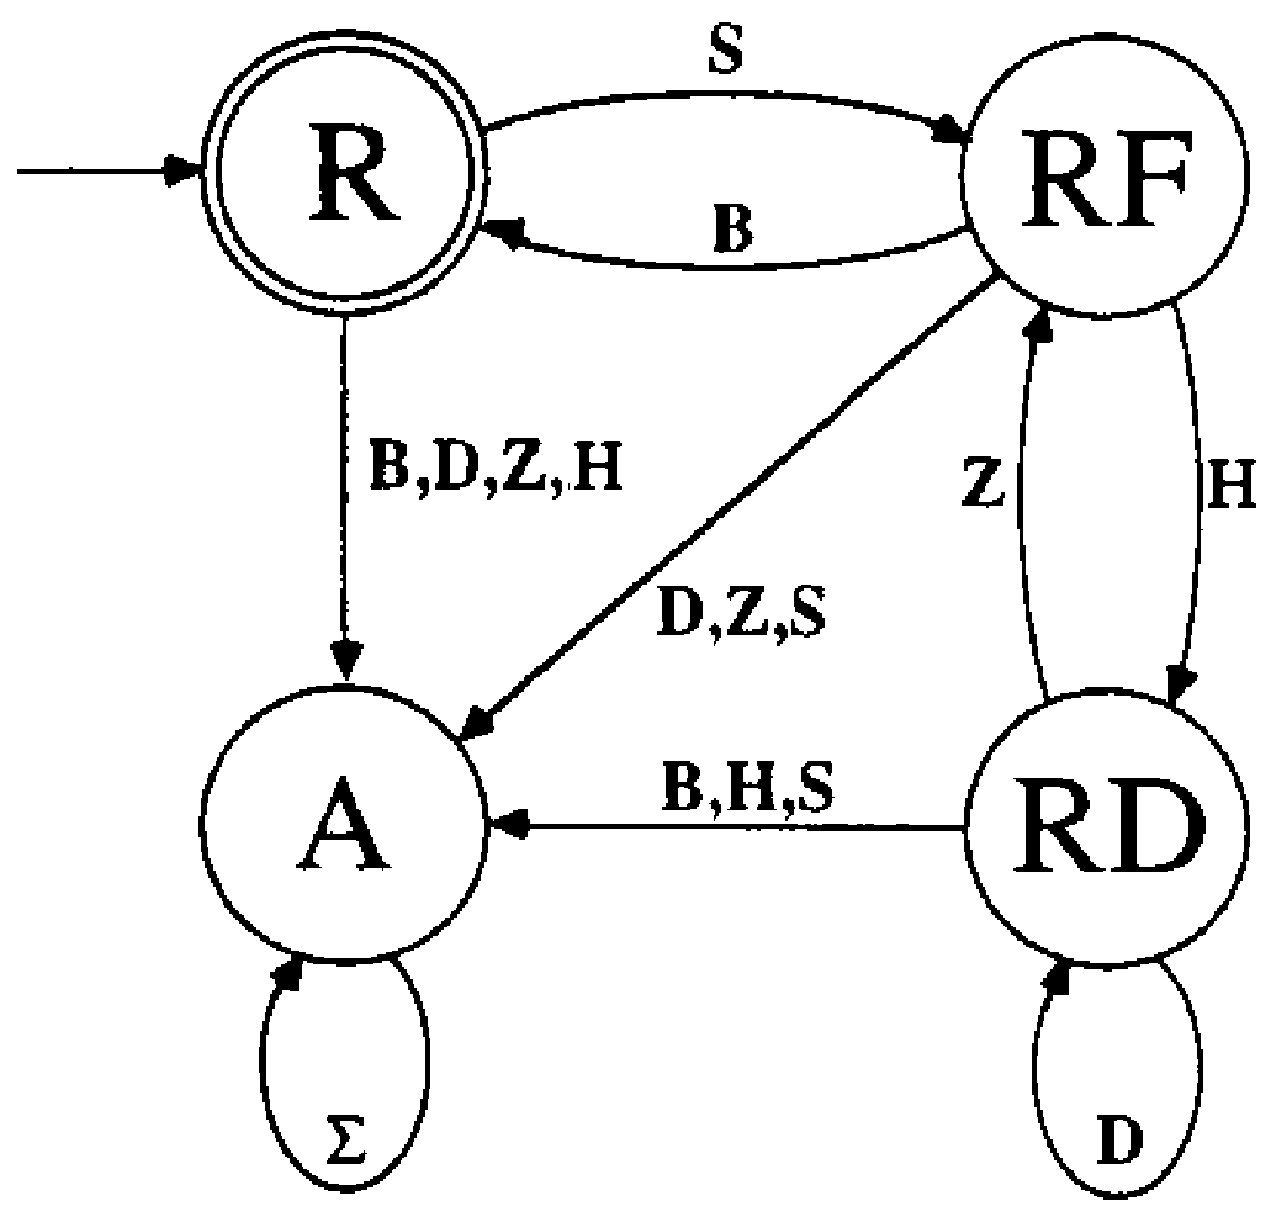
\epsfig{figure=ToFAfigures/fig1-25.eps,width=3.5in}}
\caption{The state transition diagram for the receive portion of Kermit, as
discussed in Example 1.16}\label{fig-1.25}
\end{figure}

In actuality, the receive protocol does more than just observe the incoming
packets; Kermit sends an acknowledgment (ACK or NAK)\index{ACK|see{Kermit protocol}}\index{NAK|see{Kermit protocol}} of each packet back to
the source host. Receipt of the file header should also cause an appropriate
file to be created and opened, and each succeeding data packet should be
verified and its contents placed sequentially in the new file. A machine model
that incorporates actions in response to input is the subject of Chapter \ref{ch-7},
where automata with output are explored.

\section*{EXERCISES}\label{sec-1.ex}

\begin{enumerate}[{1.}1.]
\item Recall how we defined $\DBAR$ in this chapter:
\begin{center}\begin{tabular}{l@{$\qquad$}l}
$(\forall s\in S)(\forall\pmb{a}\in \Sigma)$ & $\DBAR_t(s,\pmb{a})=\delta(s,
	\pmb{a})$ \\
$(\forall s\in S)$ & $\DBAR_t(s,\lambda)=s$ \\
$(\forall s\in S)(\forall x\in\Sigma^*)(\forall\pmb{a}\in\Sigma)$ & $\DBAR_t
	(s,\pmb{a}x)=\DBAR_t(\delta(s,\pmb{a}),x)$
\end{tabular}\end{center}
$\DBAR$, here denoted $\DBAR_t$, was tail recursive. Tail recursion means that
all recursion takes place at the end of the string. Let us now define an
alternative extended transition function, $\DBAR_h$, thusly:
\begin{center}\begin{tabular}{l@{$\qquad$}l}
$(\forall s\in S)(\forall\pmb{a}\in\Sigma)$ & $\DBAR_h(s,\pmb{a})=\delta(s,
	\pmb{a})$ \\
$(\forall s\in S)$ & $\DBAR_h(s,\lambda)=s$ \\
$(\forall s\in S)(\forall\pmb{a}\in\Sigma)(\forall x\in\Sigma^*)$ & $\DBAR_h
	(s,x\pmb{a})=\delta(\DBAR_h(s,x),\pmb{a})$
\end{tabular}\end{center}
It is clear from the definition of $\DBAR_h$ that all the recursion
takes place at the head of the string. For this reason, $\DBAR_h$ is
called \emph{\Index{head recursive}}. Show that the two definitions result in
the same extension of $\delta$, that is, prove by mathematical induction that
\[ (\forall s\in S)(\forall x\in\Sigma^*)(\DBAR_t(s,x)=\DBAR_h(s,x)) \]

\item Consider Example 1.14. The vending machine accepts coins as input, but if
you change your mind (or find you do not have enough change), it will not
refund your money. Modify this example to have another input, \<coin-return\>,
which is represented by $\pmb{r}$ and which will conceptually return all your
coins.

\item\label{exer1.3}
\begin{enumerate}
  \item Specify the quintuple corresponding to the DFA displayed in Figure \ref{fig-1.26}.
  \item Describe the language defined by the DFA displayed in Figure \ref{fig-1.26}.
\end{enumerate}

% Figure 1.26
\begin{figure}[h]
\centerline{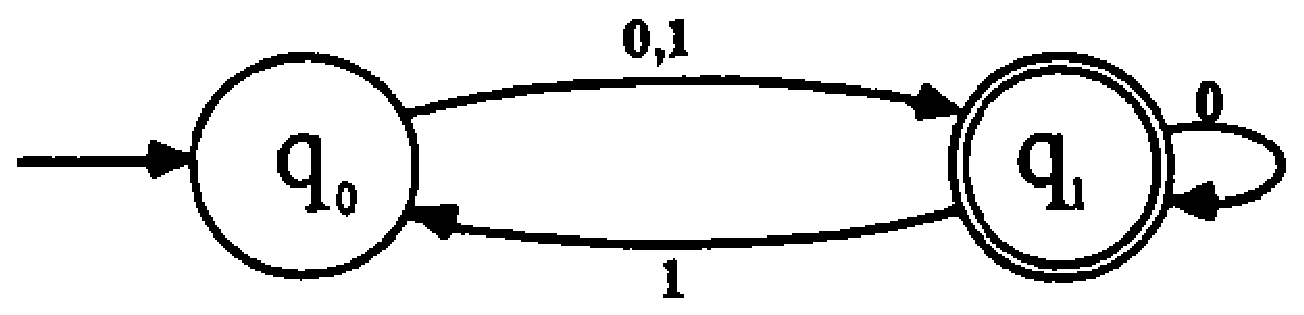
\epsfig{figure=ToFAfigures/fig1-26.eps,width=3.5in}}
\caption{The automaton discussed in Exercise 1.\ref{exer1.3}}\label{fig-1.26}
\end{figure}

\item Construct a state transition diagram and enumerate all five parts of a
deterministic finite automaton $A=\langle\{\pmb{a},\pmb{b},\pmb{c}\},S,s_0,
\delta,F\rangle$ such that
\[ L(A) = \{x \ | \ \ \ |x|\text{ is a multiple of }2\text{ or }3\}. \]

\item Let $\Sigma = \{\pmb{0},\pmb{1}\}$. Construct deterministic finite
automata that will accept each of the following languages, if possible.
\begin{enumerate}
\item $L_1=\{x \ |\ \ \ |x| \bmod 7 = 4\}$
\item $L_2=\Sigma^*-\{w\ | \ \exists n\geq 1\ni w=\pmb{a}_1\ldots \pmb{a}_n\wedge \pmb{a}_n = 1\}$
\item $L_3=\{y \ | \ \ \ |y|_0=|y|_1\}$
\end{enumerate}

\item Let $\Sigma = \{\pmb{a},\pmb{b}\}$.
\begin{enumerate}
\item Construct deterministic finite automata $A_1$, $A_2$, $A_3$, and $A_4$
such that:
\begin{enumerate}
\item $L(A_1)=\{x\ |\ (|x|_a\text{ is odd})\wedge(|x|_b\text{ is even})\}$
\item $L(A_2)=\{y\ |\ (|y|_a\text{ is even})\vee(|y|_b\text{ is odd})\}$
\item $L(A_3)=\{z\ |\ (|z|_a\text{ is even})\overline{\vee}(|z|_b\text{ is even})\}
	\ \ (\overline{\vee}\text{ represents exclusive-or})$
\item $L(A_4)=\{z\ | \ \ \ |z|_a\text{ is even}\}$
\end{enumerate}
\item How does the structure of each of these machines relate to the one defined
in Example 1.10?
\end{enumerate}

\item Modify the machine $M$ defined in Example 1.10 so that the language
accepted by the machine consists of strings $x\in\{\pmb{a},\pmb{b}\}^*$, where
both $|x|_{\pmb{a}}$ and $|x|_{\pmb{b}}$ are even and $|x|>0$, that is, the new
machine should accept $L(M) - \{\lambda\}$.

\item Let $M=\langle\Sigma,S,s_0,\delta,F\rangle$ be an (arbitrary) DFA that accepts the
language $L(M)$. Write down a general procedure for modifying this machine so
that it will accept $L(M) - \{\lambda\}$. (Specify the five parts of the new
machine and justify your statements.) It may be helpful to do this for a
specific machine (as in Exercise 1.7) before attempting the general case.

\item Let $M=\langle\Sigma,S,s_0,\delta,F\rangle$ be an (arbitrary) DFA that accepts the
language $L(M)$. Write down a general procedure for modifying this machine so
that it will accept $L(M)\cup\{\lambda\}$. (Specify the five parts of the new
machine and justify your statements.)

\item Let $\Sigma=\{\pmb{a},\pmb{b},\pmb{d}\}$ and $\Psi=\{x\in\Sigma^*
 \ | \ (x\text{ begins with }\pmb{d})\vee(x\text{ contains two consecutive $\pmb{b}$s})\}$.
\begin{enumerate}
\item Draw a machine that will accept $\Psi$.
\item Formally specify the five parts of the DFA from part (a).
\end{enumerate}

\item Let $\Sigma=\{\pmb{a},\pmb{b},\pmb{c}\}$ and $\Phi=\{x \in \Sigma^*
	|\text{ every $\pmb{b}$ in $x$ is immediately followed by }\pmb{c}\}$.
\begin{enumerate}
\item Draw a machine that will accept $\Phi$.
\item Formally specify the five parts of the DFA from part (a).
\end{enumerate}

\item Let $\Sigma=\{\pmb{0},\pmb{1},\pmb{2},\pmb{3},\pmb{4},\pmb{5},\pmb{6},
\pmb{7},\pmb{8},\pmb{9}\}$. Consider the base 10 numbers formed by strings from
$\Sigma^*$: $\pmb{14}$ represents fourteen, the three-digit string $\pmb{205}$
represents two hundred and five, and so on. Let $\Omega=\{x \in \Sigma^*
|$ the number represented by $x$ is evenly divisible by $7$\} = 
$\{\lambda,\pmb{0},\pmb{00},\pmb{000},\ldots,\pmb{7},\pmb{07},\pmb{007},\ldots,
\pmb{14},\pmb{21},\pmb{28},\pmb{35},\ldots\}$.
\begin{enumerate}
\item Draw a machine that will accept $\Omega$.
\item Formally specify the five parts of the DFA from part (a).
\end{enumerate}

\item Let $\Sigma=\{\pmb{0},\pmb{1},\pmb{2},\pmb{3},\pmb{4},\pmb{5},\pmb{6},
\pmb{7},\pmb{8},\pmb{9}\}$. Let $\Gamma=\{x\in \Sigma^*|$ the number represented
by $x$ is evenly divisible by $3$\}.
\begin{enumerate}
\item Draw a three-state machine that will accept $\Gamma$.
\item Formally specify the five parts of the DFA from part (a).
\end{enumerate}

\item Let $\Sigma=\{\pmb{0},\pmb{1},\pmb{2},\pmb{3},\pmb{4},\pmb{5},\pmb{6},
\pmb{7},\pmb{8},\pmb{9}\}$. Let $K=\{x\in \Sigma^*|$ the number represented by
$x$ is evenly divisible by $5$\}.
\begin{enumerate}
\item Draw a five-state DFA that accepts $K$.
\item Formally specify the five parts of the DFA from part (a).
\item Draw a two-state DFA that accepts $K$.
\item Formally specify the five parts of the DFA from part (c).
\end{enumerate}

\item Let $\Sigma=\{\pmb{0},\pmb{1},\pmb{2},\pmb{3},\pmb{4},\pmb{5},\pmb{6},
\pmb{7},\pmb{8},\pmb{9}\}$. Draw a DFA that accepts the first eight primes.

\item \begin{enumerate}
\item Find all ten combinations of $u$, $v$, and $w$ such
that $uvw=\pmb{cab}$ (one such combination is $u=\pmb{c}$, $v=\lambda$,
$w=\pmb{ab}$).
\item In general, if $x$ is of length $n$, and $uvw = x$, how many distinct
combinations of $u$, $v$, and $w$ will satisfy this constraint?
\end{enumerate}

\item Let $\Sigma = \{\pmb{a},\pmb{b}\}$ and $\Xi =\{x \in \Sigma^*|x$ contains
(at least) two consecutive $\pmb{b}$s $\wedge\ x$ does \emph{not} contain two
consecutive $\pmb{a}$s\}. Draw a machine that will accept $\Xi$.

\item The FORTRAN identifier in Example 1.9 recognized \emph{all} alphabetic
words, including those like DO, DATA, END, and STOP, which have different uses
in FORTRAN. Modify Figure \ref{fig-1.11} to produce a DFA that will also reject
the words DO and DATA while still accepting all other valid FORTRAN identifiers.

\item Consider the machine defined in Example 1.11. This machine
accepts most real number constants in scientific notation. However, this machine
does have some (possibly desirable) limitations. These limitations include
requiring that a $\pmb{0}$ precede the decimal point when specifying a number
with a mantissa less than 1.
\begin{enumerate}
\item Modify Figure \ref{fig-1.13} so that it will accept the set of real-number
constants described by the following BNF.
\begin{center}
%\begin{tabular}{r@{ ::}l}
\begin{tabular}{rllll}
\<sign\> & $::=$ & $ \pmb{+}|\pmb{-}$ & \\
\<digit\> &  $::=$ & $ \pmb{0}|\pmb{1}|\pmb{2}|\pmb{3}|\pmb{4}|\pmb{5}|\pmb{6}|\pmb{7}|
	\pmb{8}|\pmb{9}$ & \\
\<natural\> & $::=$ & \<digit\>$|$\<digit\>\<natural\> & \\
\<integer\> & $::=$ & \<natural\>$|$\<sign\>\<natural\> & \\
\<real constant\> & $::=$& \<integer\> & $|$ \\
&& \<integer\>{\bf .} & $|$ \\
&& {\bf .}\<natural\> & $|$ \\
&& \<sign\>{\bf .}\<natural\> & $|$ \\
&& {\bf .}\<natural\>{\bf E}\<integer\> & $|$ \\
&& \<sign\>{\bf .}\<natural\>{\bf E}\<integer\> & $|$ \\
&& \<integer\>{\bf .}\<natural\> & $|$ \\
&& \<integer\>{\bf .}\<natural\>{\bf E}\<integer> & \\
\end{tabular}
\end{center}
\item Write a program in your favorite programming language to implement the
automaton derived in part (a). The program should read a line of text and state
whether or not the word on that line was accepted.
\end{enumerate}

\item Show that part (i) of Definition \ref{dfn-1.11} is implied by parts (ii)
and (iii) of that definition.

\item Develop a more succinct description of the transition function given in
Example 1.9 (compare with the description in Example 1.10).

\item Let the universal set be $\{\pmb{a,b}\}^*$. Give an example of
\begin{enumerate}
\item A finite set.
\item A cofinite\index{cofinite!set} set.
\item A set that is neither finite nor cofinite.
\end{enumerate}

\item\label{q-states} Consider the DFA given in Figure \ref{fig-1.27}.
\begin{enumerate}
\item Specify the quintuple for this machine.
\item Describe the language defined by this machine.
\end{enumerate}

% Figure 1.27
\begin{figure}
\centerline{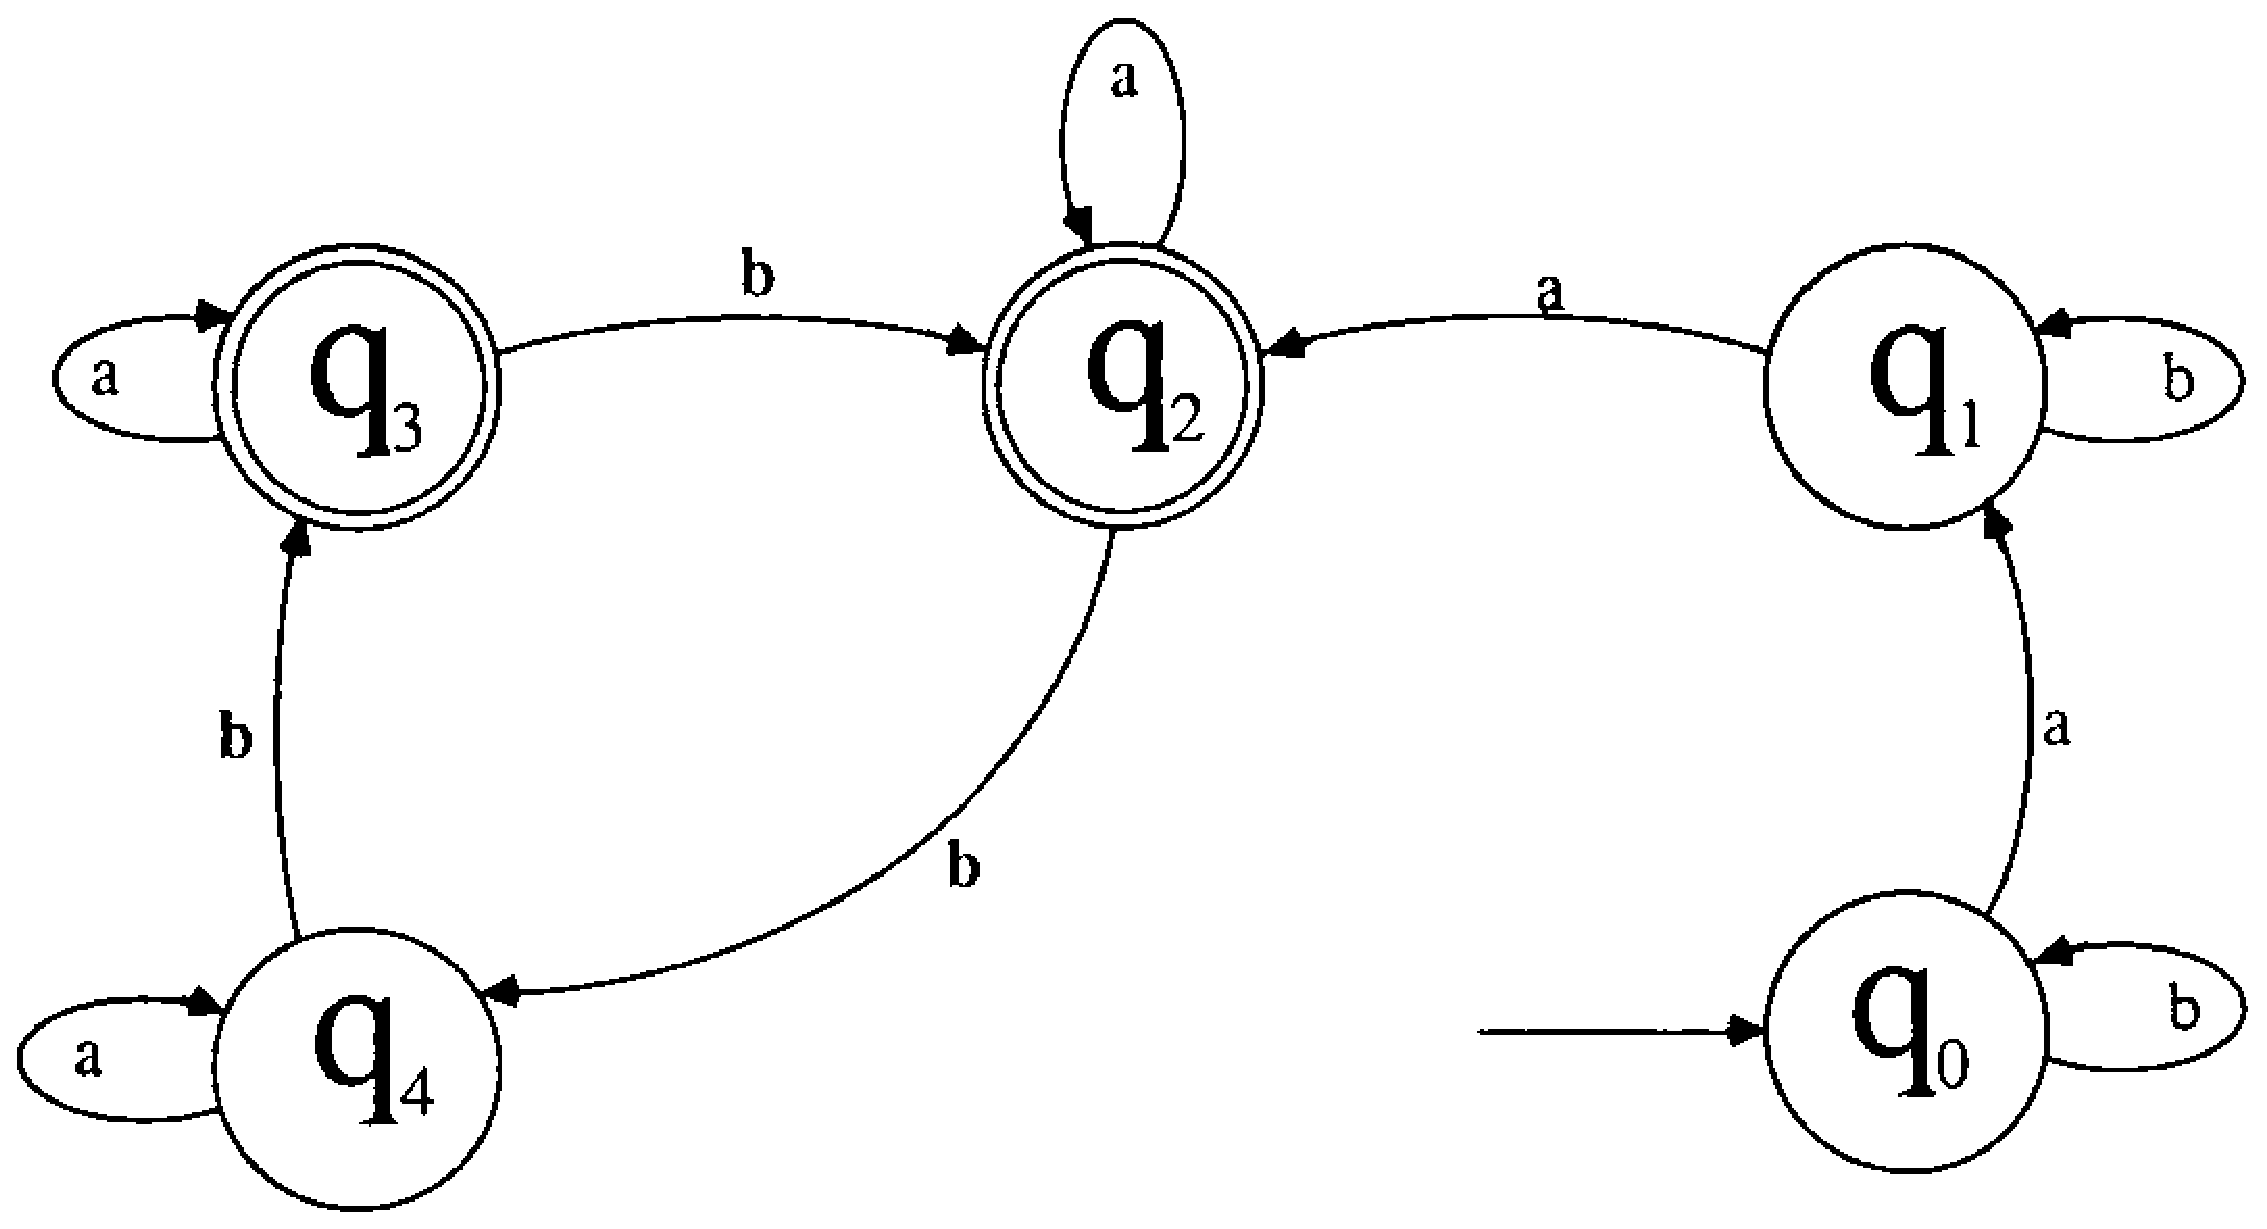
\epsfig{figure=ToFAfigures/fig1-27.eps,width=5in}}
\caption{The DFA discussed in Exercise 1.\ref{q-states}}\label{fig-1.27}
\end{figure}

\item Consider the set consisting of the names of everyone in China. Is this set
a FAD language?

\item Consider the set of all legal infix arithmetic expressions over the
alphabet $\{\pmb{A},\pmb{B},\pmb{+},\pmb{-},\pmb{\times},\pmb{/}\}$ without
parentheses (assume normal precedence rules apply). Is this set a FAD language?
If so, draw the machine.
(Assume that $\pmb{-}$ represents both negation and subtraction.)

\item Consider an arbitrary deterministic finite automaton $M$.
\begin{enumerate}
\item What aspect of the machine determines whether $\lambda \in L(M)$?
\item Specify a condition that would guarantee that $L(M) = \Sigma^*$.
\item Specify a condition that would guarantee that $L(M) = \emptyset$.
\end{enumerate}

\item Construct deterministic finite automata to accept each of the following
languages.
\begin{enumerate}
\item $\{x\in\{\pmb{a},\pmb{b},\pmb{c}\}^* |\  \ \pmb{abc}\text{ is a substring of }x\}$
\item $\{x\in\{\pmb{a},\pmb{b},\pmb{c}\}^* |\  \ \pmb{acaba}\text{ is a substring of }x\}$
\end{enumerate}

\item Consider Example 1.14. The vending machine had as input nickels,
dimes, and quarters. When 30\cent\  had been deposited, a candy bar could be
selected. Modify this machine to also accept pennies, denoted by $p$, as an
additional input. How does this affect the number of states in the machine?

\item\label{t-states} \begin{enumerate}
\item Describe the language defined by the following quintuple (compare with
Figure \ref{fig-1.28}).
\begin{center}\begin{tabular}{l@{$\qquad$}l}
$\Sigma=\{\pmb{a},\pmb{b}\}$ & $\delta(t_0,\pmb{a})=t_0$ \\
$S=\{t_0,t_1\}$ & $\delta(t_0,\pmb{b})=t_1$ \\
$s_0=t_0$ & $\delta(t_1,\pmb{a})=t_1$ \\
$F=\{t_1\}$ & $\delta(t_1,\pmb{b})=t_0$
\end{tabular}\end{center}
\item Rigorously \emph{prove} the statement you made in part (a). \emph{Hint:} First
prove the inductive statement
\[ P(n):(\forall x \in \Sigma^n)((\DBAR(t_0,x)=t_0\Leftrightarrow|x|_{\pmb{b}}
\text{ is even}) \wedge (\DBAR(t_0,x)=t_1\Leftrightarrow|x|_{\pmb{b}}
\text{ is odd})). \]
\end{enumerate}

% Figure 1.28
\begin{figure}
\centerline{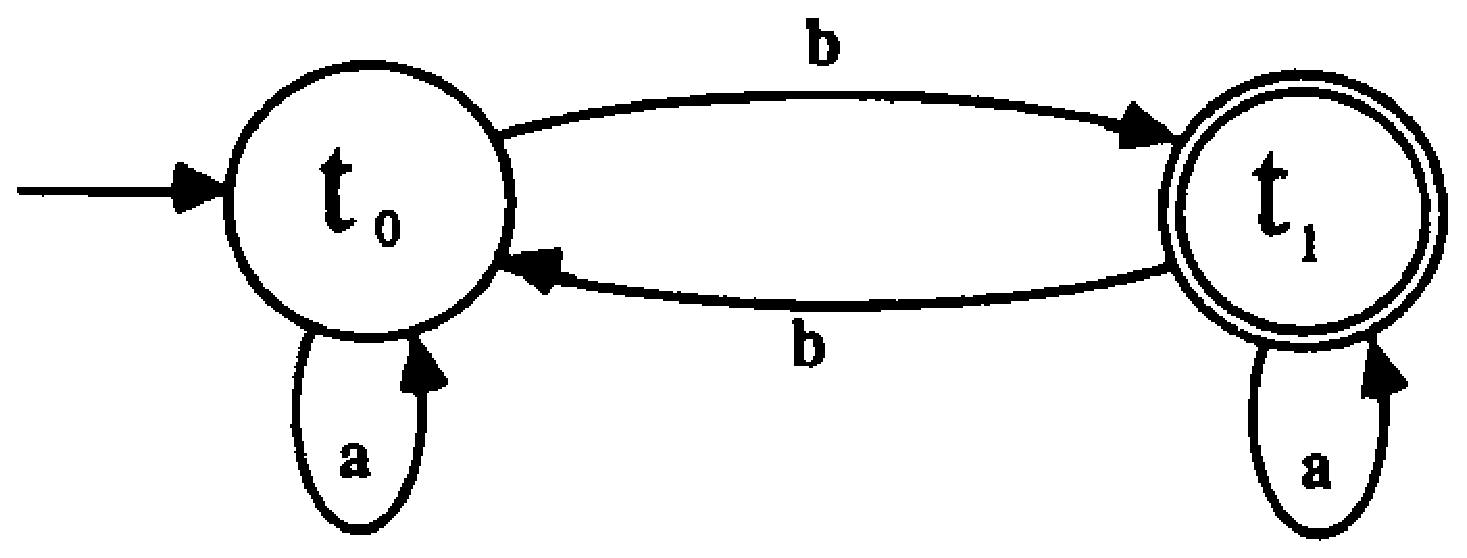
\epsfig{figure=ToFAfigures/fig1-28.eps,width=3in}}
\caption{The DFA discussed in Exercise 1.\ref{t-states}}\label{fig-1.28}
\end{figure}

\item Consider a vending machine that accepts as input pennies, nickels, dimes,
and quarters and dispenses 10\cent\  candy bars.
\begin{enumerate}
\item Draw a DFA that models this machine.
\item Define the quintuple for this machine.
\item How many states are absolutely necessary to build this machine?
\end{enumerate}

\item Consider a vending machine that accepts as input nickels, dimes, and
quarters and dispenses 10\cent\  candy bars.
\begin{enumerate}
\item Draw a DFA that models this machine.
\item How many states are absolutely necessary to build this machine?
\item Using the standard encoding conventions, draw a circuit diagram for this
machine (include \<EOS\> but not \<SOS\> in the input alphabet).
\end{enumerate}

\item Using the standard encoding conventions, draw a circuit diagram that will
implement the machine given in Exercise 1.29, as follows:
\begin{enumerate}
\item Implements both \<EOS\> and \<SOS\>.
\item Uses neither \<EOS\> nor \<SOS\>.
\end{enumerate}

\item Using the standard encoding conventions, draw a circuit diagram that will
implement the machine given in Exercise 1.7, as follows:
\begin{enumerate}
\item Implements both \<EOS\> and \<SOS\>.
\item Uses neither \<EOS\> nor \<SOS\>.
\end{enumerate}

\item Modify Example 1.12 so that it correctly handles the \<SOS\> symbol; draw
the new circuit diagram.

\item Using the standard encoding conventions, draw a circuit diagram that will
implement the machine given in Example 1.6, as follows:
\begin{enumerate}
\item Implements both \<EOS\> and \<SOS\>.
\item Uses neither \<EOS\> nor \<SOS\>.
\end{enumerate}

\item Using the standard encoding conventions, draw a circuit diagram that will
implement the machine given in Example 1.10, as follows:
\begin{enumerate}
\item Implements both \<EOS\> and \<SOS\>.
\item Uses neither \<EOS\> nor \<SOS\>.
\end{enumerate}

\item Using the standard encoding conventions, draw a circuit diagram that will
implement the machine given in Example 1.14 (include \<EOS\> but not \<SOS\> in
the input alphabet).

\item Using the standard encoding conventions, draw a circuit diagram that will
implement the machine given in Example 1.16; include the \<SOS\> and \<EOS\>
symbols.

\item Let $\Sigma=\{\pmb{a},\pmb{b},\pmb{c}\}$. Let $L=\{x\in\{\pmb{a},\pmb{b},
\pmb{c}\}^* \ | \ \ |x|_{\pmb{b}} = 2\}$.
\begin{enumerate}
\item Draw a DFA that accepts $L$.
\item Formally specify the five parts of a DFA that accepts $L$.
\end{enumerate}

\item Draw a DFA accepting $\{x\in\{\pmb{a},\pmb{b},\pmb{c}\}^*|$ every $\pmb{b}$
in $x$ is eventually followed by $\pmb{c}\}$; that is, $x$ might look like
$\pmb{baabacaa}$, or $\pmb{bcacc}$, and so on.

\item Let $\Sigma =\{\pmb{a},\pmb{b}\}$. Consider the language consisting of all
words that have neither consecutive $\pmb{a}$s nor consecutive $\pmb{b}$s.
\begin{enumerate}
\item Draw a DFA that accepts this language.
\item Formally specify the five parts of a DFA that accepts $L$.
\end{enumerate}

\item Let $\Sigma=\{\pmb{a},\pmb{b},\pmb{c}\}$. Let
$L=\{x\in\{\pmb{a},\pmb{b},\pmb{c}\}^* \,| \ \ |x|_{\pmb{a}} \equiv 0 \bmod 3\}$.
\begin{enumerate}
\item Draw a DFA that accepts $L$.
\item Formally specify the five parts of a DFA that accepts $L$.
\end{enumerate}

\item Let $\Sigma=\{\pmb{a},\pmb{b},\pmb{(},\pmb{*},\pmb{)}\}$. Recall that a
Pascal comment is essentially of the form: $\pmb{(*}$ followed by most
combinations of letters followed by the first occurrence of $\pmb{*)}$. While
the appropriate alphabet for Pascal is the ASCII\index{ASCII alphabet} character set, for simplicity
we will let $\Sigma=\{\pmb{a},\pmb{b},\pmb{(},\pmb{*},\pmb{)}\}$. Note that
$\pmb{(*b(*b(a)b*)}$ is a single valid comment, since all characters prior to
the first $\pmb{*)}$ (including the second $\pmb{(*}$ ) are considered part of
the comment. Consequently, comments cannot be nested.
\begin{enumerate}
\item Draw a DFA that recognizes all strings that contain exactly one valid
Pascal comment (and no illegal portions of comments, as in $\pmb{aa(*b*)b(*a)}$, which should be rejected).
\item Draw a DFA that recognizes all strings that contain zero or more valid
(that is, unnested) Pascal comments. For example,
$\pmb{a(*b(*bb*)ba*)aa}$ and $\pmb{a(*b}$ are not valid, while
$\pmb{a()a(**)b(*ab*)}$ is valid.
\end{enumerate}

\item
\begin{enumerate}
\item Is the set of all postfix expressions over $\{\pmb{A},\pmb{B},\pmb{+},
\pmb{-},\pmb{\times},\pmb{/}\}$ with two or fewer operators a FAD language? If it
is, draw a machine.
\item Is the set of all postfix expressions over $\{\pmb{A},\pmb{B},\pmb{+},
\pmb{-},\pmb{\times},\pmb{/}\}$ with four or fewer operators a FAD language? If it
is, draw a machine.
\item Is the set of all postfix expressions over $\{\pmb{A},\pmb{B},\pmb{+},
\pmb{-},\pmb{\times},\pmb{/}\}$ with eight or fewer operators a FAD language? If it
is, draw a machine.
\item Do you think the set of \emph{all} postfix expressions over $\{\pmb{A},\pmb{B},
\pmb{+},\pmb{-},\pmb{\times},\pmb{/}\}$ is a FAD language? Why or why not?
\end{enumerate}

\item Let $\Sigma =\{\pmb{a},\pmb{b},\pmb{c}\}$. Consider the language
consisting of all words that begin and end with different letters.
\begin{enumerate}
\item Draw a DFA that accepts this language.
\item Formally specify the five parts of a DFA that accepts this language.
\end{enumerate}

\item Let $\Sigma =\{\pmb{a},\pmb{b},\pmb{c}\}$.
\begin{enumerate}
\item Draw a DFA that rejects all words for which the last two letters match.
\item Formally specify the five parts of the DFA.
\end{enumerate}

\item Let $\Sigma =\{\pmb{a},\pmb{b},\pmb{c}\}$.
\begin{enumerate}
\item Draw a DFA that rejects all words for which the first two letters match.
\item Formally specify the five parts of the DFA.
\end{enumerate}

\item Prove that the empty word is unique; that is, using the definition of
equality of strings, show that if $x$ and $y$ are empty words then $x = y$.

\item For any two strings $x$ and $y$, show that $|xy| = |x| + |y|$

\item \begin{enumerate}
\item Draw the DFA corresponding to
$C=\langle\{\pmb{a},\pmb{b},\pmb{c}\},\{t_0,t_1\},t_0,\delta,\{t_1\}\rangle$,
where
\begin{center}\begin{tabular}{l@{$\qquad$}l}
$\delta(t_0,\pmb{a})=t_0$ & $\delta(t_1,\pmb{a})=t_0$ \\
$\delta(t_0,\pmb{b})=t_1$ & $\delta(t_1,\pmb{b})=t_1$ \\
$\delta(t_0,\pmb{c})=t_1$ & $\delta(t_1,\pmb{c})=t_0$
\end{tabular}\end{center}
\item Describe $L(C)$.
\item Using the standard encoding conventions, draw a circuit diagram for this
machine (include \<EOS\> but not \<SOS\> in the input alphabet).
\end{enumerate}

\item Let $\Sigma=\{\pmb{I},\pmb{V},\pmb{X},\pmb{L},\pmb{C},\pmb{D},\pmb{M}\}$.
Recall that $\pmb{VVI}$ is not considered to be a Roman numeral.
\begin{enumerate}
\item Draw a DFA that recognizes strict-order Roman numerals; that is, 9 must be
represented by $\pmb{VIIII}$ rather than $\pmb{IX}$, and so on.
\item Draw a DFA that recognizes the set of all Roman numerals; that is, 9 can
be represented by $\pmb{IX}$, 40 by $\pmb{XL}$, and so on.
\item Write a Pascal program based on your answer to part (b) that recognizes
the set of all Roman numerals.
\end{enumerate}

\item Describe the set of words accepted by the DFA in Figure \ref{fig-1.9}.

\item Let $\Sigma=\{\pmb{0},\pmb{1},\pmb{2},\pmb{3},\pmb{4},\pmb{5},\pmb{6},
\pmb{7},\pmb{8},\pmb{9}\}$. Let \\
$L_n=\{x \in \Sigma^* \ | \ $ the sum of the digits of $x$ is evenly divisible by
$n$\}. Thus, \\
$L_7=\{\lambda,\pmb{0},\pmb{7},\pmb{00},\pmb{07},\pmb{16},\pmb{25},\pmb{34},
\pmb{43},\pmb{52},\pmb{59},\pmb{61},\pmb{68},\pmb{70},\pmb{77},\pmb{86},\pmb{95},
\pmb{000},\pmb{007},\ldots\}$.
\begin{enumerate}
\item Draw a machine that will accept $L_7$.
\item Formally specify the five parts of the DFA given in part (a).
\item Draw a machine that will accept $L_3$.
\item Formally specify the five parts of the DFA given in part (c).
\item Formally specify the five parts of a DFA that will recognize $L_n$.
\end{enumerate}

\item Consider the last row of Table \ref{tbl-1.3}. Unlike the preceding three
rows, the outputs in this row are not marked with the don't-care symbol. Explain.

\end{enumerate}
